%%%%%%%%%%%%%%%%%%%%%%%%%%%%%%%%%%%%%%%%
% Beamer Presentation
% LaTeX Template
% Version 1.0 (10/11/12)
%
% This template has been downloaded from:
% http://www.LaTeXTemplates.com
%
% License:
% CC BY-NC-SA 3.0 (http://creativecommons.org/licenses/by-nc-sa/3.0/)
%
%%%%%%%%%%%%%%%%%%%%%%%%%%%%%%%%%%%%%%%%%

%----------------------------------------------------------------------------------------
%	PACKAGES AND THEMES
%----------------------------------------------------------------------------------------

\documentclass{beamer}

\mode<presentation> {

% The Beamer class comes with a number of default slide themes
% which change the colors and layouts of slides. Below this is a list
% of all the themes, uncomment each in turn to see what they look like.

%\usetheme{default}
%\usetheme{AnnArbor}
%\usetheme{Antibes}
%\usetheme{Bergen}
%\usetheme{Berkeley}
%\usetheme{Berlin}
%\usetheme{Boadilla}
%\usetheme{CambridgeUS}
%\usetheme{Copenhagen}
%\usetheme{Darmstadt}
%\usetheme{Dresden}
%\usetheme{Frankfurt}
%\usetheme{Goettingen}
%\usetheme{Hannover}
%\usetheme{Ilmenau}
%\usetheme{JuanLesPins}
%\usetheme{Luebeck}
\usetheme{Madrid}
%\usetheme{Malmoe}
%\usetheme{Marburg}
%\usetheme{Montpellier}
%\usetheme{PaloAlto}
%\usetheme{Pittsburgh}
%\usetheme{Rochester}
%\usetheme{Singapore}
%\usetheme{Szeged}
%\usetheme{Warsaw}

% As well as themes, the Beamer class has a number of color themes
% for any slide theme. Uncomment each of these in turn to see how it
% changes the colors of your current slide theme.

%\usecolortheme{albatross}
%\usecolortheme{beaver}
%\usecolortheme{beetle}
%\usecolortheme{crane}
%\usecolortheme{dolphin}
%\usecolortheme{dove}
%\usecolortheme{fly}
\usecolortheme{lily}
%\usecolortheme{orchid}
%\usecolortheme{rose}
%\usecolortheme{seagull}
%\usecolortheme{seahorse}
%\usecolortheme{whale}
%\usecolortheme{wolverine}

%\setbeamertemplate{footline} % To remove the footer line in all slides uncomment this line
%\setbeamertemplate{footline}[page number] % To replace the footer line in all slides with a simple slide count uncomment this line

%\setbeamertemplate{navigation symbols}{} % To remove the navigation symbols from the bottom of all slides uncomment this line
}
\definecolor{UBCblue}{rgb}{0.04706, 0.13725, 0.26667} % UBC Blue (primary)
\usecolortheme[named=UBCblue]{structure}
%\useoutertheme{miniframes} % Alternatively: miniframes, infolines, split
\useinnertheme{rectangles}

\usepackage{tikzsymbols}
\usepackage{graphicx} % Allows including images
\usepackage{booktabs} % Allows the use of \toprule, \midrule and \bottomrule in tables
\usepackage[style=authoryear, backend=bibtex]{biblatex}
\renewcommand*{\citesetup}{%
    \tiny
    \biburlsetup
    \frenchspacing}
\renewcommand*{\nameyeardelim}{\addcomma\addspace}
\addbibresource{bibio.bib}
%pdflatex myfile
%bibtex myfile
%pdflatex myfile
\usepackage{caption}
\captionsetup[figure]{font=tiny,labelfont=tiny, labelformat= empty}
\usepackage{stackengine}
%----------------------------------------------------------------------------------------
%	TITLE PAGE
%----------------------------------------------------------------------------------------

\title[CFD\&DL]{Solving Engineering Problems: Deep Learning (DL) for Computational Fluid Dynamics (CFD)} % The short title appears at the bottom of every slide, the full title is only on the title page

\author{S. Magda, A. Magda} % Your name
\institute[] % Your institution as it will appear on the bottom of every slide, may be shorthand to save space
{
n.g.\\ % Your institution for the title page
\medskip
\textit{} % Your email address
}
\date{\today} % Date, can be changed to a custom date

\begin{document}

\begin{frame}
\titlepage % Print the title page as the first slide
\end{frame}

\begin{frame}
\frametitle{Overview} % Table of contents slide, comment this block out to remove it
\tableofcontents % Throughout your presentation, if you choose to use \section{} and \subsection{} commands, these will automatically be printed on this slide as an overview of your presentation
\end{frame}

%----------------------------------------------------------------------------------------
%	PRESENTATION SLIDES
%----------------------------------------------------------------------------------------

%------------------------------------------------
\section{History} % Sections can be created in order to organize your presentation into discrete blocks, all sections and subsections are automatically printed in the table of contents as an overview of the talk

\begin{frame}
\frametitle{}%{It all started with ...}
\begin{figure}[h]
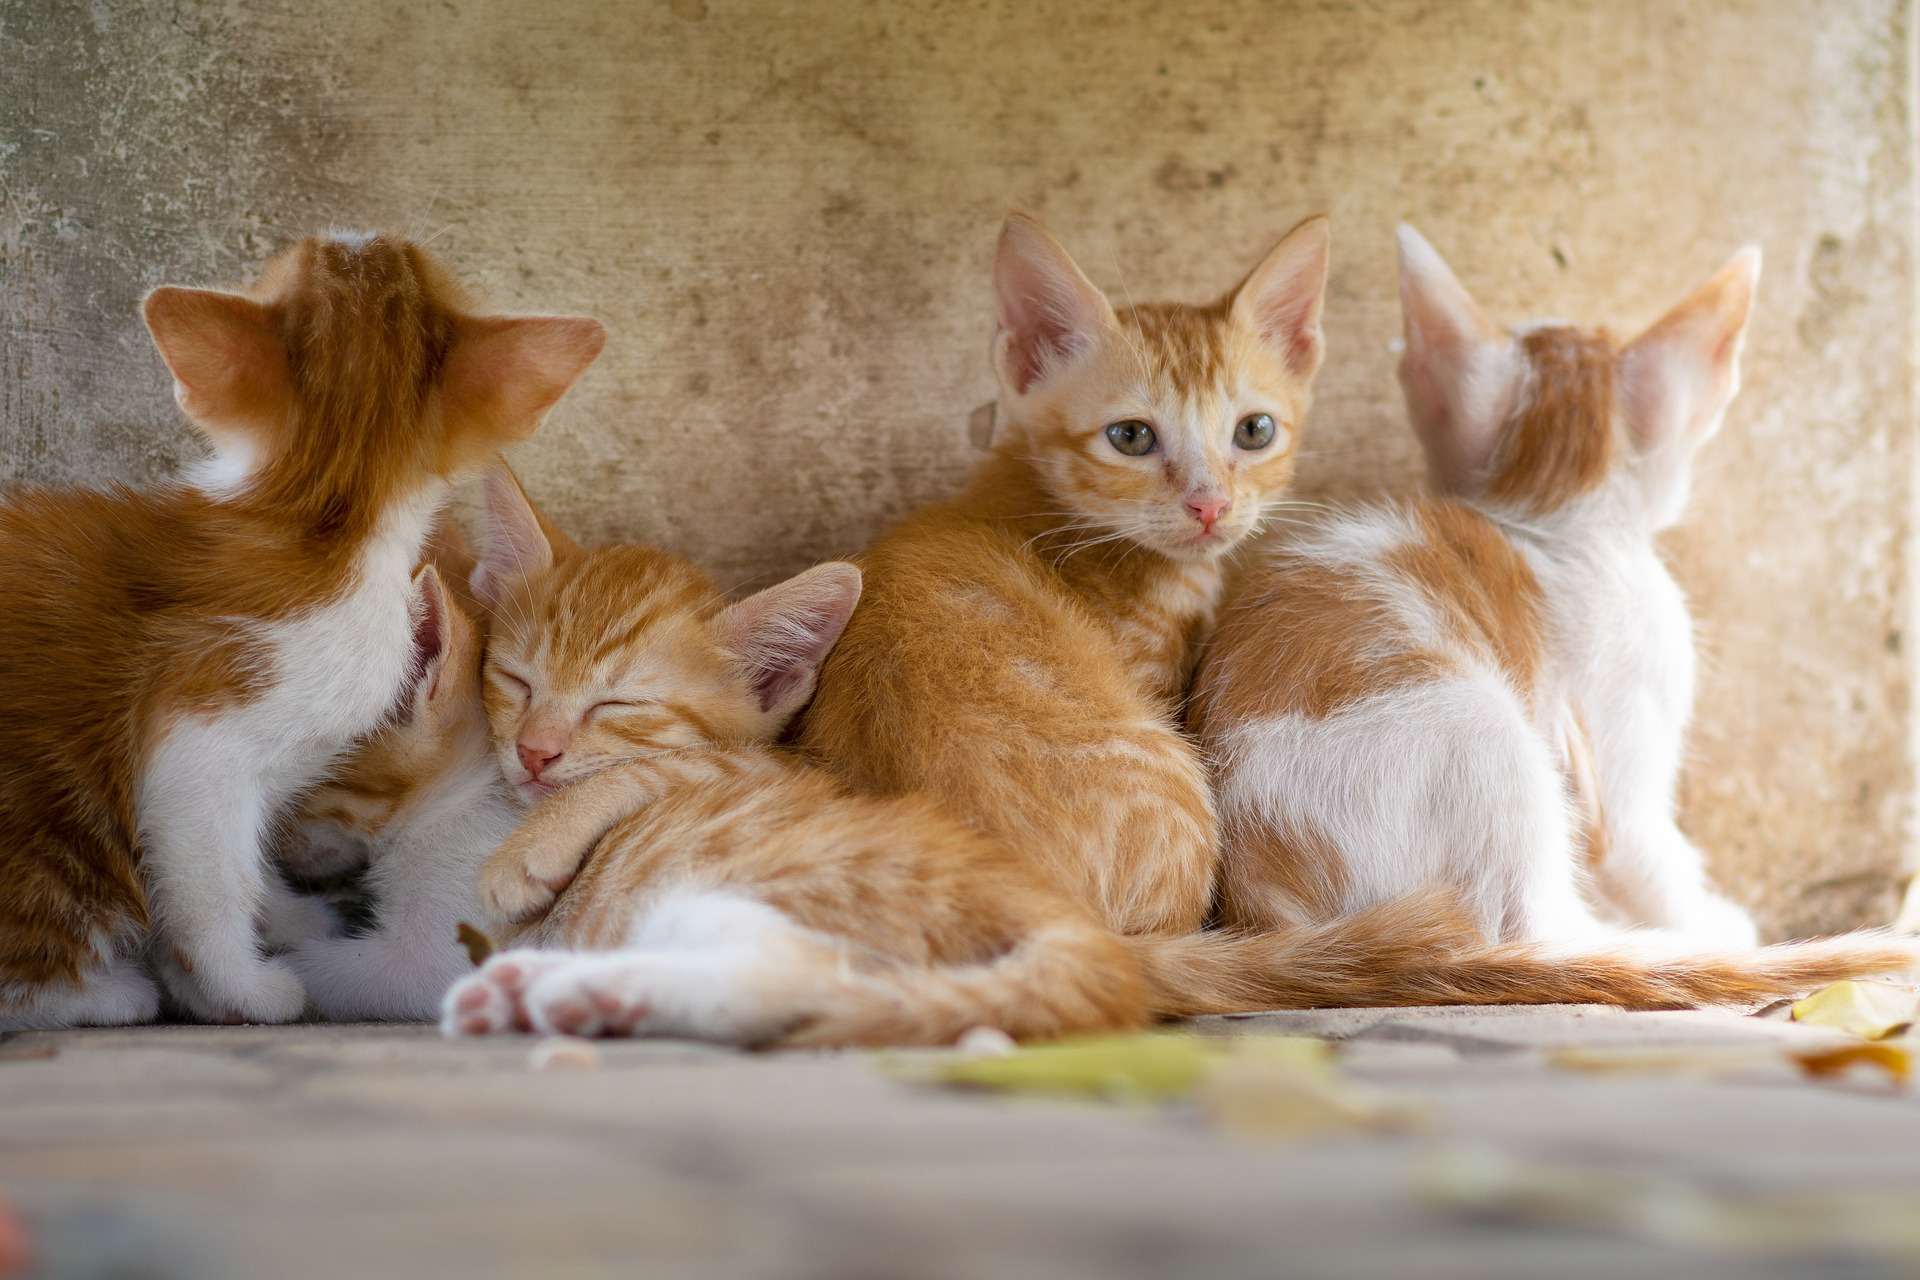
\includegraphics[width=11cm]{img/cats-pixabay01.jpg}
\caption{ ~\parencite{imageCats}}
\end{figure}
\begin{itemize}
 \item Visual Cortex ~\parencite{hubel1959receptive}
\end{itemize}
\end{frame}

\begin{frame}
\frametitle{}%{... and dogs}
\begin{figure}[h]
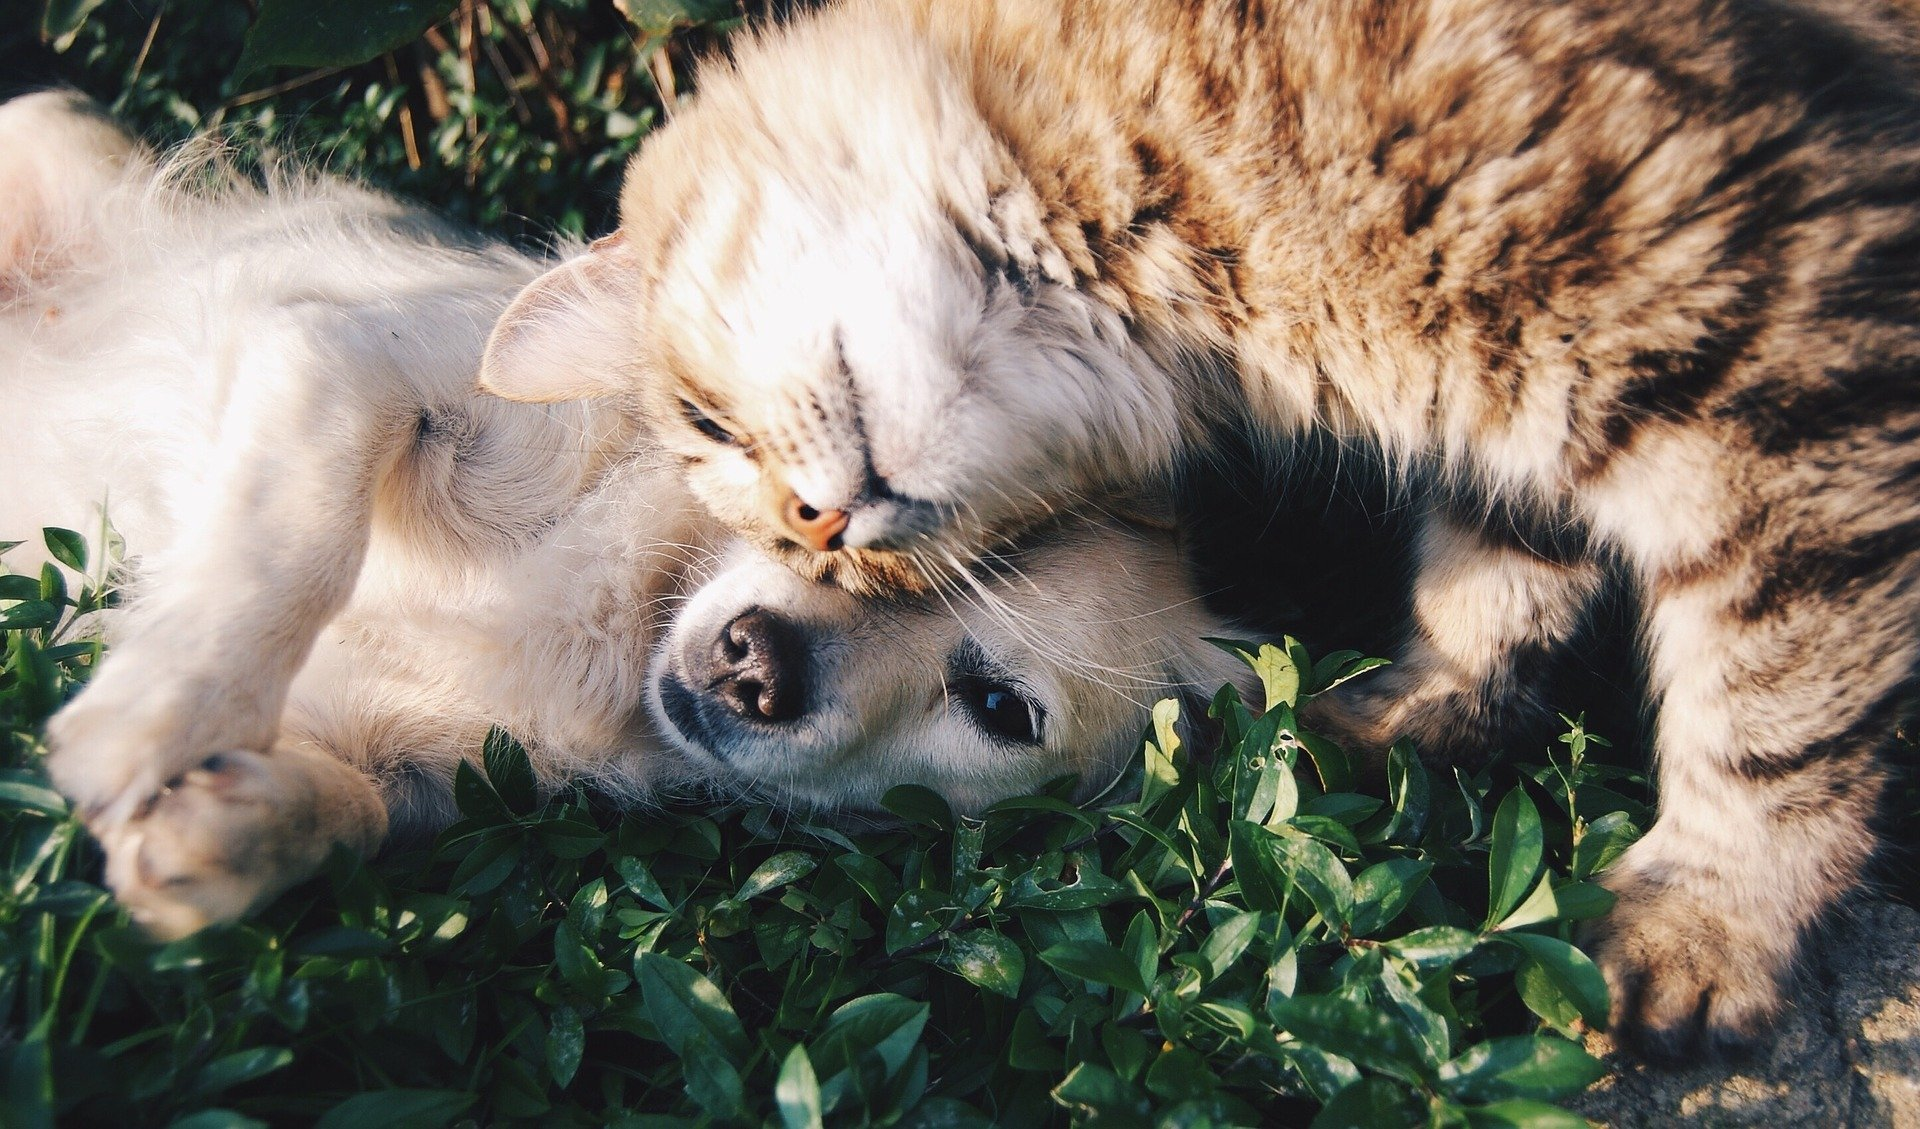
\includegraphics[width=11cm]{img/catDog-pixabay01.jpg}
\caption{ ~\parencite{imageCatDog}}
\end{figure}
\begin{itemize}
\item  AlexNet \& ImageNet~\parencite{krizhevsky2012imagenet}
\item CNN for object classification: cats vs. dogs 
\end{itemize}
\end{frame}


\begin{frame}
\frametitle{Engineering Tasks}%{... and dogs}
\begin{figure}[h]
\centering
\stackinset{r}{-.0\textwidth}{t}{-.10\textwidth}{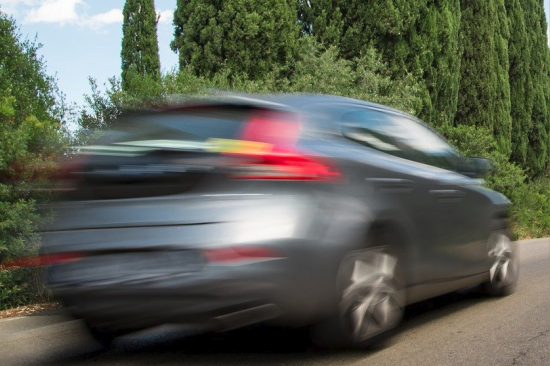
\includegraphics[width=0.35\textwidth,  trim = 0cm 0cm 0cm 0cm, clip]{img/car_speeding.png}}{%
%\stackinset{l}{+.00\textwidth}{t}{-.33\textwidth}{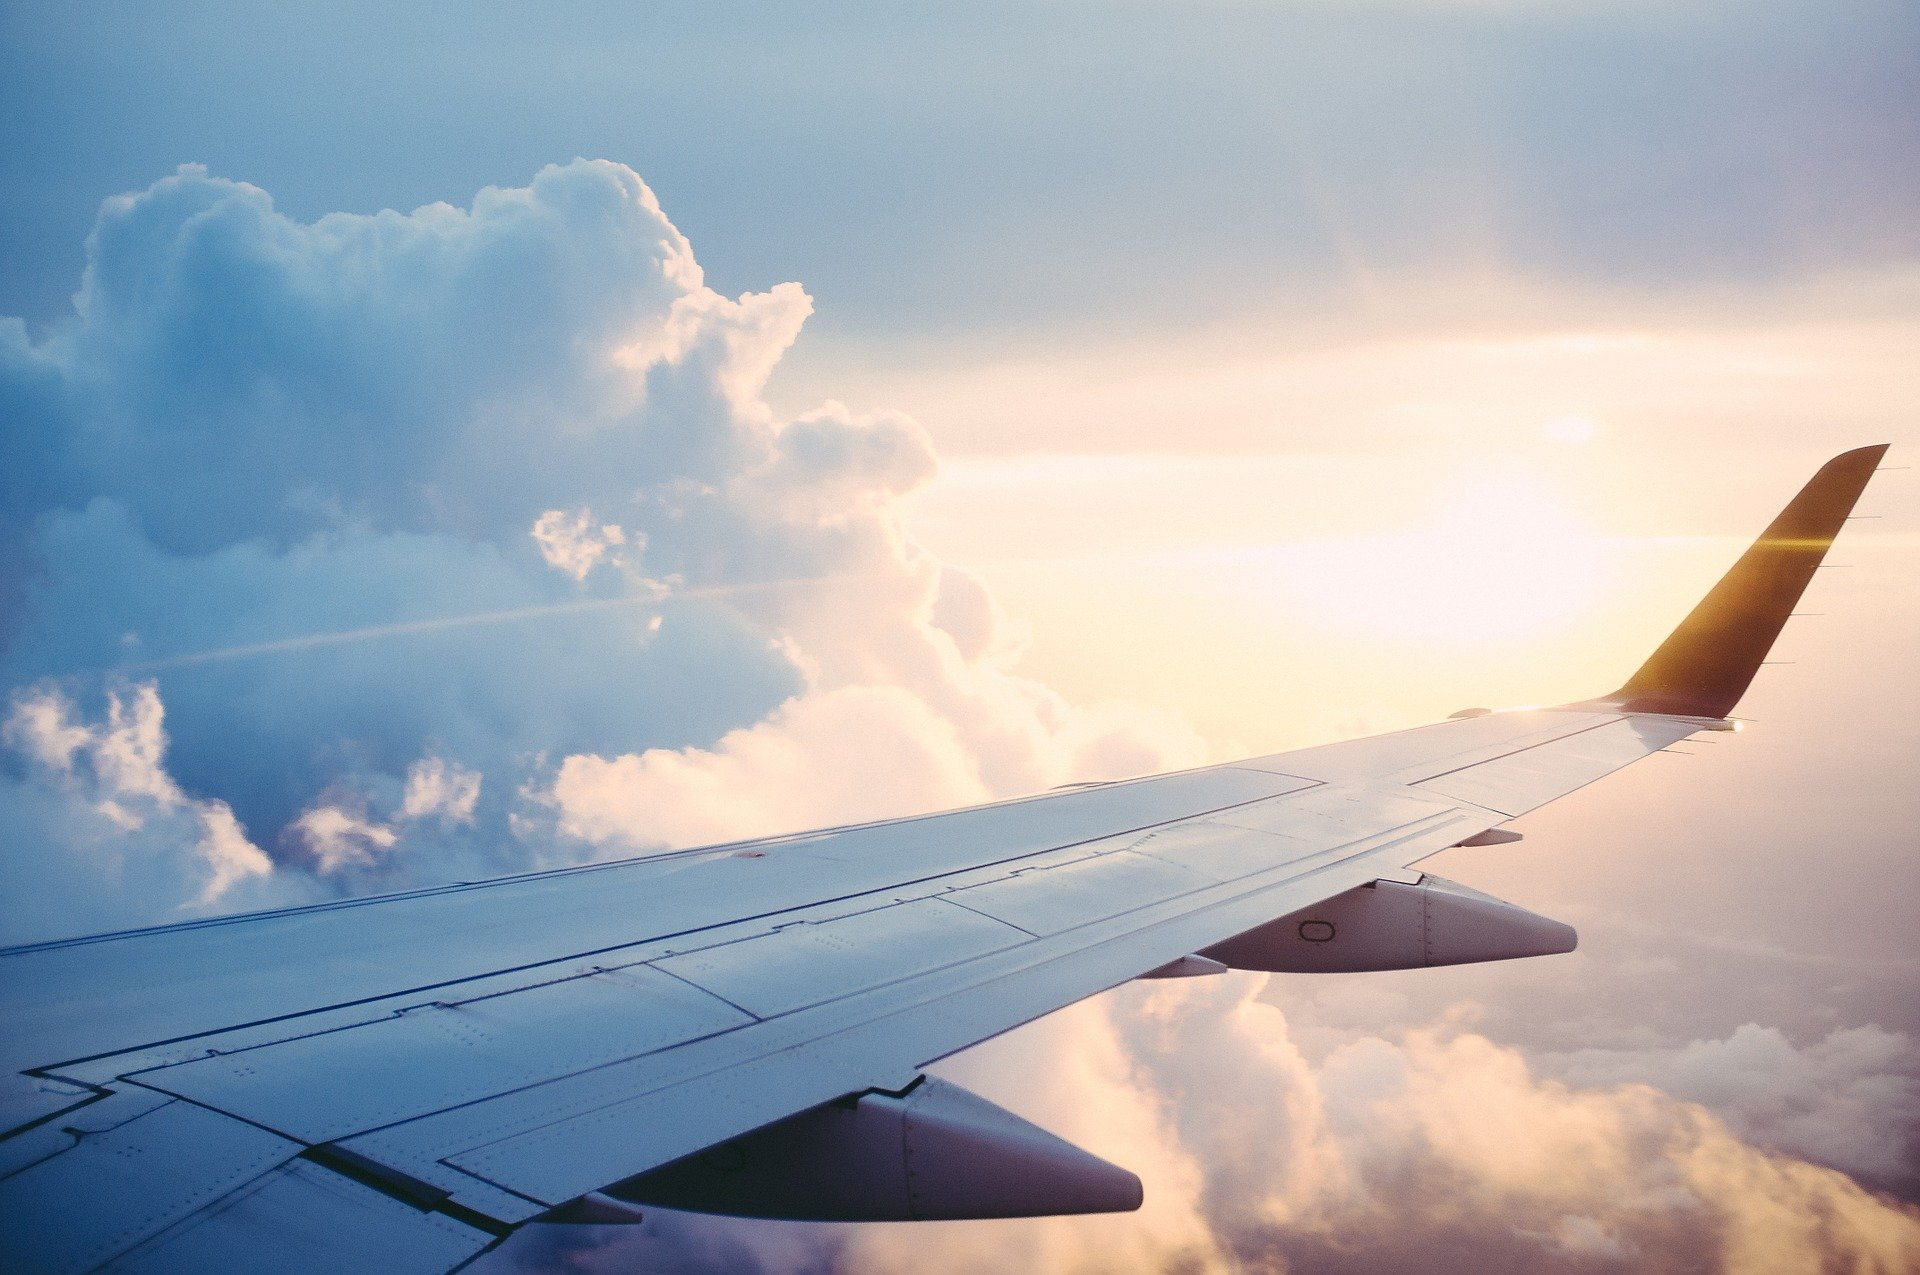
\includegraphics[width=0.6\textwidth, trim = 0cm 0cm 0cm 5cm, clip]{img/plane-841441_1920.jpg}}
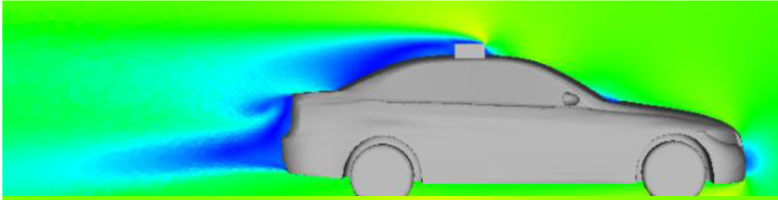
\includegraphics[width=1\textwidth, trim = 10cm 0cm 0cm 0cm, clip]{img/car_optimization.png}}%}
\caption{ ~\parencite{carSpeeding}}
\end{figure}
\end{frame}


\begin{frame}
\frametitle{Engineering Tasks}%{... and dogs}
\begin{figure}[h]
\centering
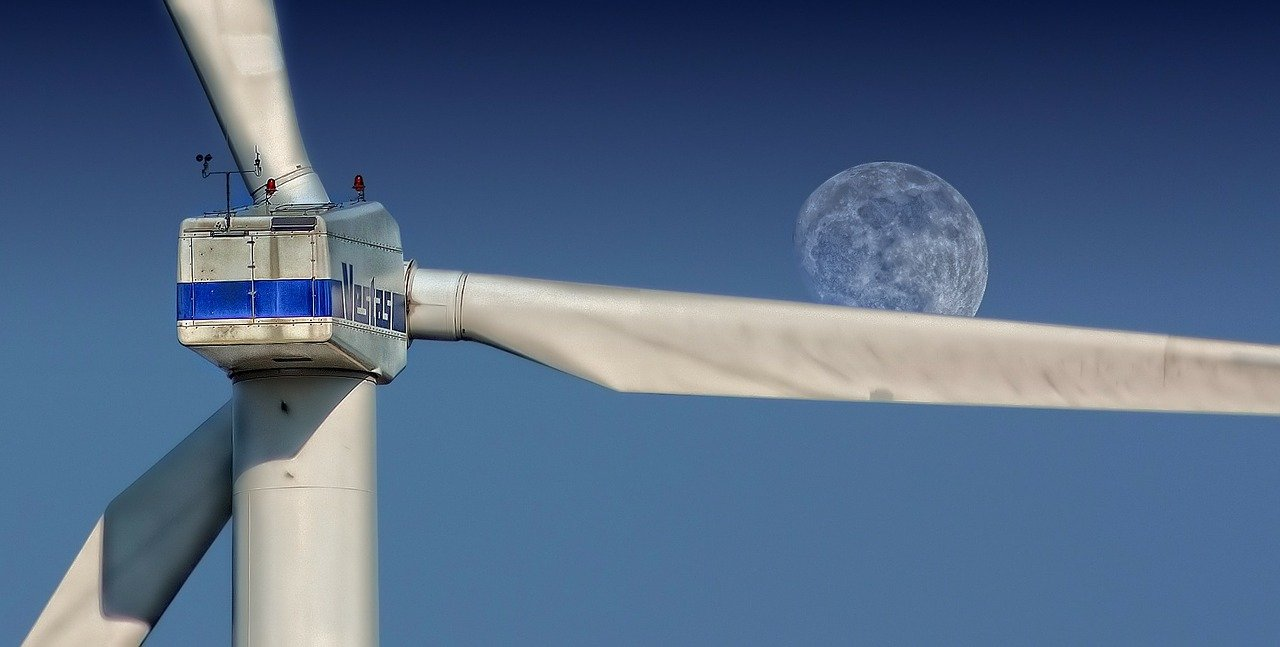
\includegraphics[width=0.5\textwidth, trim = 0cm 0cm 0cm 0cm, clip]{img/windmill-50512_1280.jpg}%

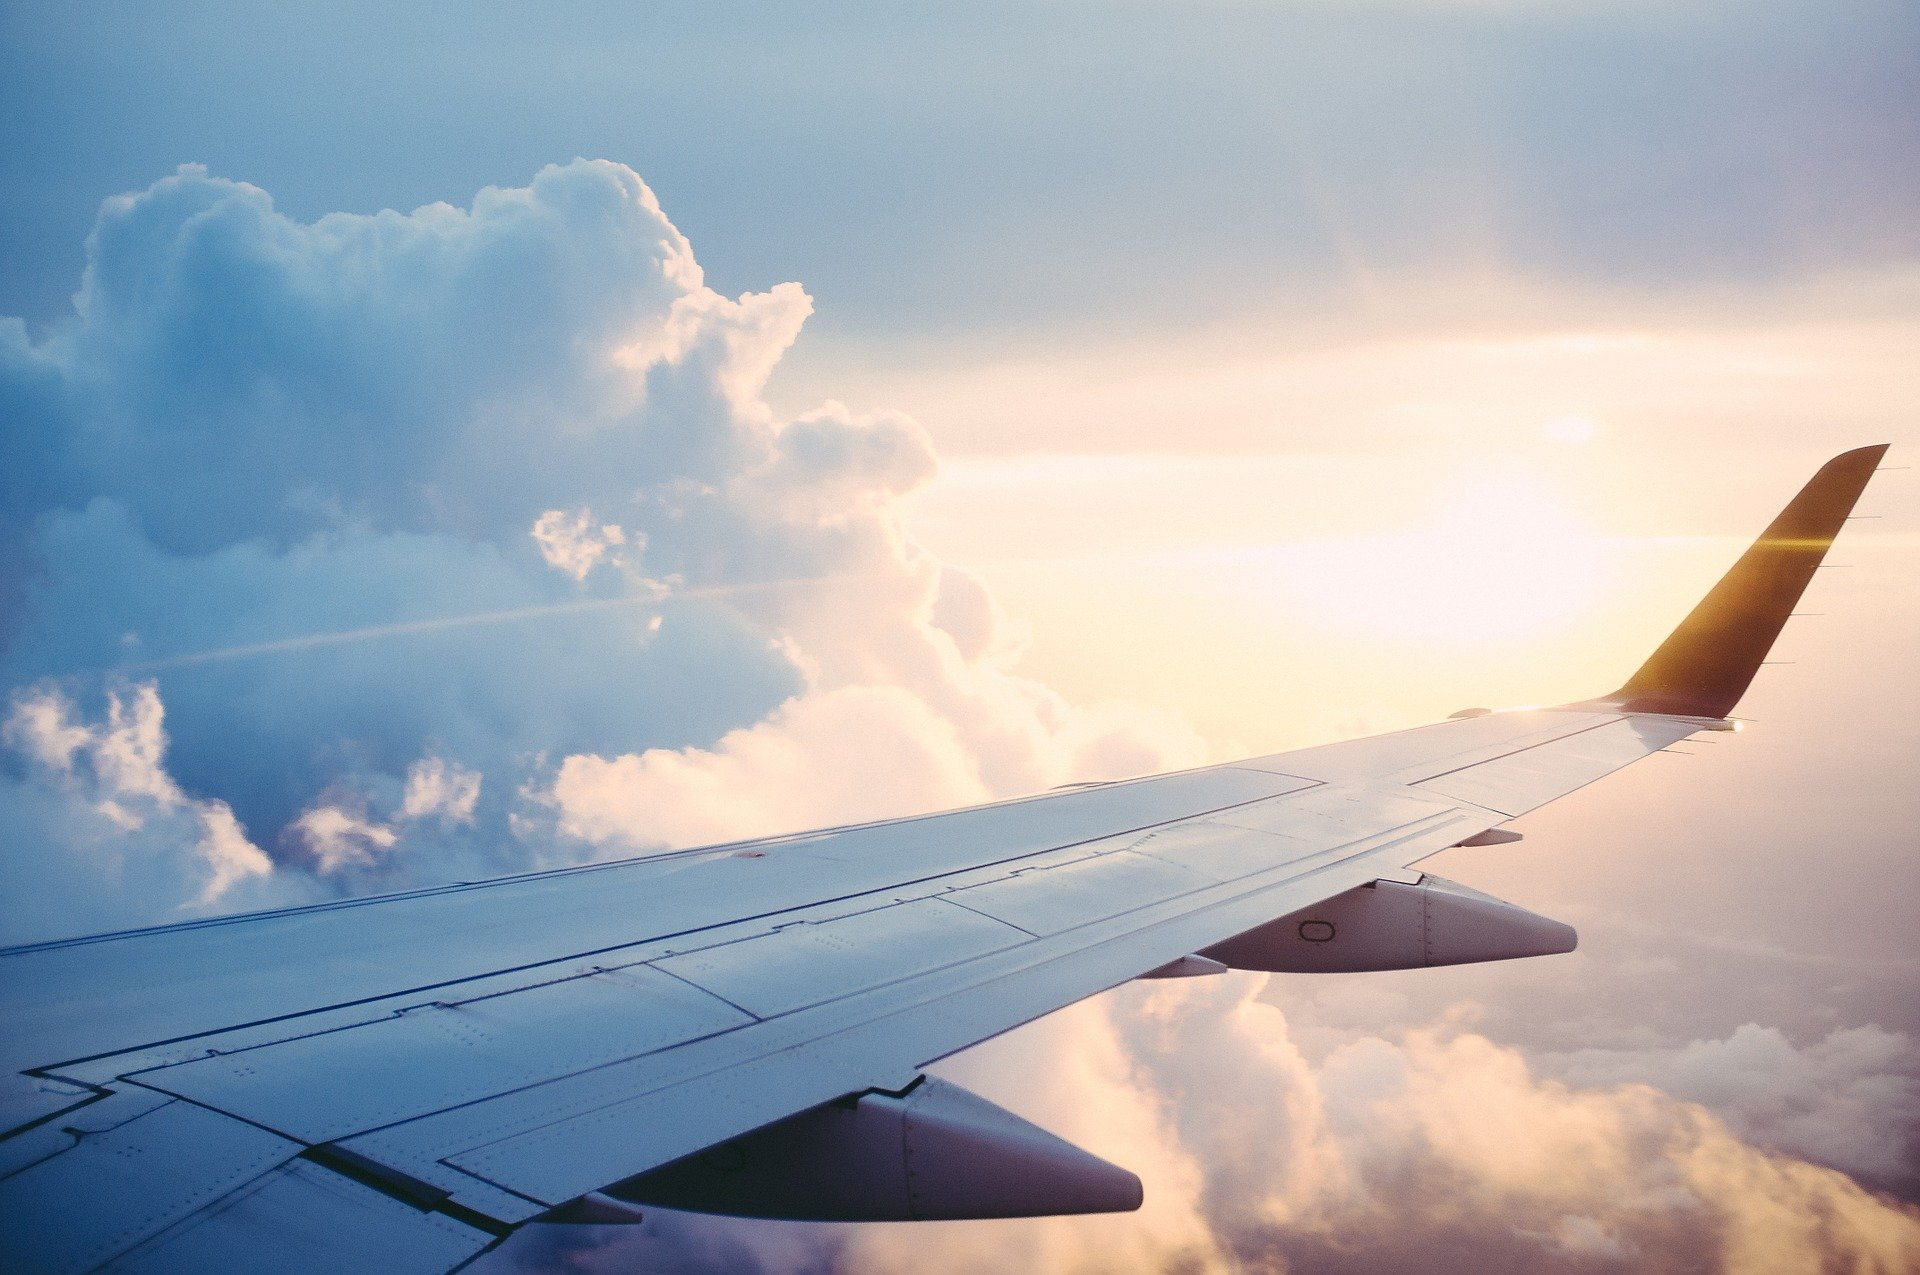
\includegraphics[width=0.5\textwidth, trim = 0cm 0cm 0cm 0cm, clip]{img/plane-841441_1920.jpg}%
\caption{ ~\parencite{windTurbines}}
\end{figure}
\end{frame}

\section{Patterns}
\begin{frame}
\frametitle{Patterns}
\begin{figure}[!ht]%
    \centering%
    \begin{minipage}{.48\textwidth}%
        \centering%
        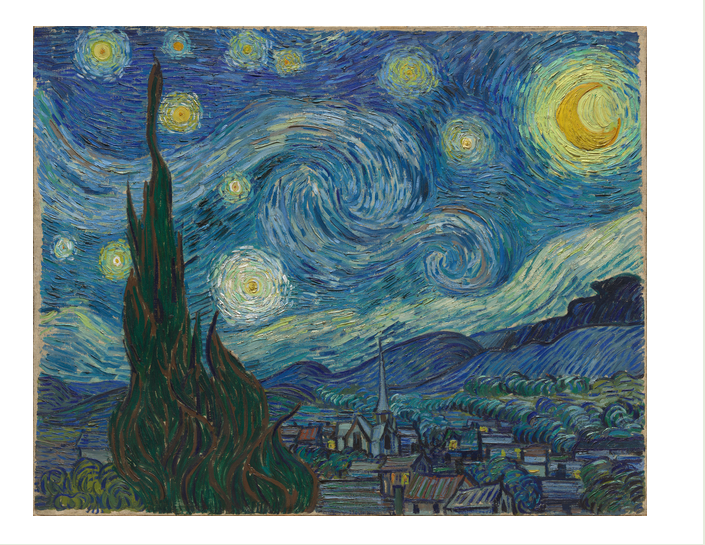
\includegraphics[height=0.72\linewidth, trim = 1.15cm 1.15cm 1.90cm 1.15cm, clip]{img/starryNight_vanGogh.png}%
        \caption{~\parencite{starryNight}}%Turbulence Patterns
        \label{fig:prob1_6_2}%
    \end{minipage}%
    \begin{minipage}{0.50\textwidth}%
        \centering%
        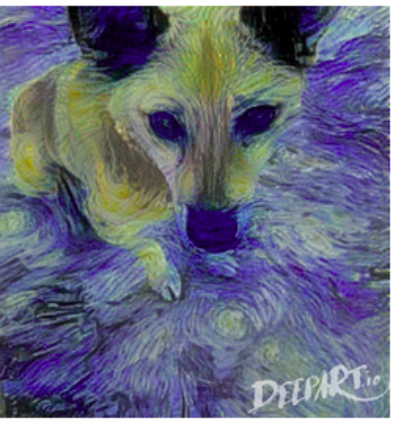
\includegraphics[height=0.75\linewidth]{img/cucio_starryNight_vanGogh.png}
        \caption{\tiny{Neural Style Transfer} ~\parencite{gatys2016image}}%
        \label{fig:prob1_6_1}%
    \end{minipage}%
\end{figure}
\end{frame}


\begin{frame}
\frametitle{Patterns in Turbulent Flows}
\begin{figure}[h]
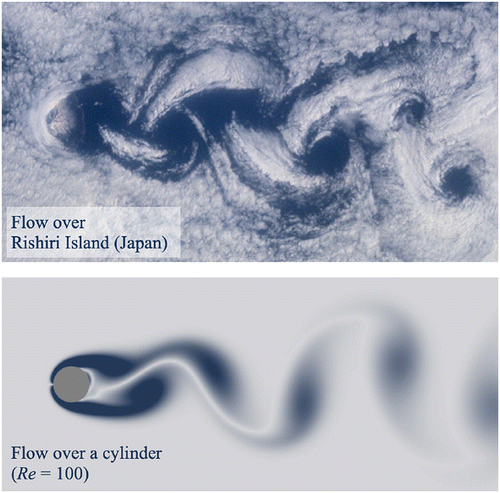
\includegraphics[width=7cm]{img/flow_over_rishiri_island.png}
\caption{\tiny{} ~\parencite{taira2020modal}}
%The von Kármán vortex street generated by the Rishiri island of Hokkaido, Japan (top, photo from NASA, 2001; STS-100). This wake produced at high Reynolds number shares great similarity with the cylinder wake at low Reynolds number (bottom).
\end{figure}
\end{frame}

\begin{frame}
\frametitle{Patterns in Turbulent Flows}
\begin{figure}[!htb]%
    \centering%
    \begin{minipage}{.5\textwidth}%
        \centering%
        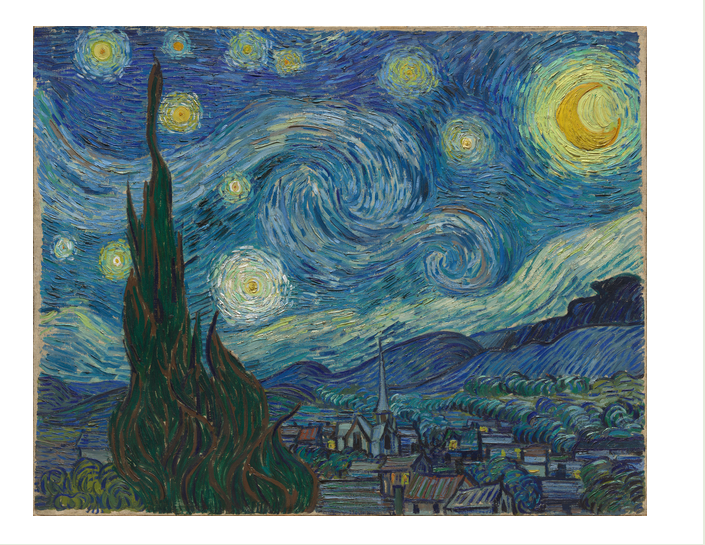
\includegraphics[height=0.72\linewidth, trim = 1.15cm 1.15cm 1.90cm 1.15cm, clip]{img/starryNight_vanGogh.png}%
        \caption{\tiny{Turbulent luminance in impassioned van Gogh paintings} ~\parencite{aragon2008turbulent}}%
        \label{fig:prob1_6_2}%
    \end{minipage}%
    \begin{minipage}{0.5\textwidth}%
        \centering%
        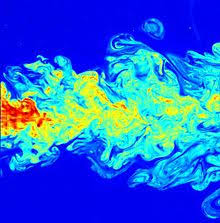
\includegraphics[height=0.72\linewidth]{img/energyCasacade.jpeg}
        \caption{\tiny{Turbulence jet  with wide range of length scales}, ~\parencite{energyCascade}}%
        %Flow visualization of a turbulent jet, made by laser-induced fluorescence. The jet exhibits a wide range of length scales, a prerequisite for the appearance of an energy cascade in the turbulence modelling.
        \label{fig:prob1_6_1}%
    \end{minipage}%
\end{figure}
\end{frame}



\section{CFD Problem} % A subsection can be created just before a set of slides with a common theme to further break down your presentation into chunks
\begin{frame}
\frametitle{CFD Problem}
\begin{figure}[h]
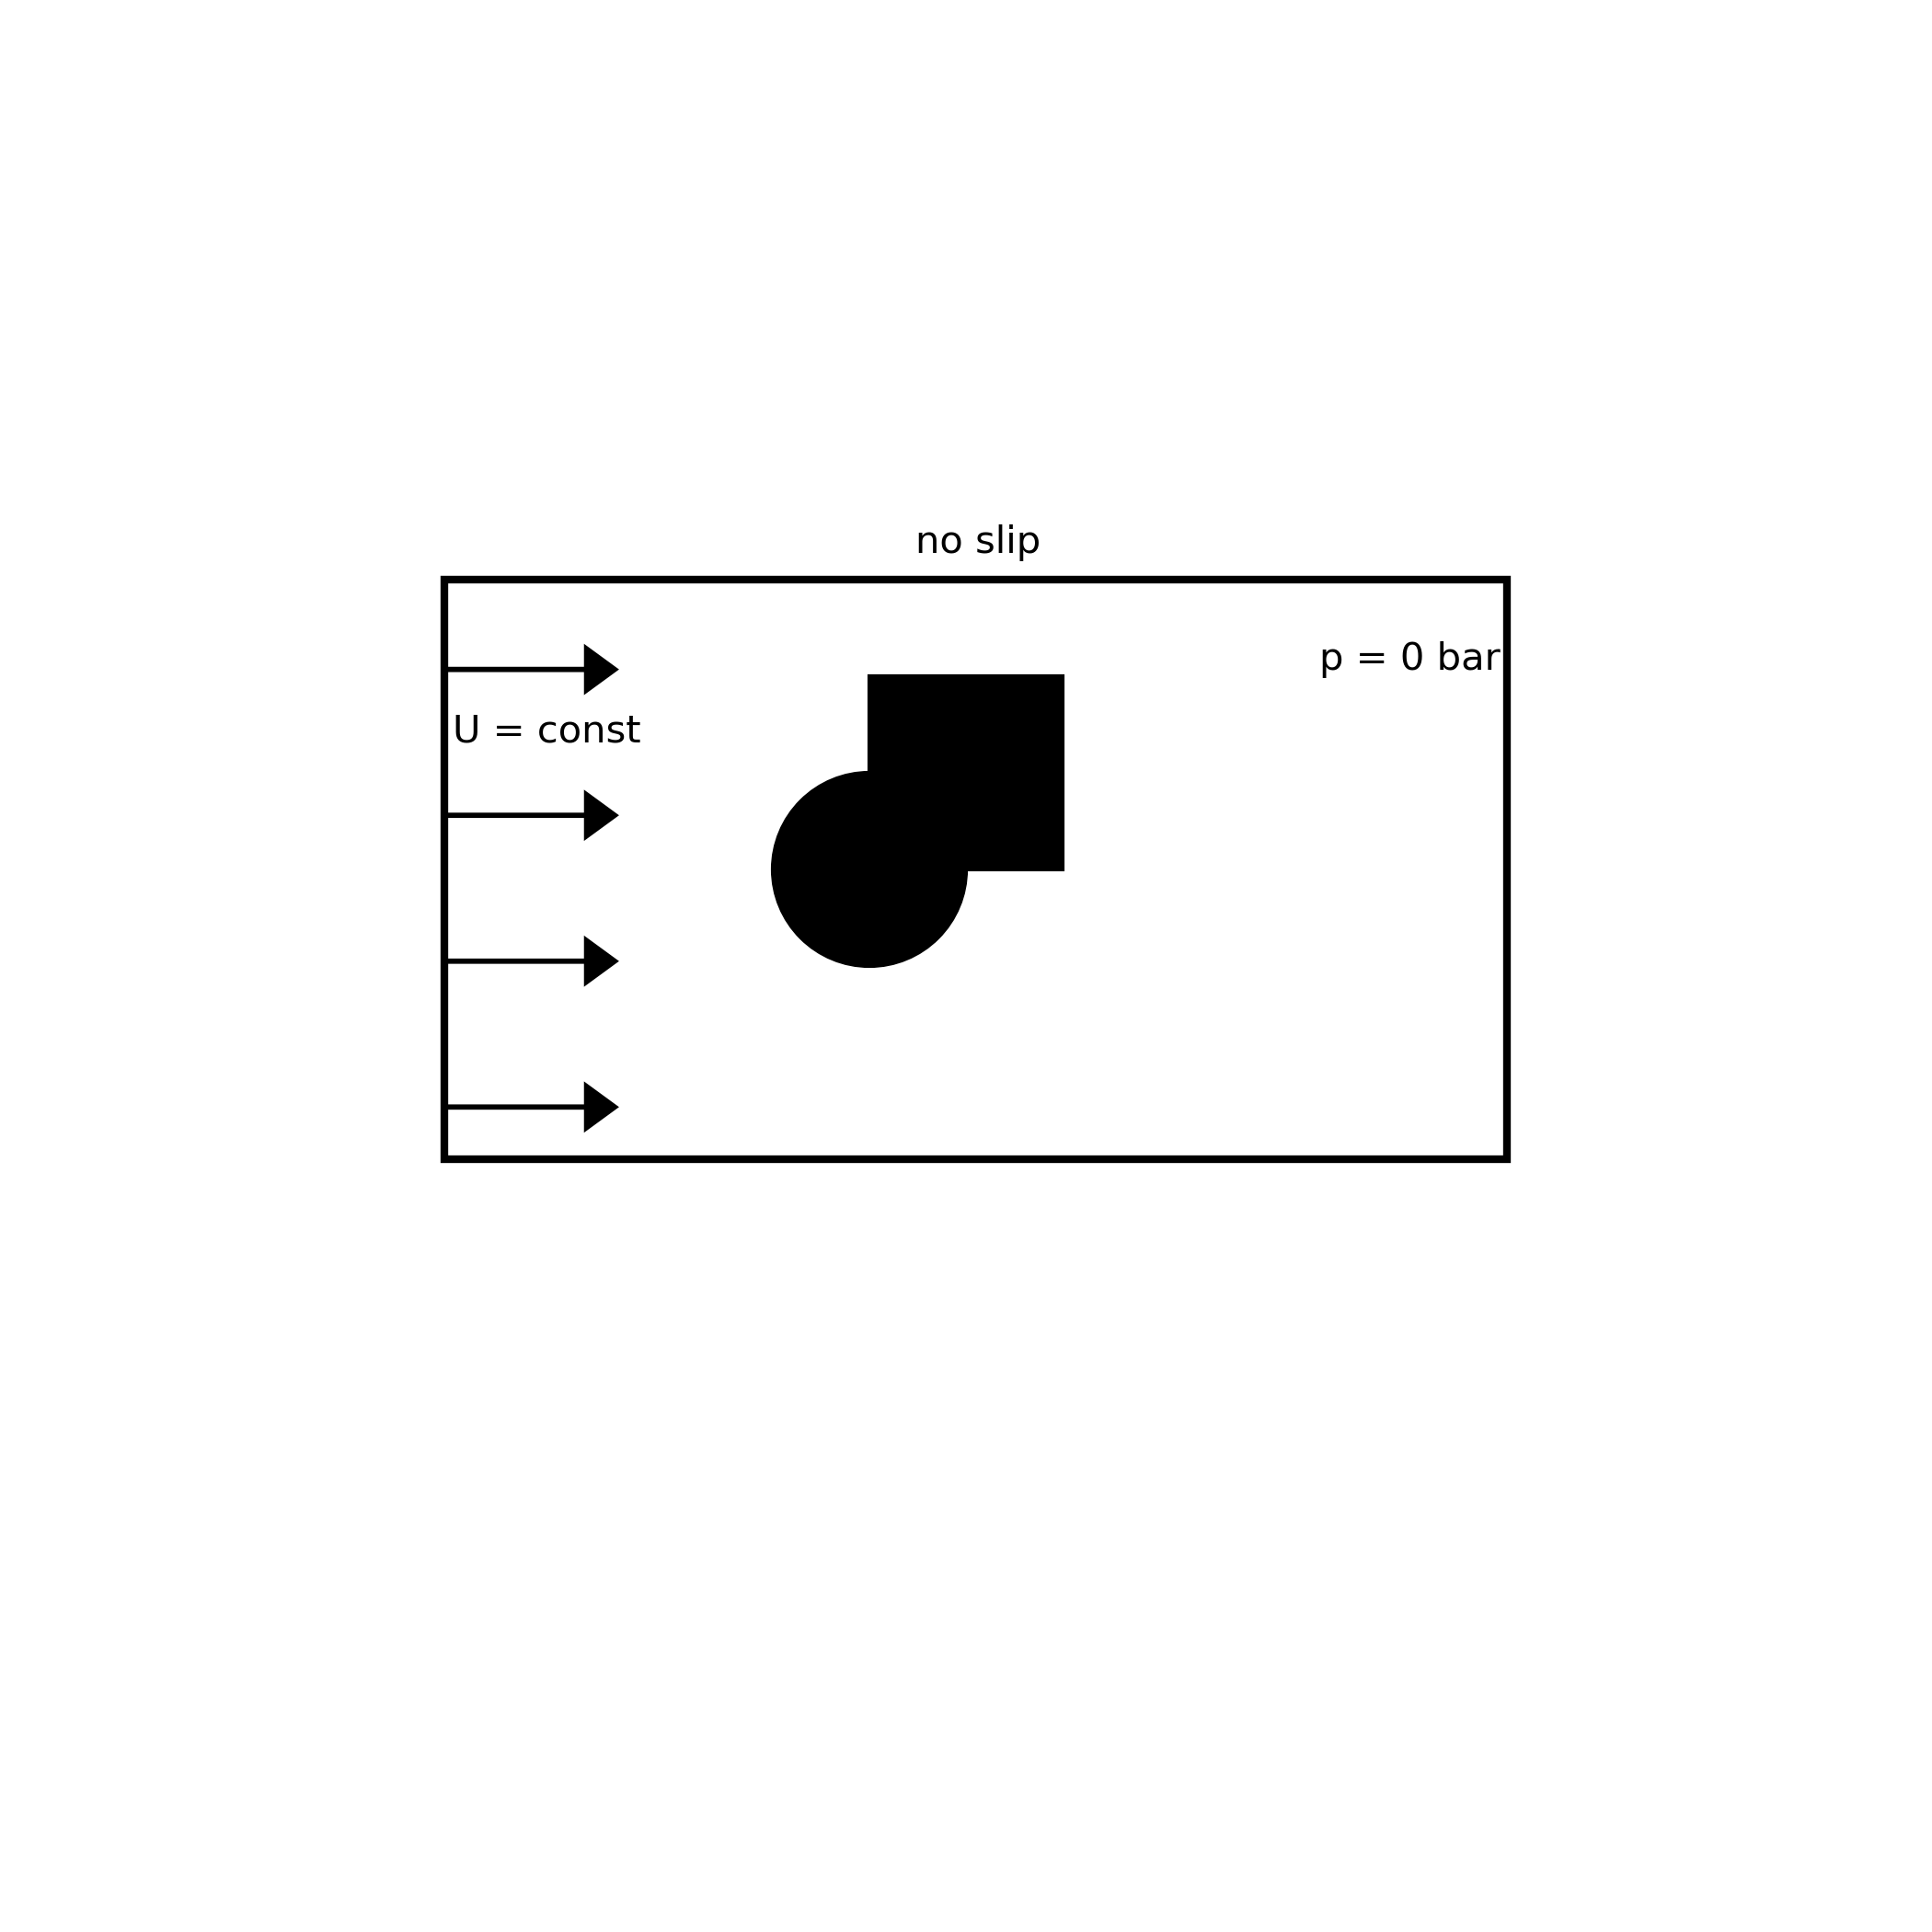
\includegraphics[width=9cm, trim = 3.9cm 6cm 3.5cm 4.5cm, clip]{img/BCs.png}
%\caption{Initial \& Boundary Conditions}
\end{figure}
\end{frame}





\begin{frame}
\frametitle{Train Data: random shape variations}
\begin{figure}[h]
%
\includegraphics[width=8cm, trim = 2cm 2cm 1cm 2cm, clip]{img/shapes.png}
%\caption{Geometry: shape variations generated randomly}
\vspace{0.4cm}
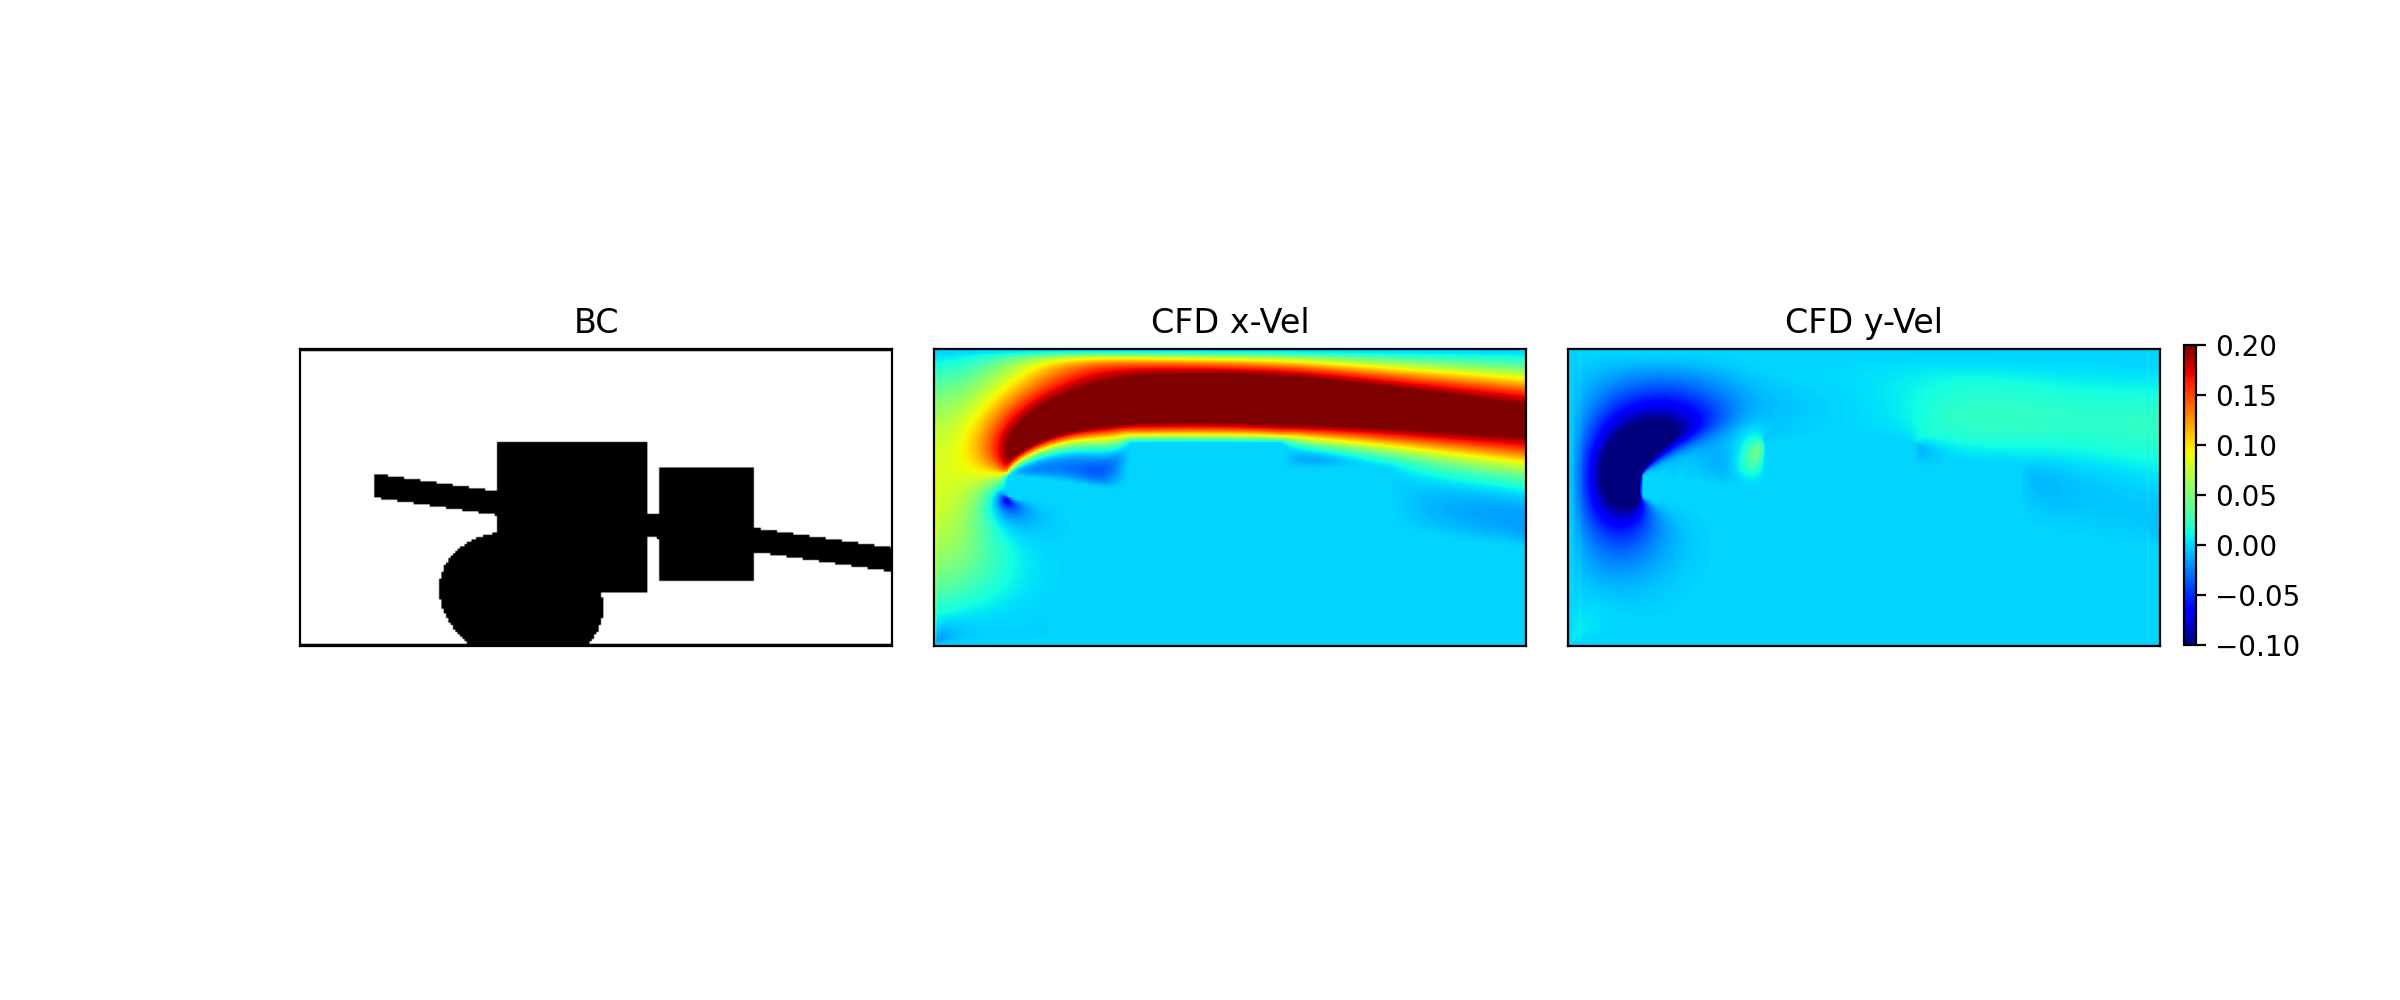
\includegraphics[height=0.16\linewidth, trim = 3.680cm 4.35cm 18.98cm 4.29cm, clip]{../../../plots/plots/train_data/montage_train_data_01.png}%      
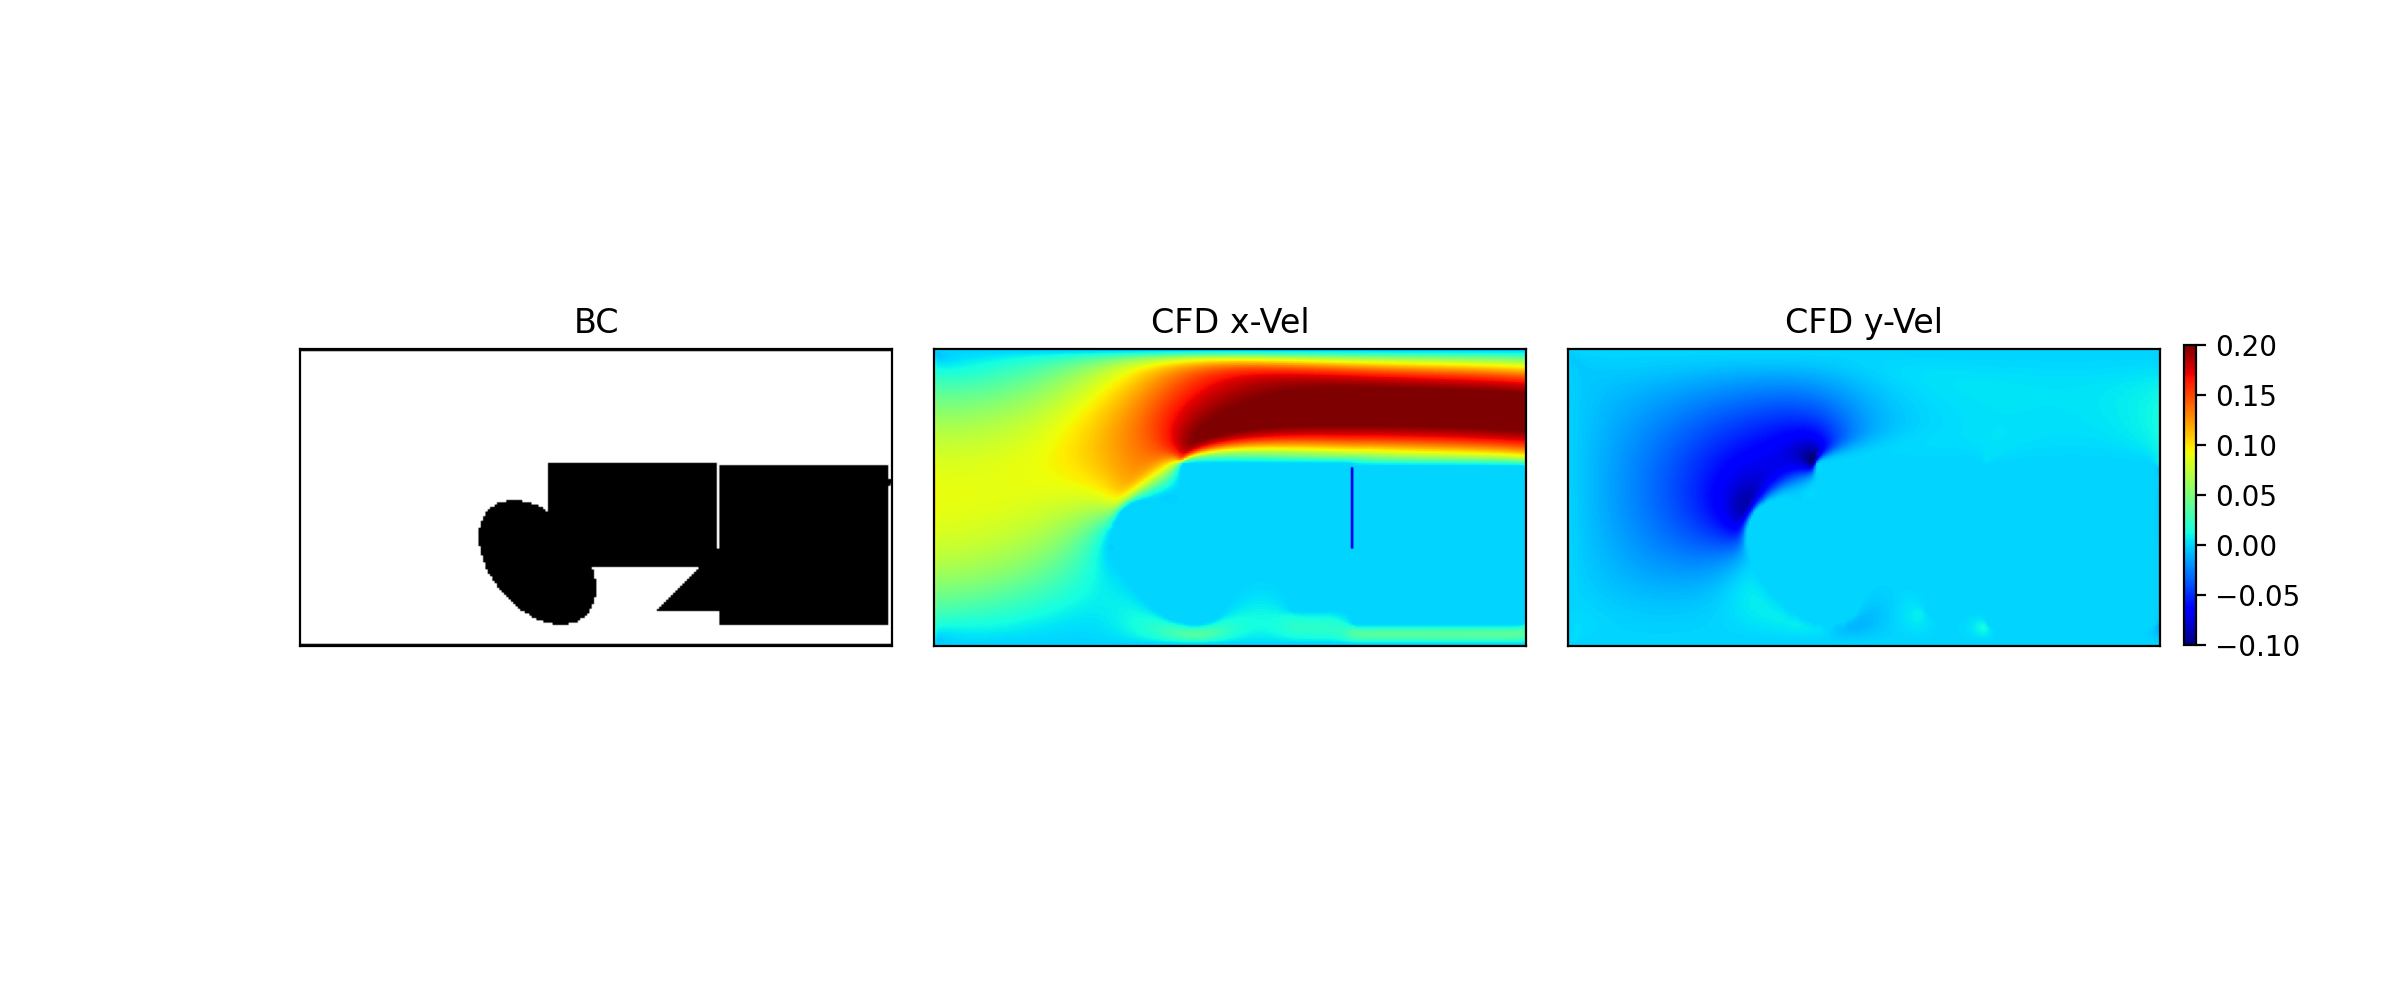
\includegraphics[height=0.16\linewidth, trim = 3.680cm 4.35cm 18.98cm 4.29cm, clip]{../../../plots/plots/train_data/montage_train_data_02.png}%
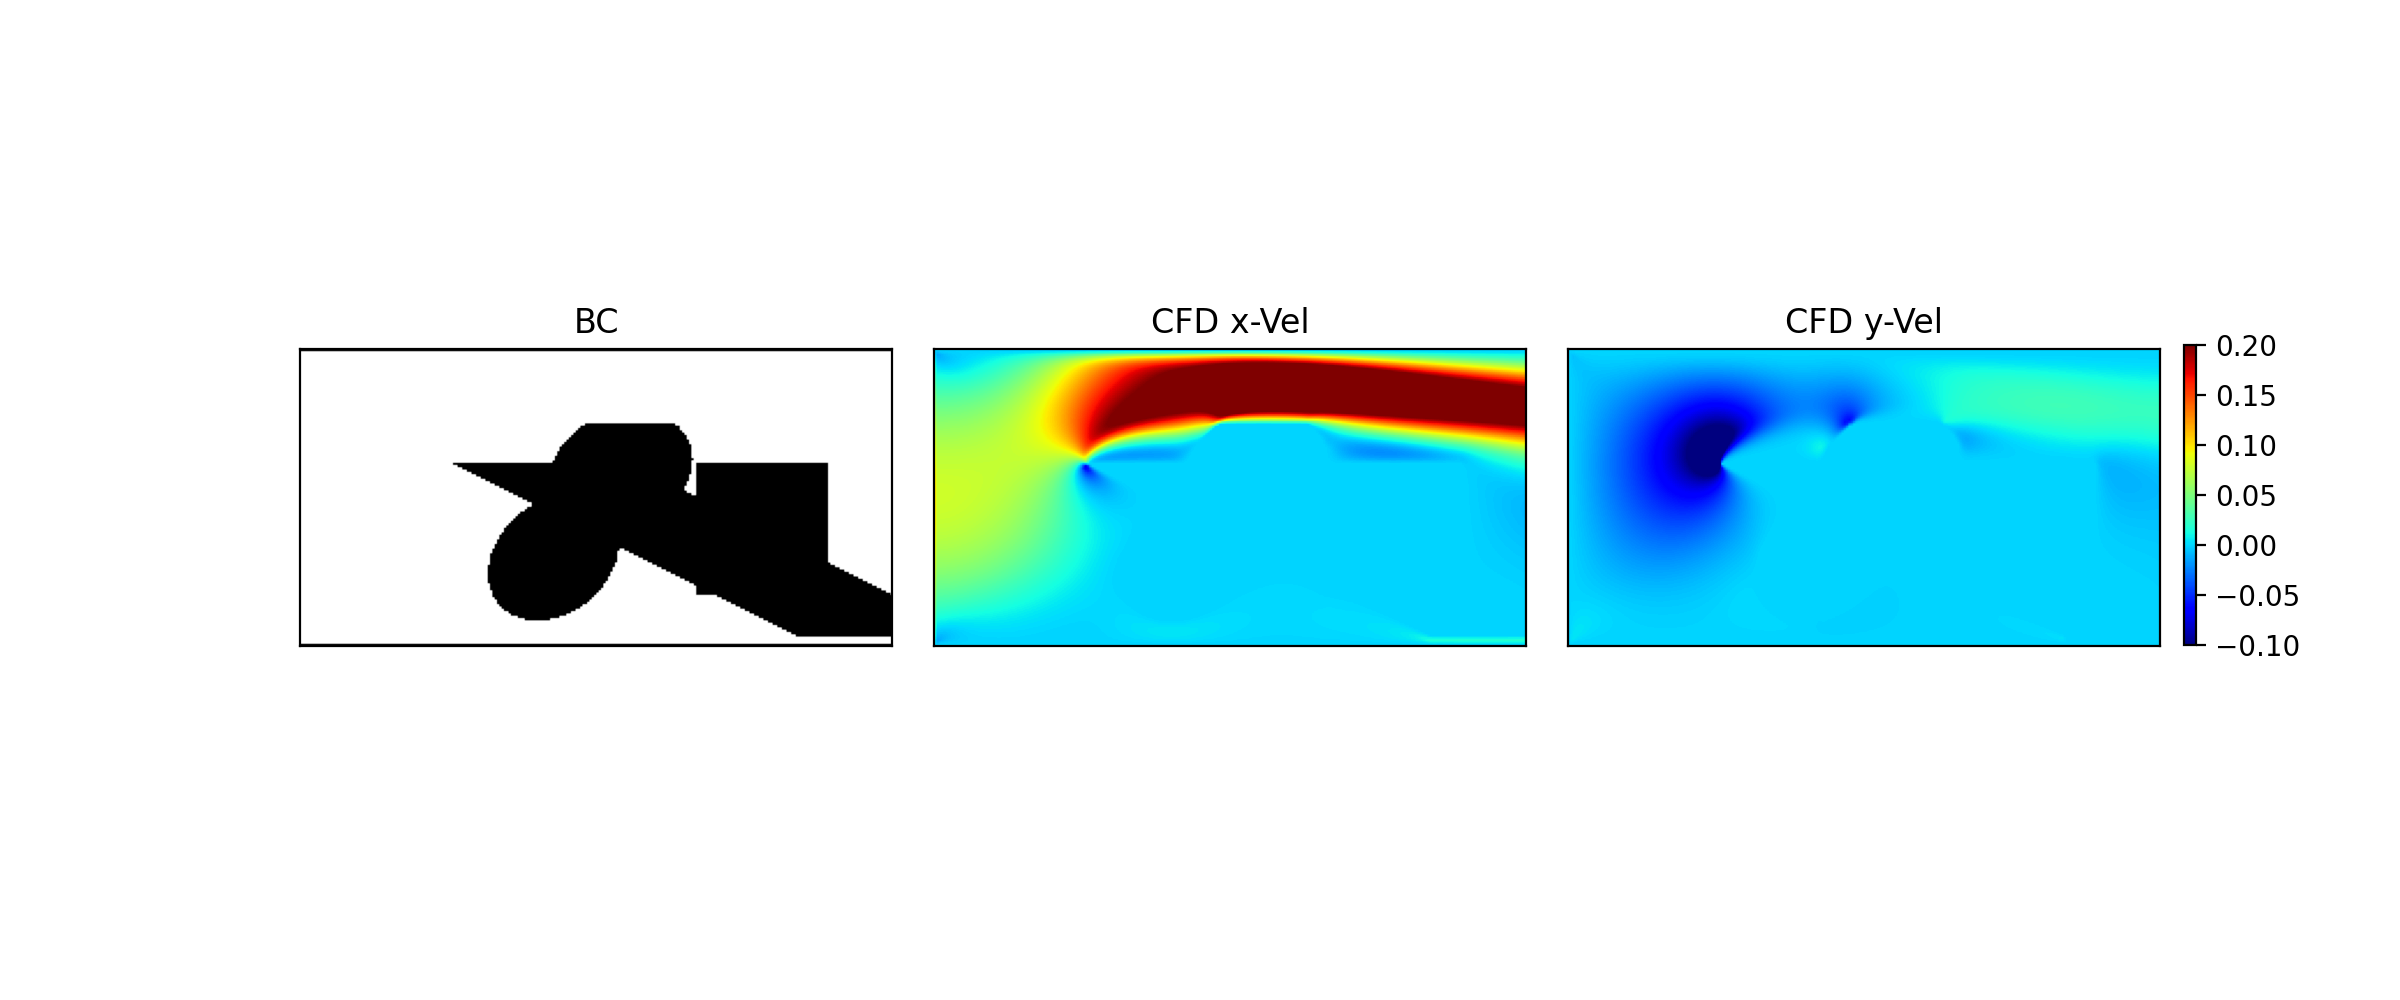
\includegraphics[height=0.16\linewidth, trim = 3.680cm 4.35cm 18.98cm 4.29cm, clip]{../../../plots/plots/train_data/montage_train_data_03.png}%

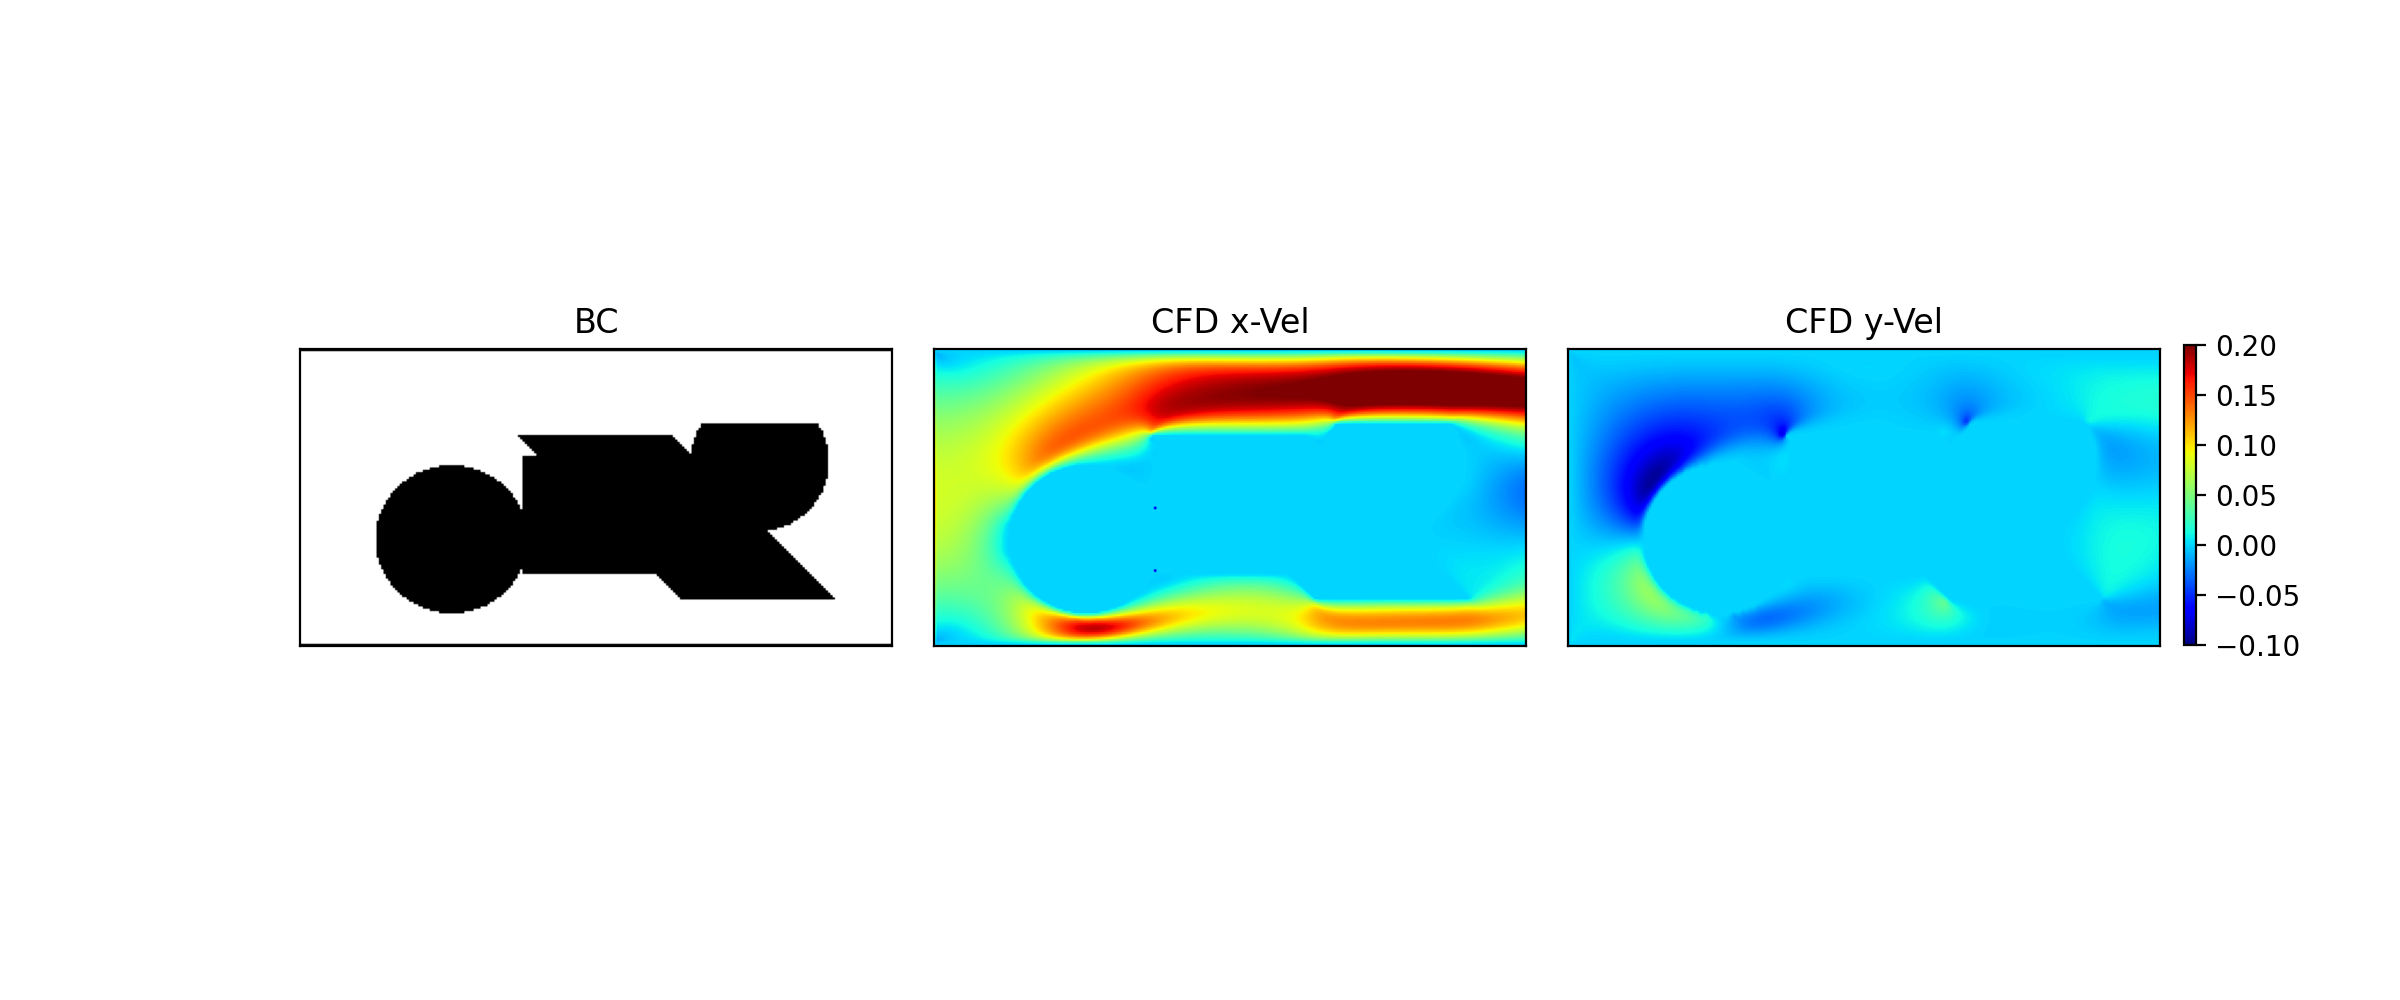
\includegraphics[height=0.16\linewidth, trim = 3.680cm 4.35cm 18.98cm 4.29cm, clip]{../../../plots/plots/train_data/montage_train_data_04.png}%     
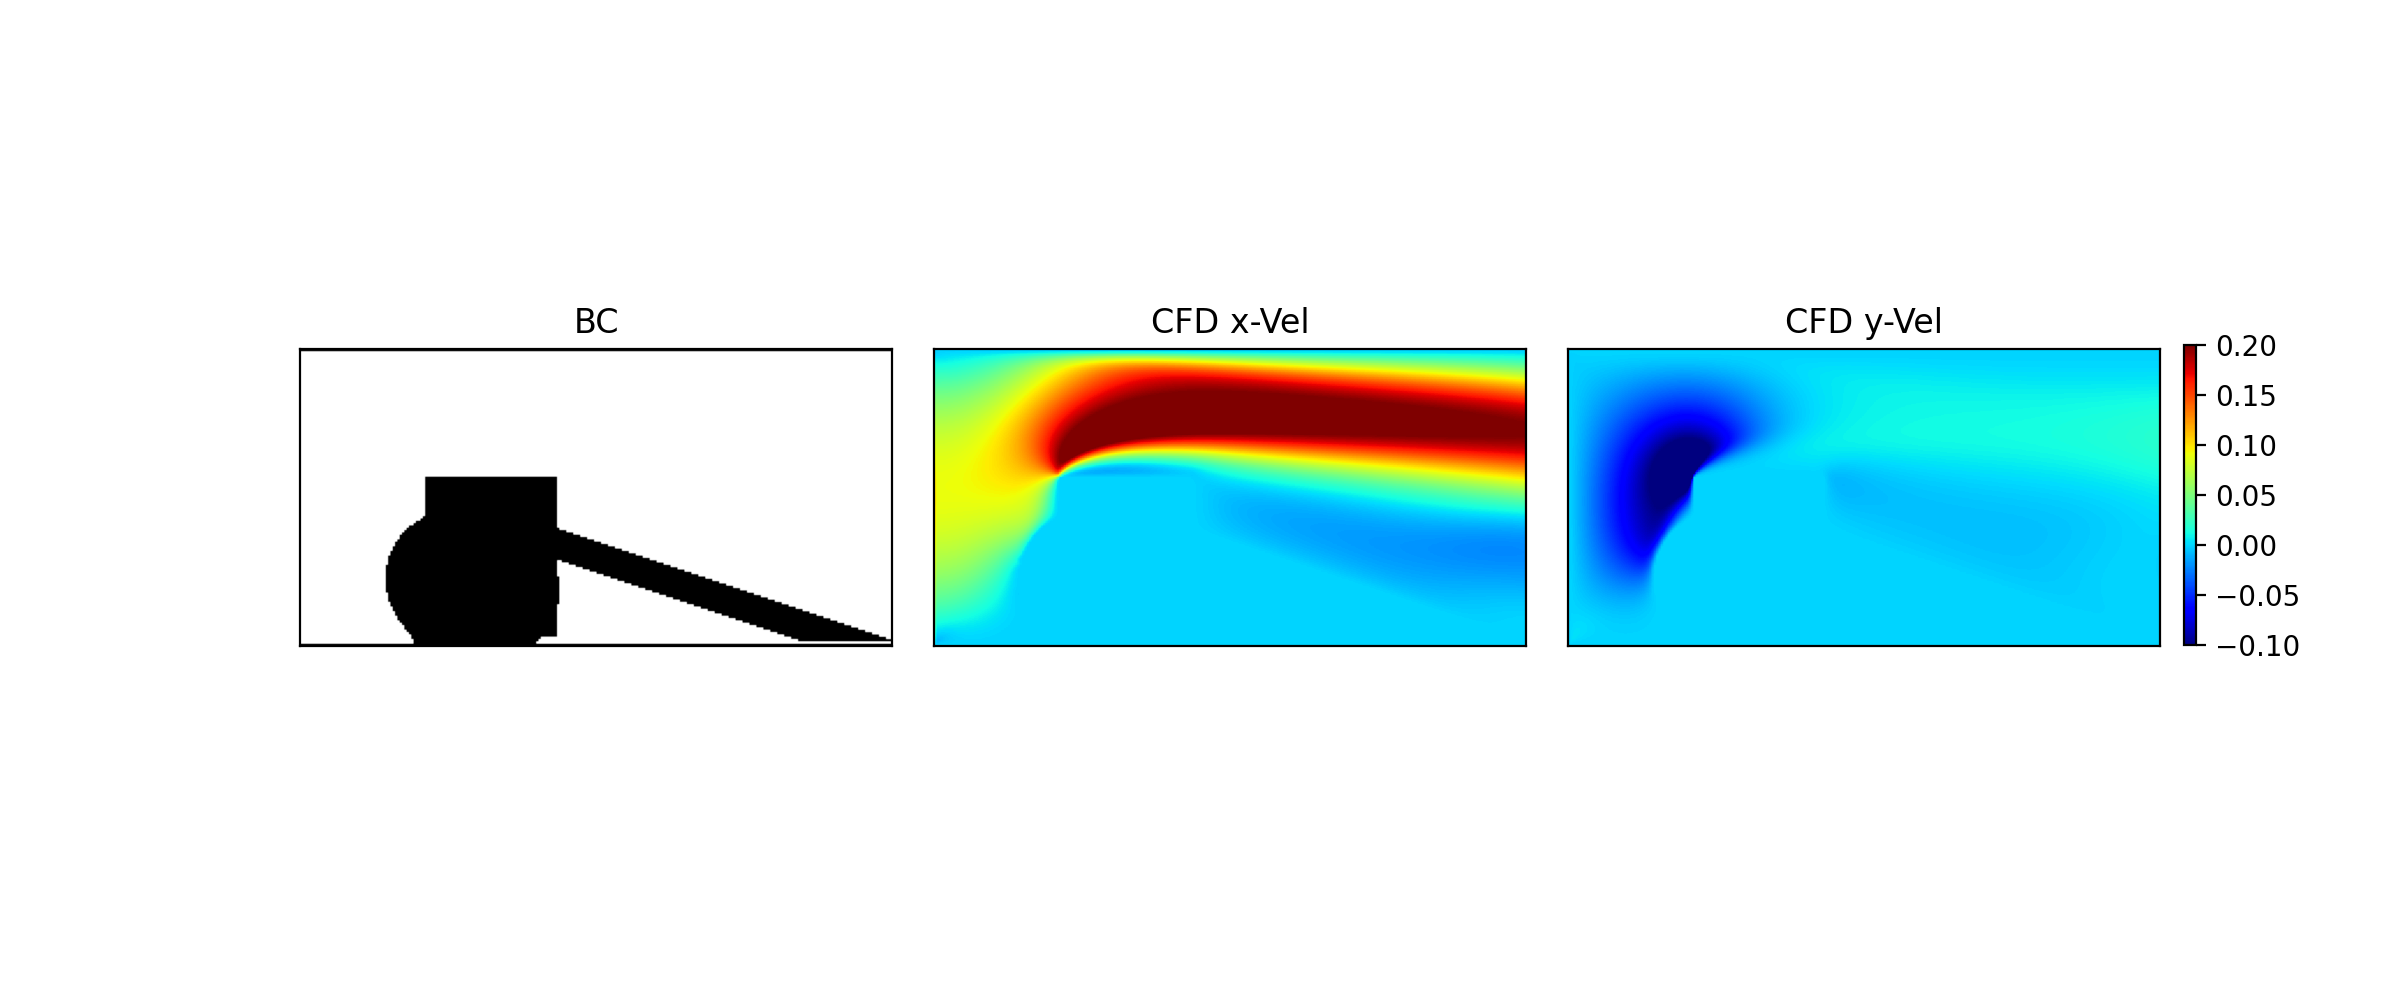
\includegraphics[height=0.16\linewidth, trim = 3.680cm 4.35cm 18.98cm 4.29cm, clip]{../../../plots/plots/train_data/montage_train_data_05.png}%
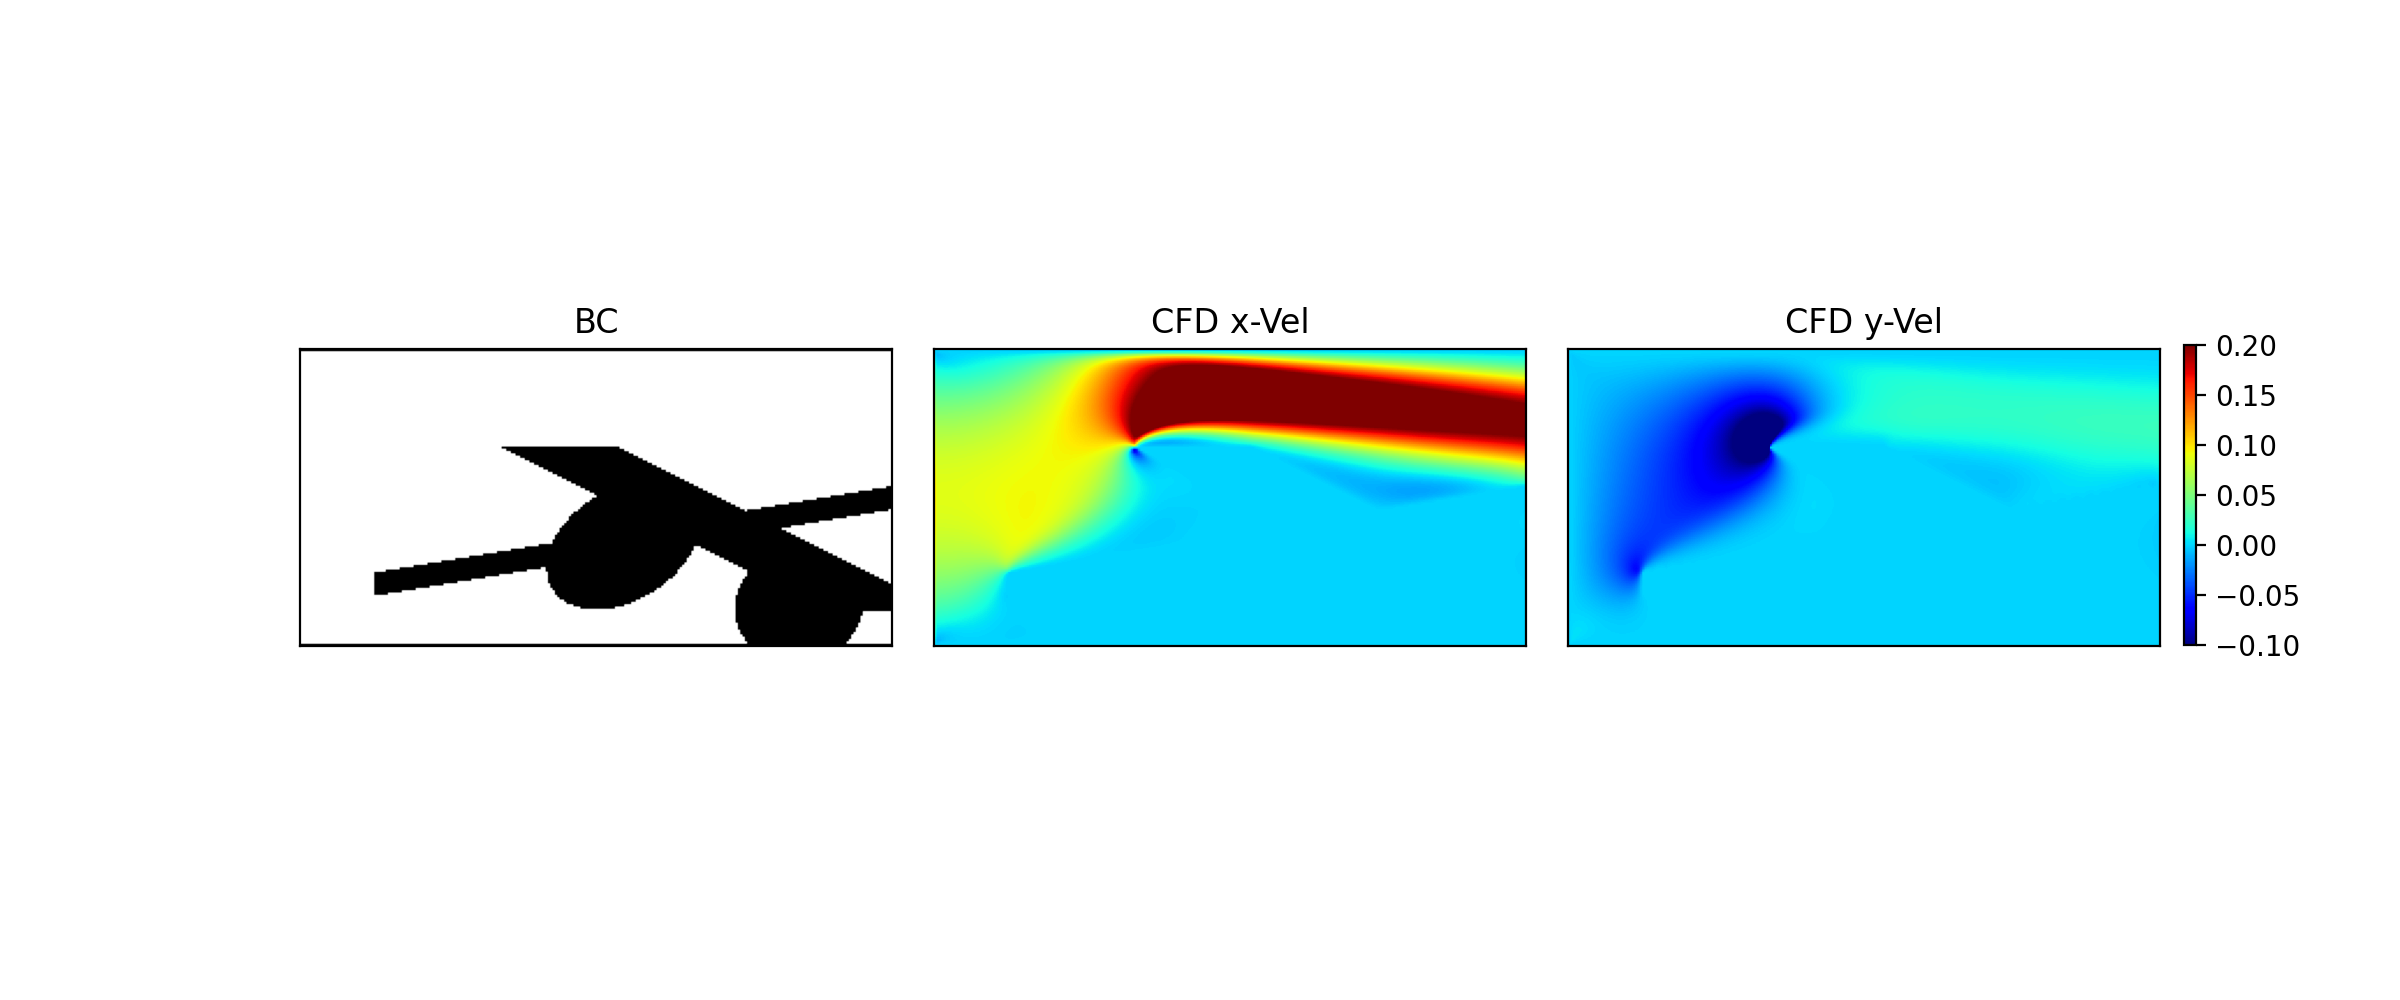
\includegraphics[height=0.16\linewidth, trim = 3.680cm 4.35cm 18.98cm 4.29cm, clip]{../../../plots/plots/train_data/montage_train_data_06.png}%

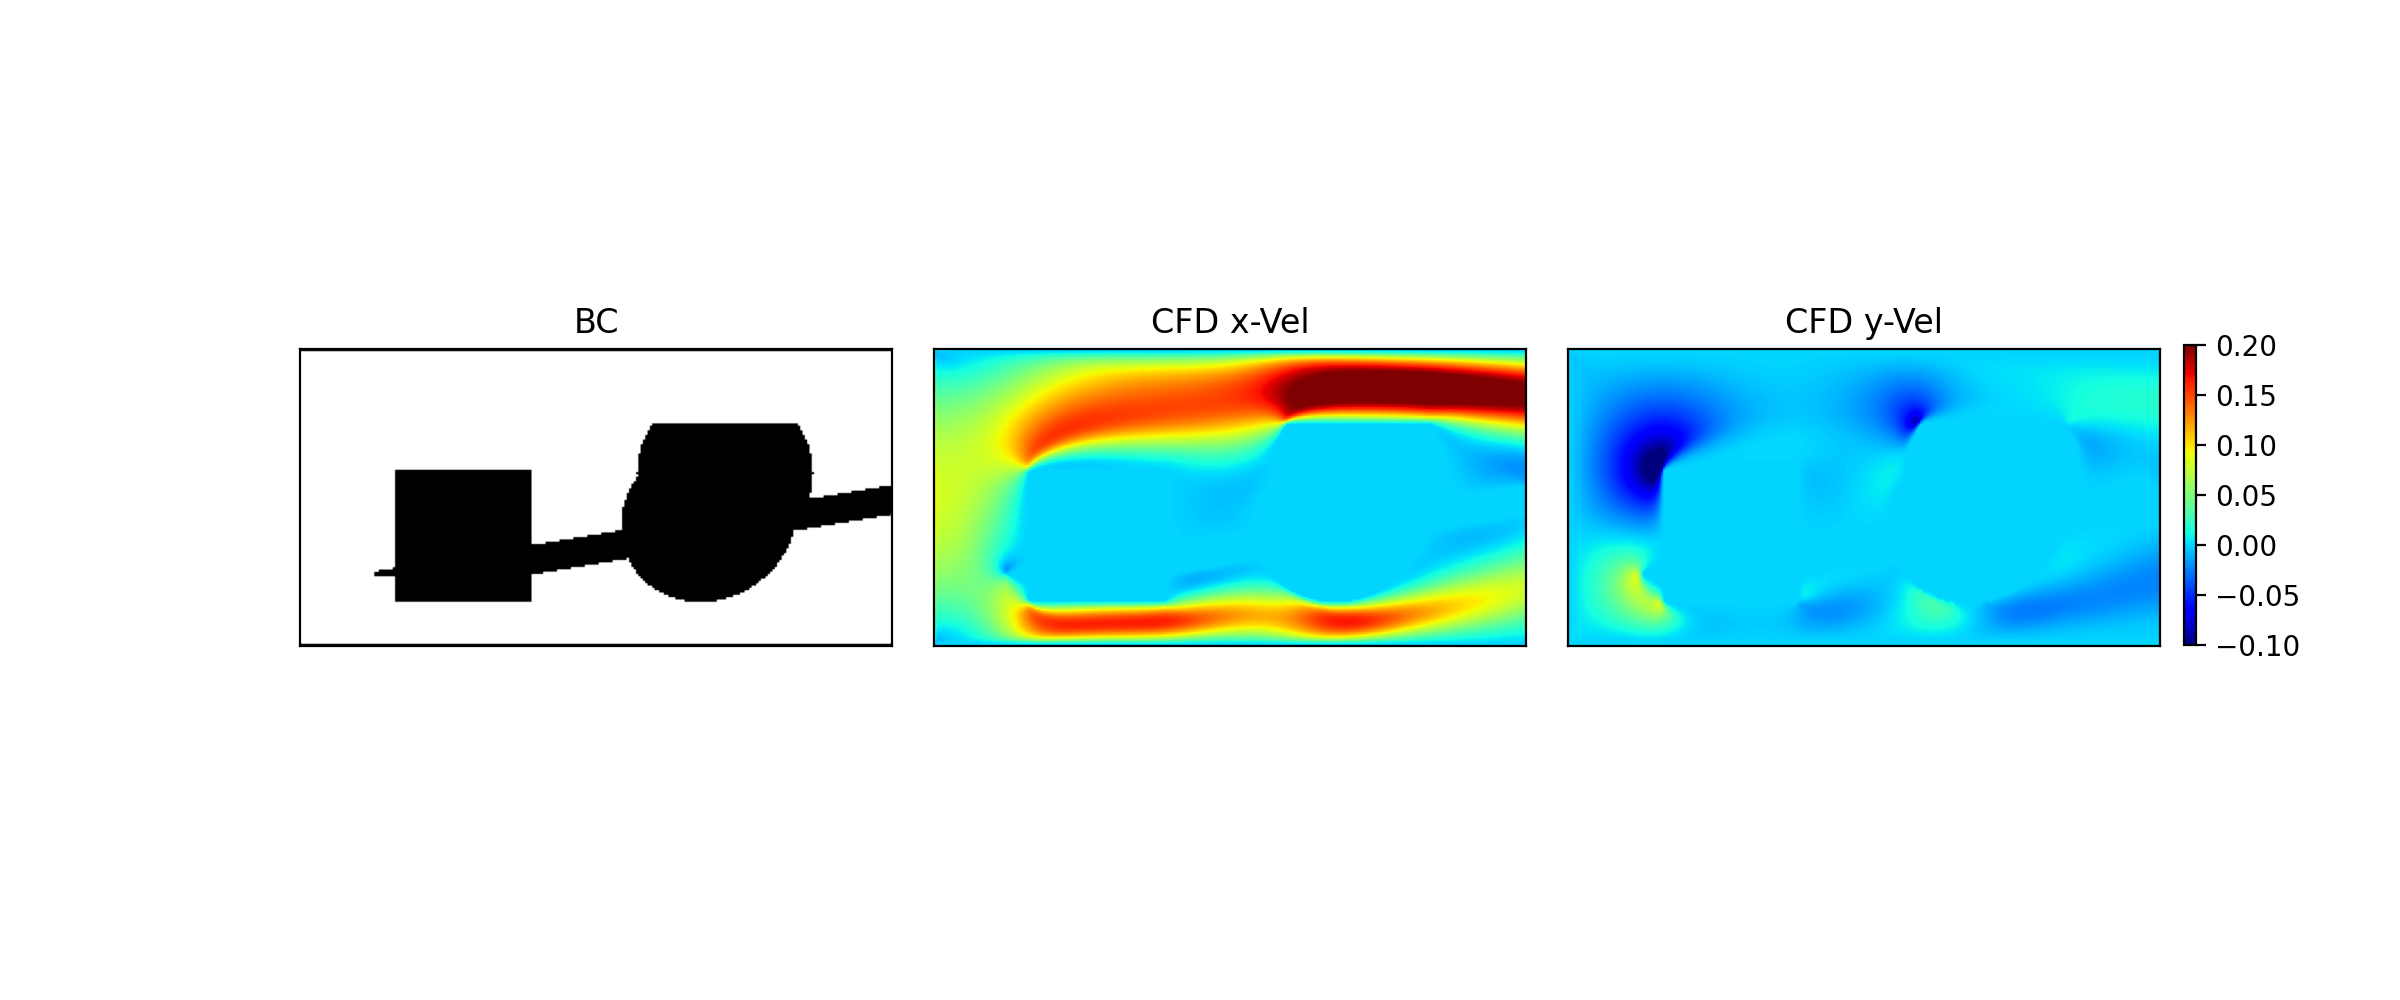
\includegraphics[height=0.16\linewidth, trim = 3.680cm 4.35cm 18.98cm 4.29cm, clip]{../../../plots/plots/train_data/montage_train_data_07.png}%      
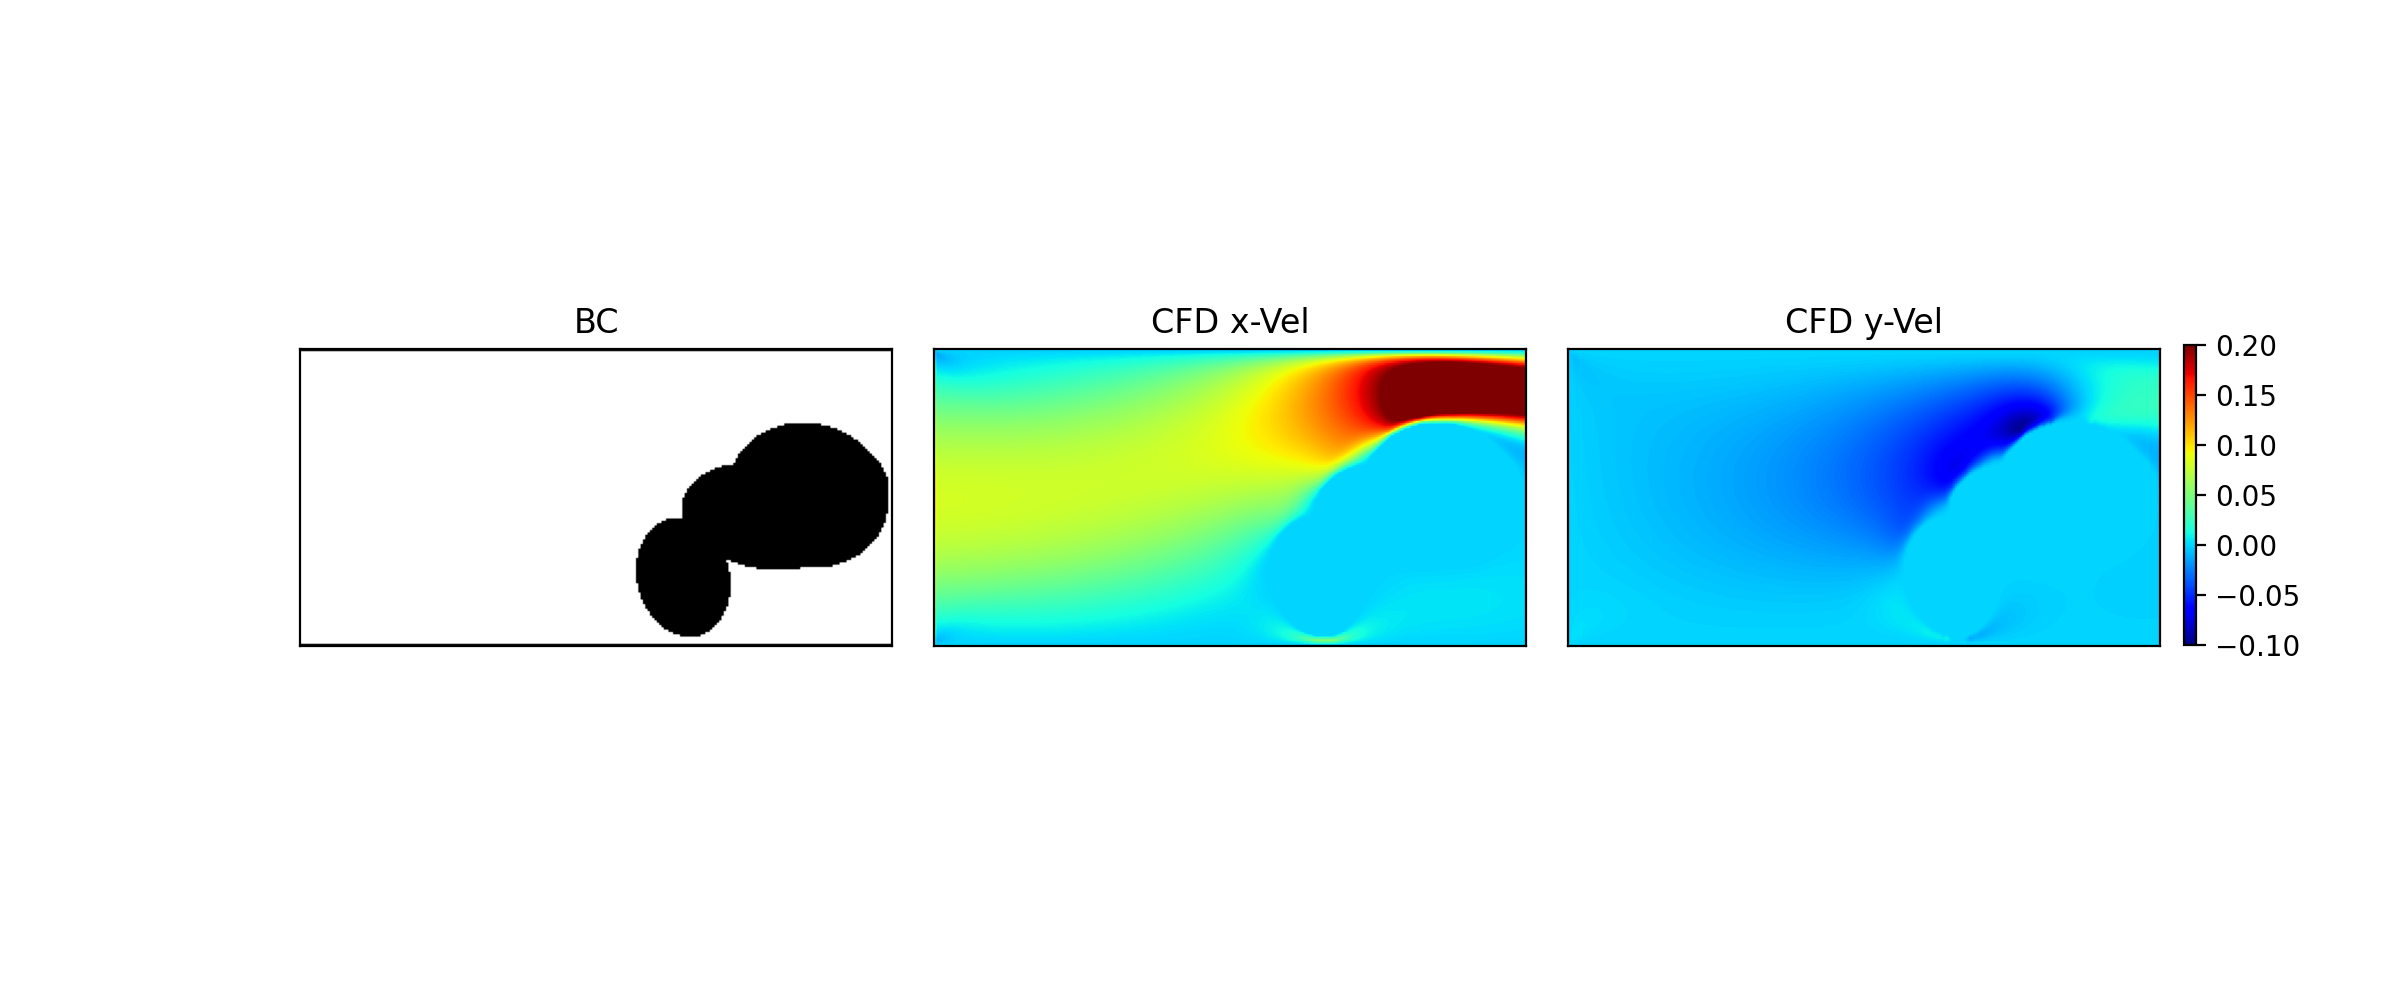
\includegraphics[height=0.16\linewidth, trim = 3.680cm 4.35cm 18.98cm 4.29cm, clip]{../../../plots/plots/train_data/montage_train_data_08.png}%
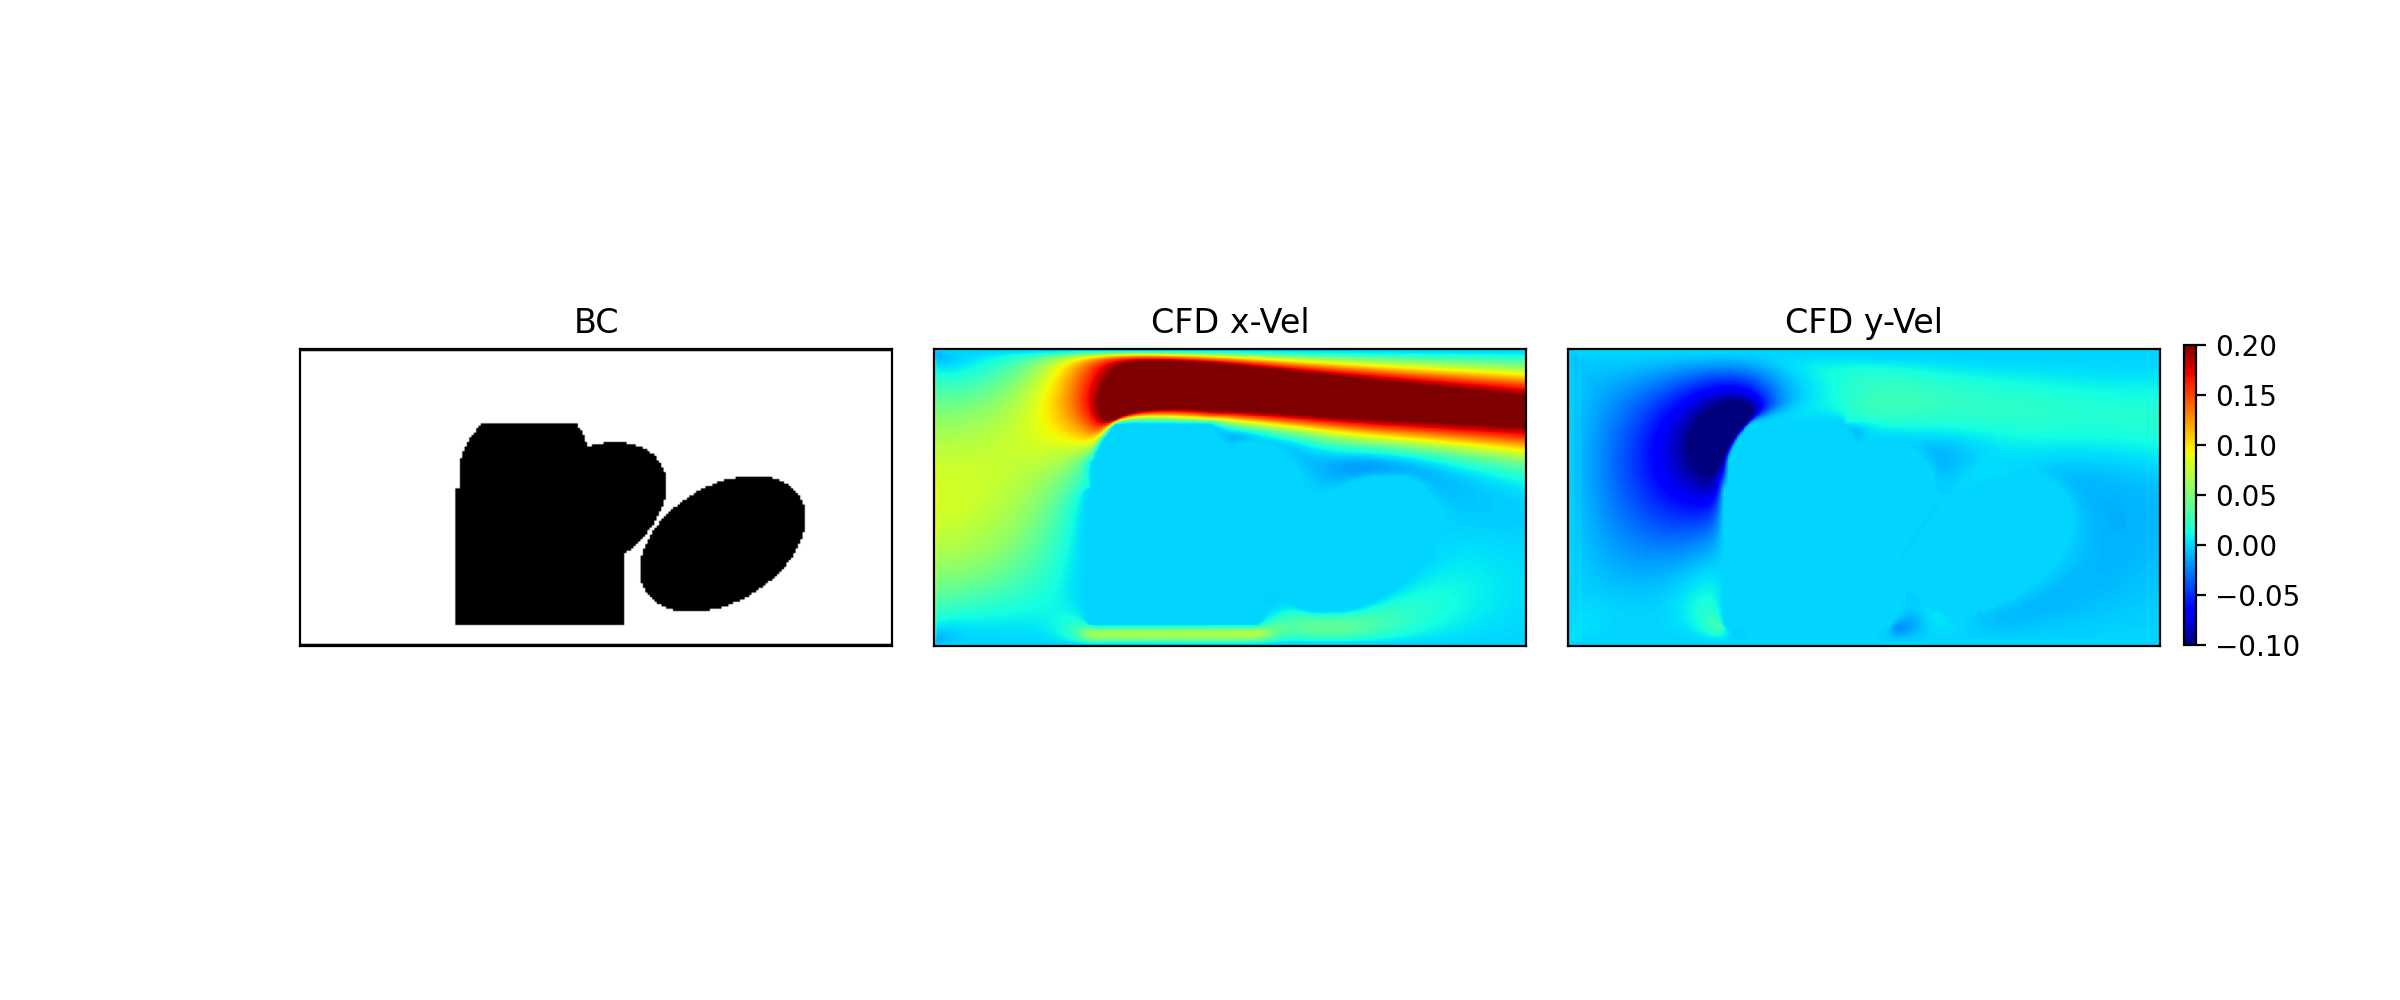
\includegraphics[height=0.16\linewidth, trim = 3.680cm 4.35cm 18.98cm 4.29cm, clip]{../../../plots/plots/train_data/montage_train_data_09.png}%

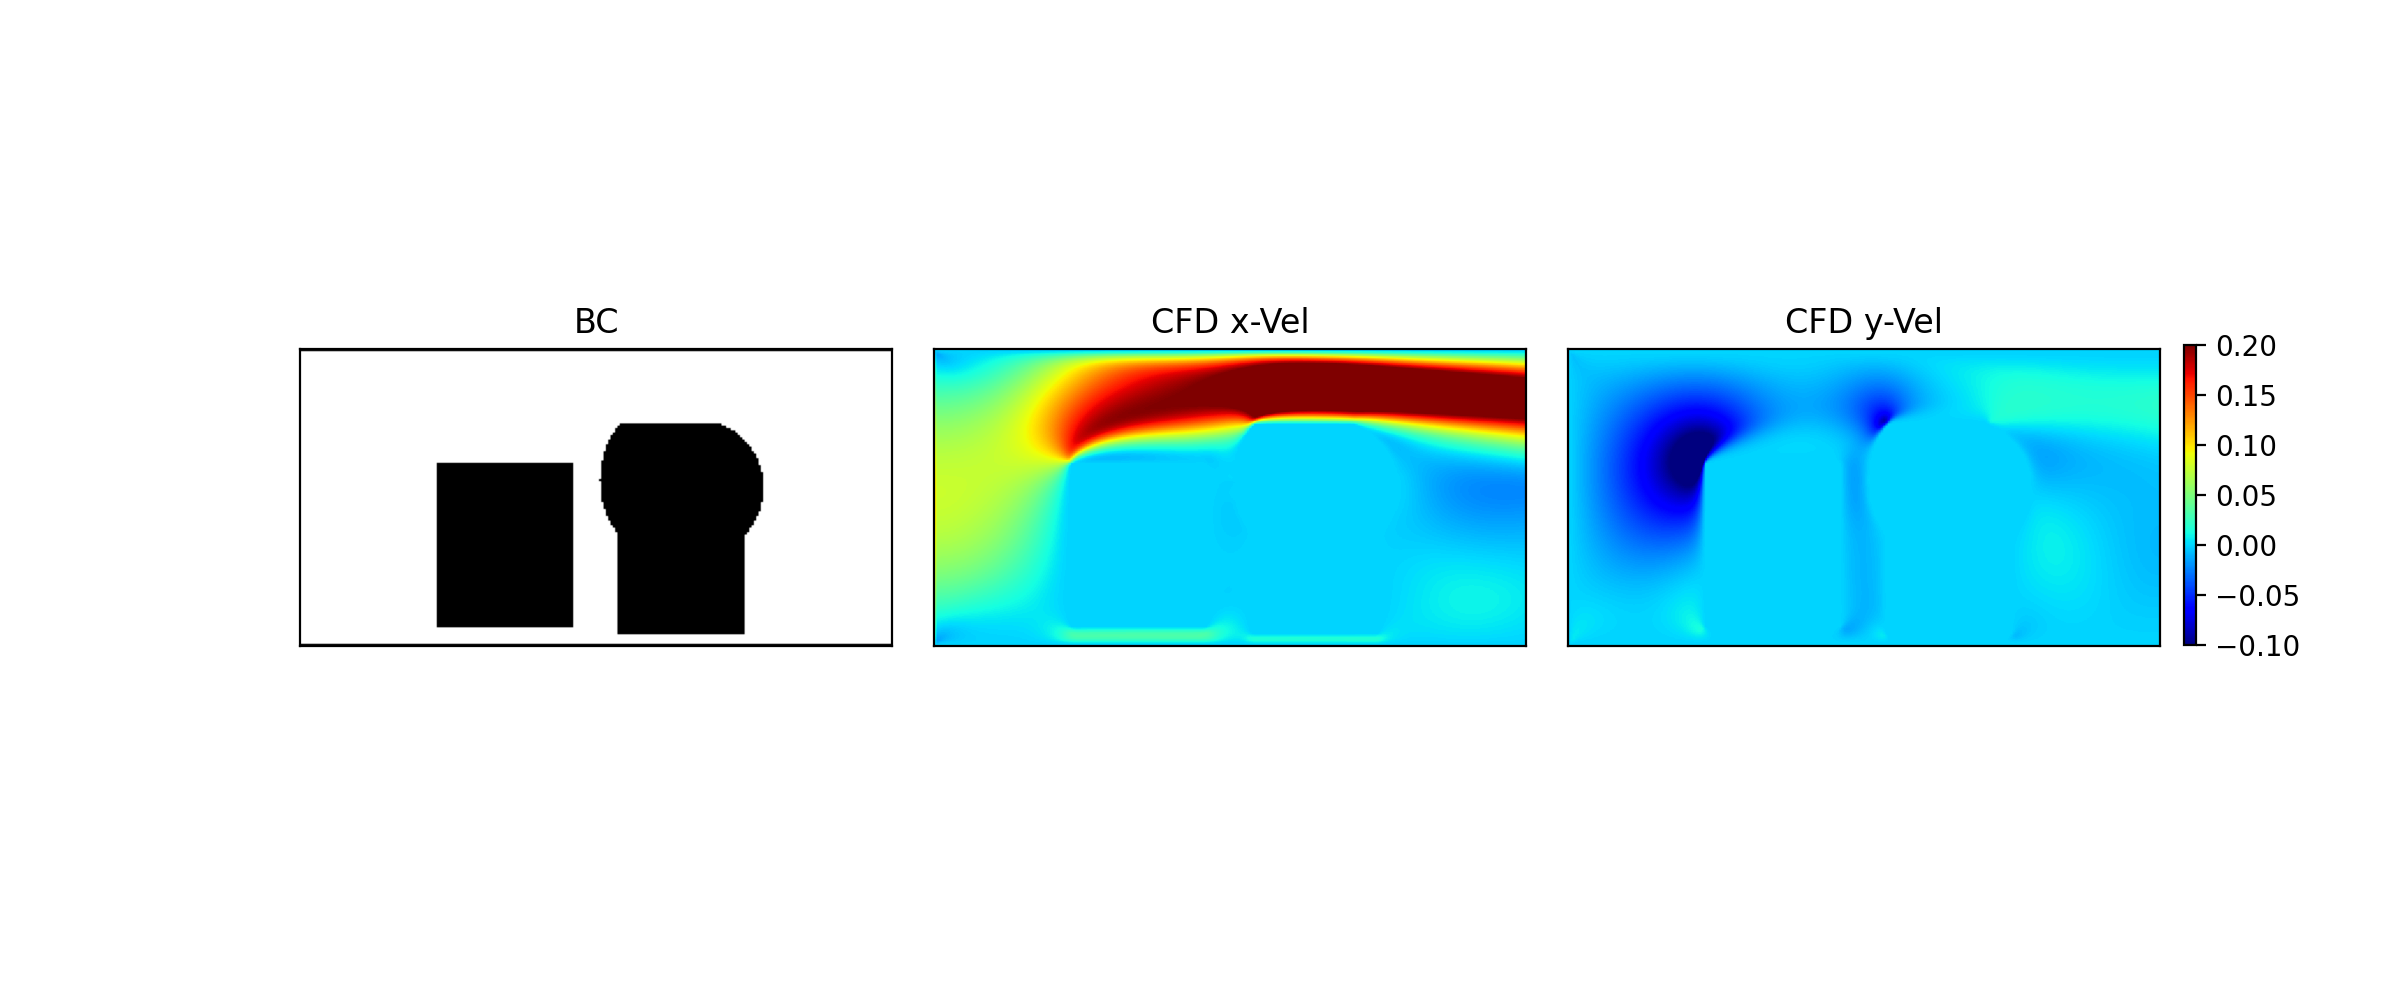
\includegraphics[height=0.16\linewidth, trim = 3.680cm 4.35cm 18.98cm 4.29cm, clip]{../../../plots/plots/train_data/montage_train_data_10.png}%      
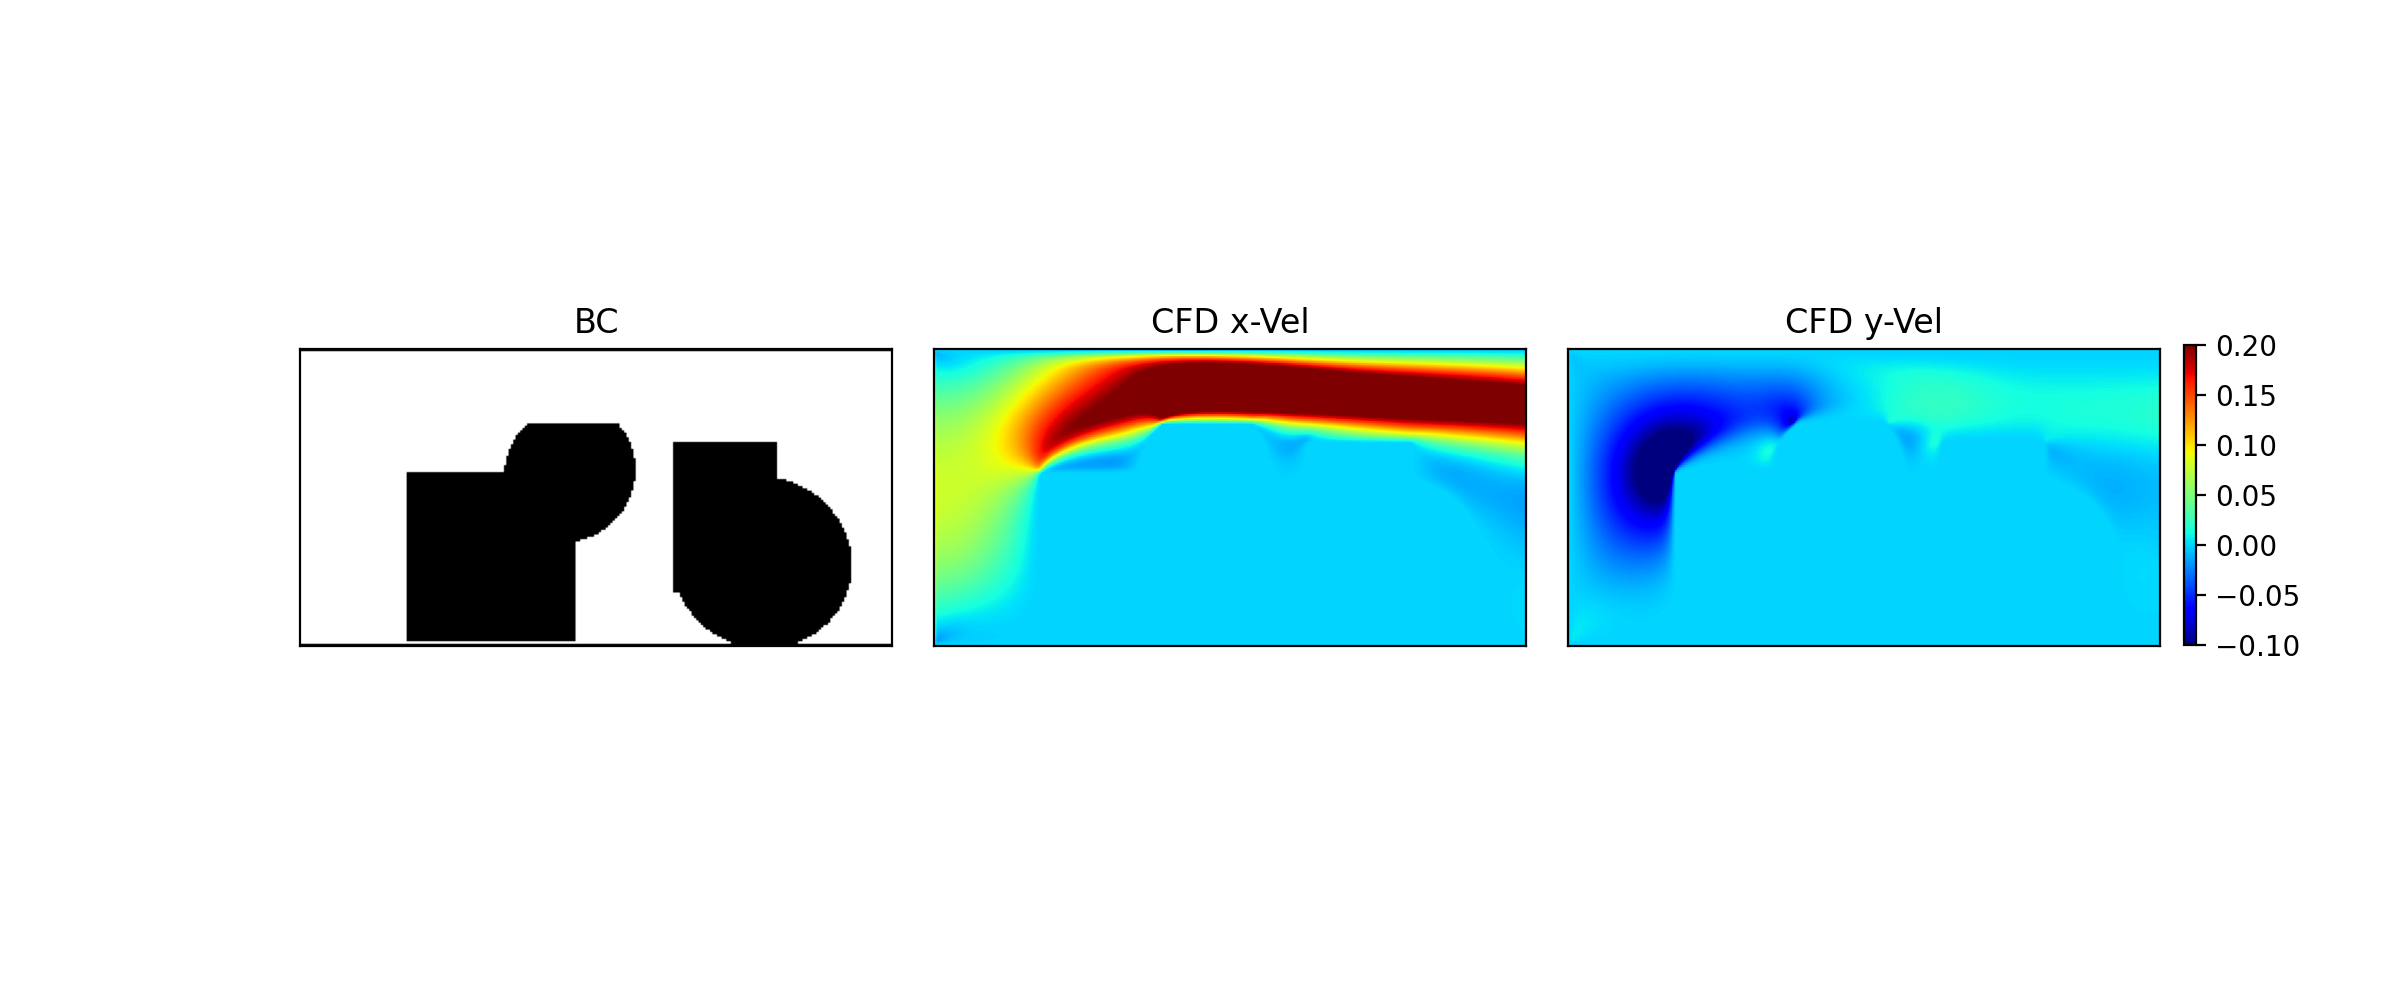
\includegraphics[height=0.16\linewidth, trim = 3.680cm 4.35cm 18.98cm 4.29cm, clip]{../../../plots/plots/train_data/montage_train_data_11.png}%
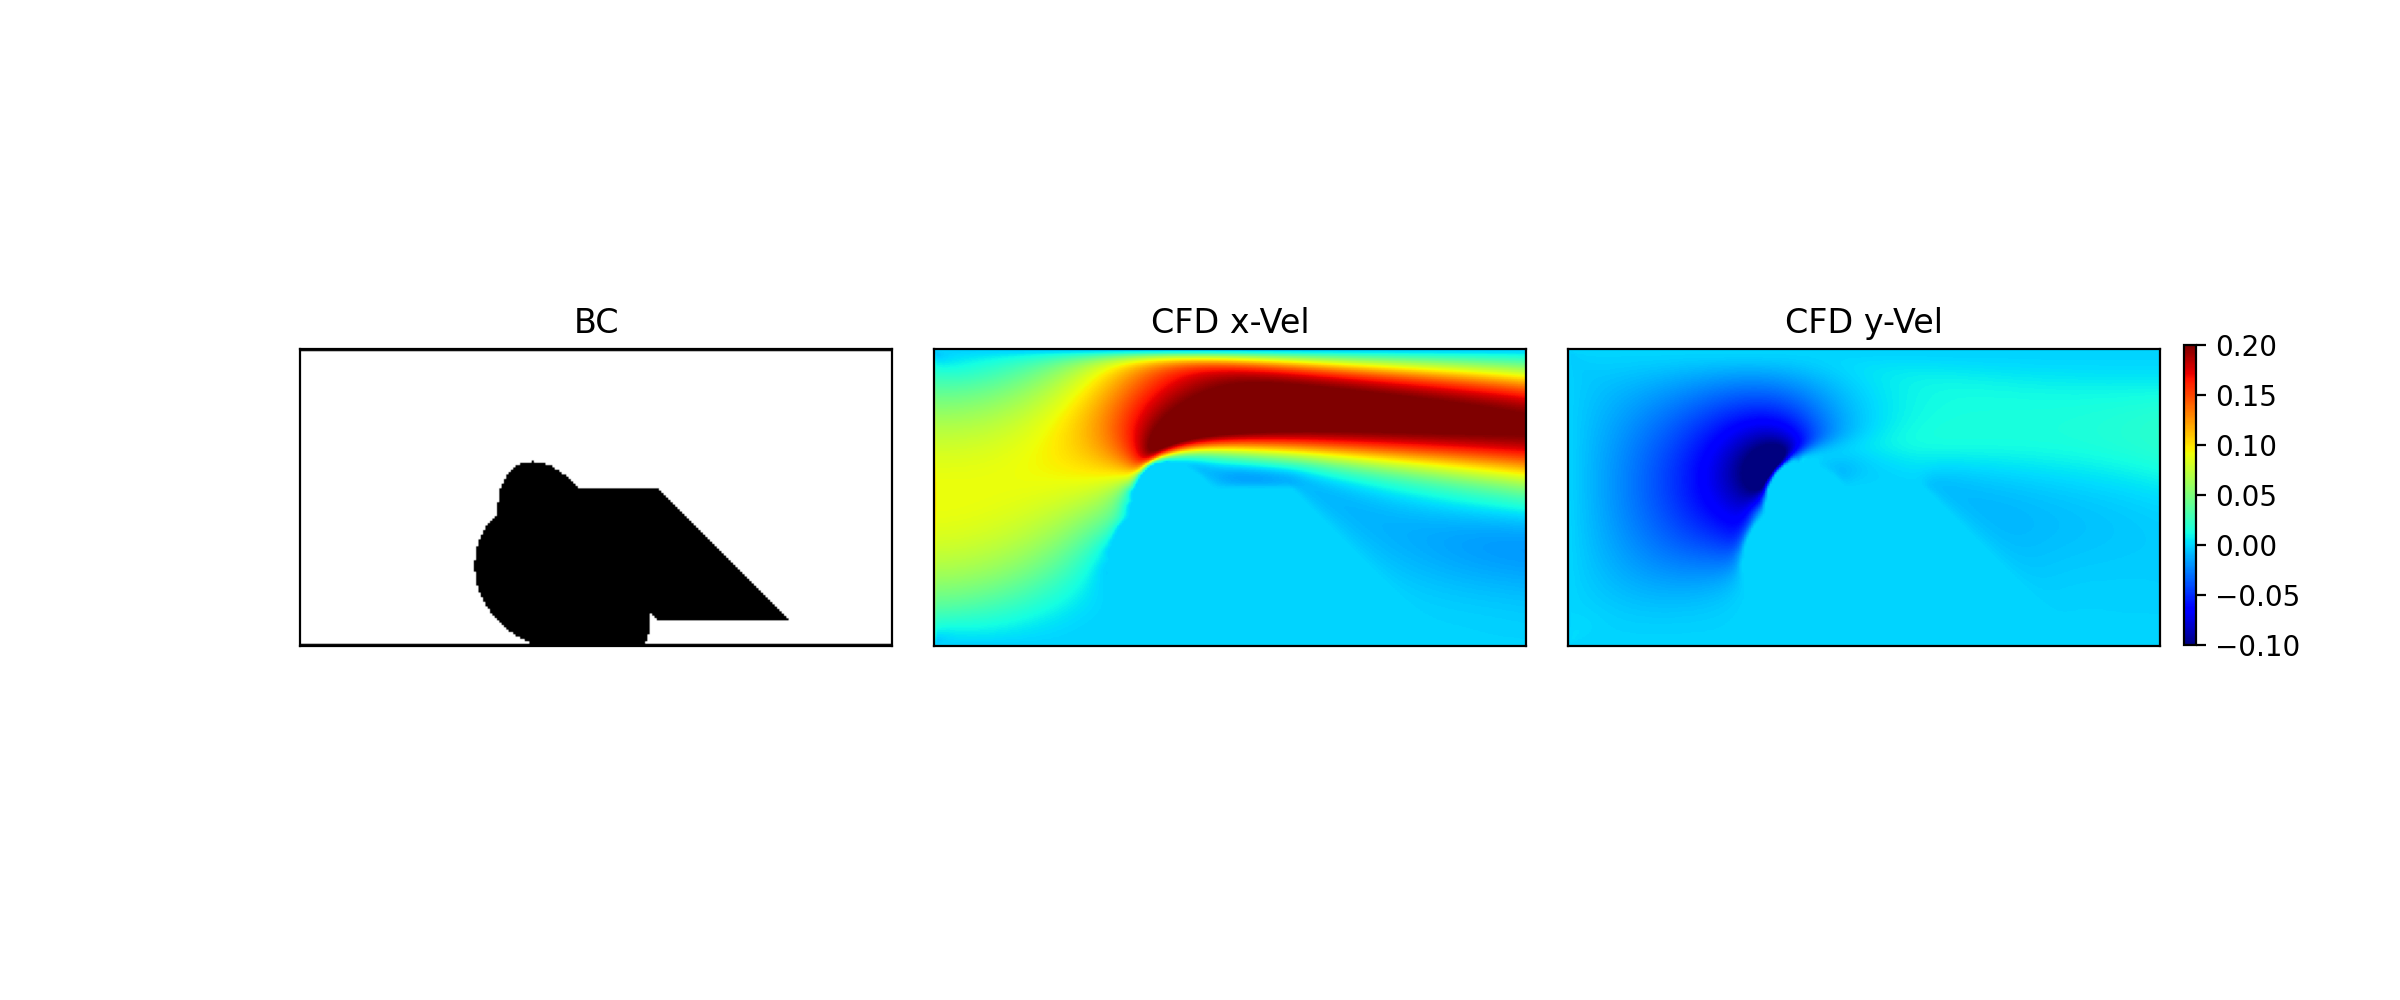
\includegraphics[height=0.16\linewidth, trim = 3.680cm 4.35cm 18.98cm 4.29cm, clip]{../../../plots/plots/train_data/montage_train_data_12.png}%
\end{figure}
\end{frame}

\begin{frame}
\frametitle{Training Data: CFD}
\begin{figure}[!htb]%

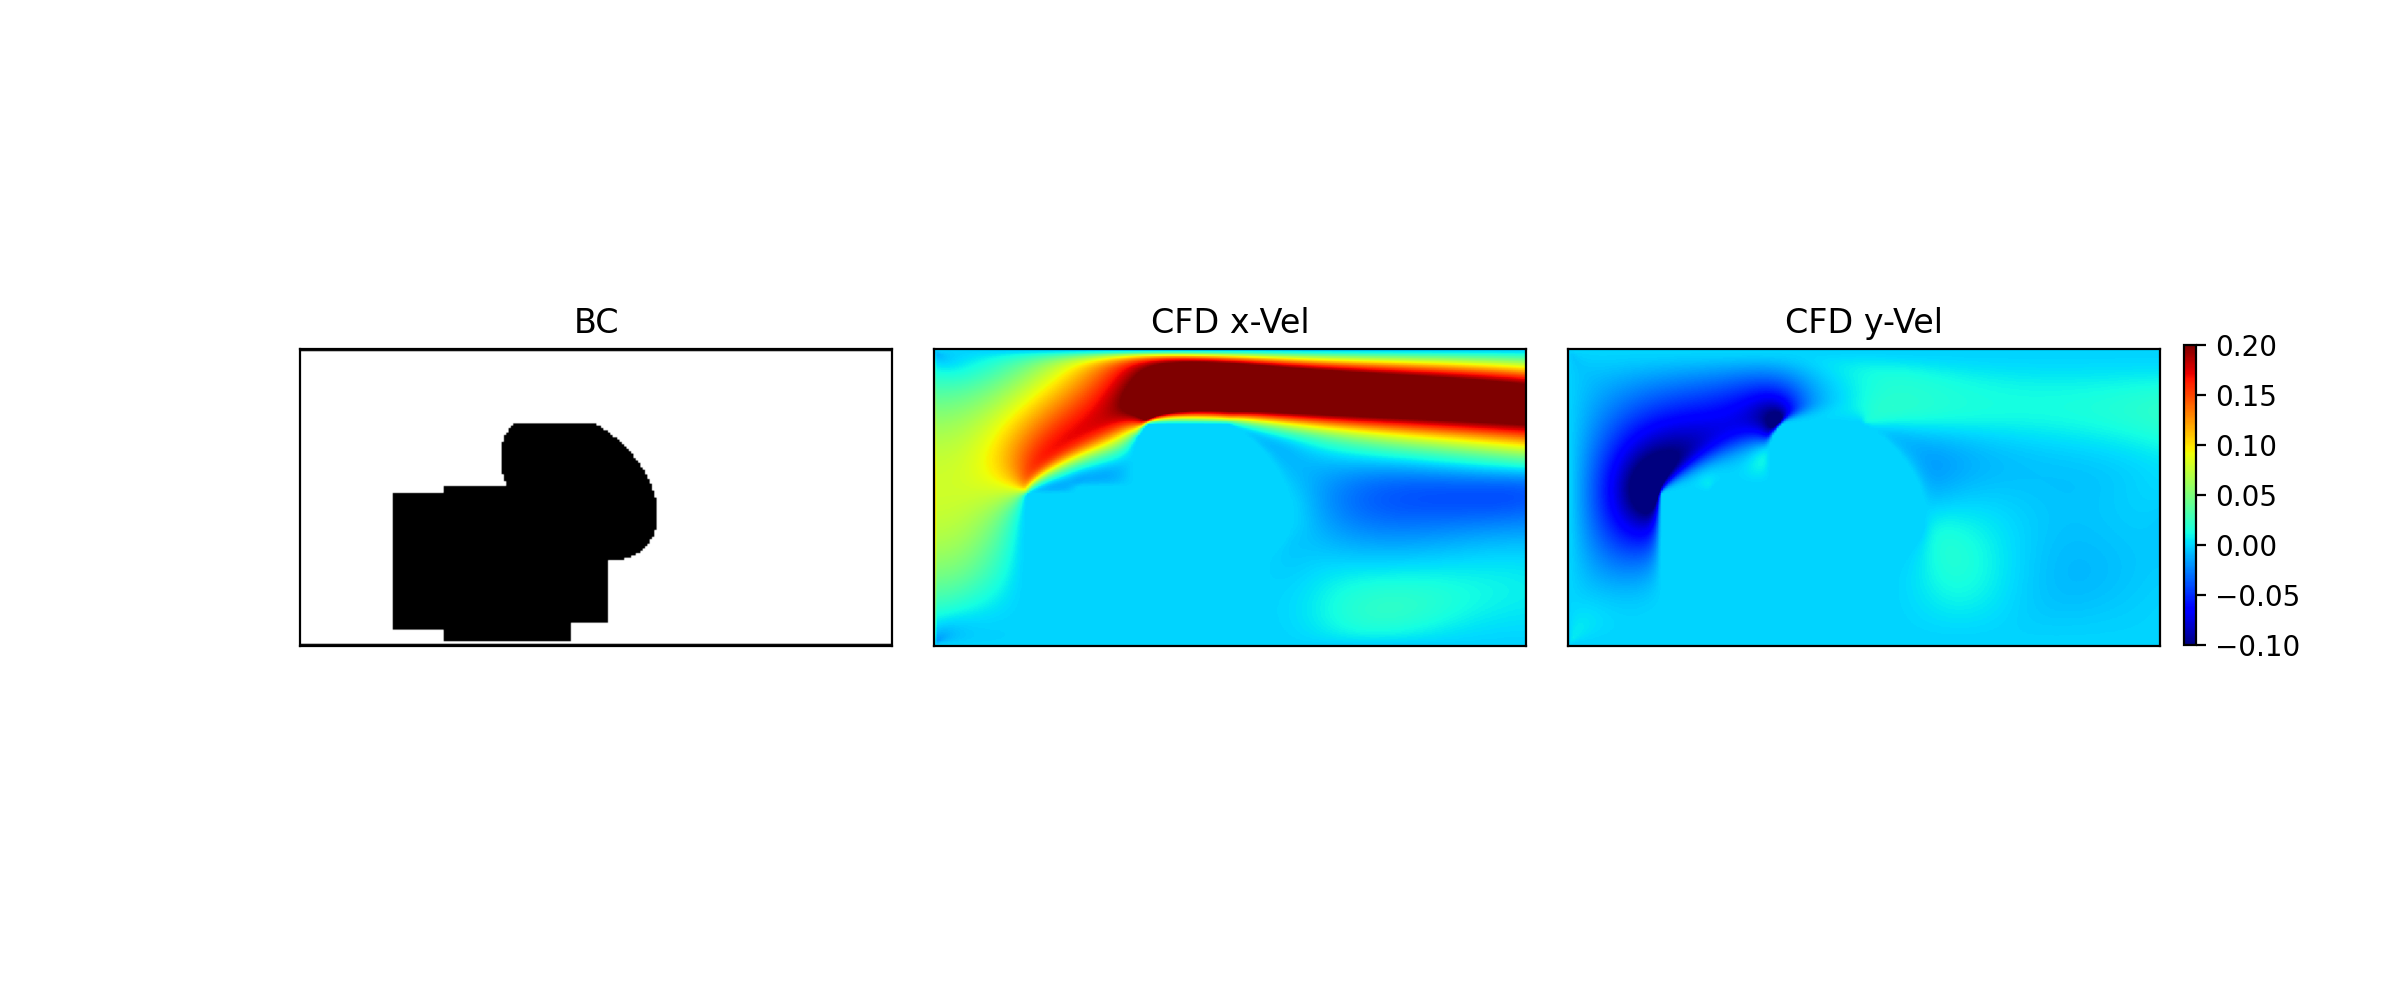
\includegraphics[height=0.20\linewidth, trim = 3.80cm 3.4cm 1.3cm 3.90cm, clip]{../../../plots/plots/train_data/montage_train_data_16.png}%
        
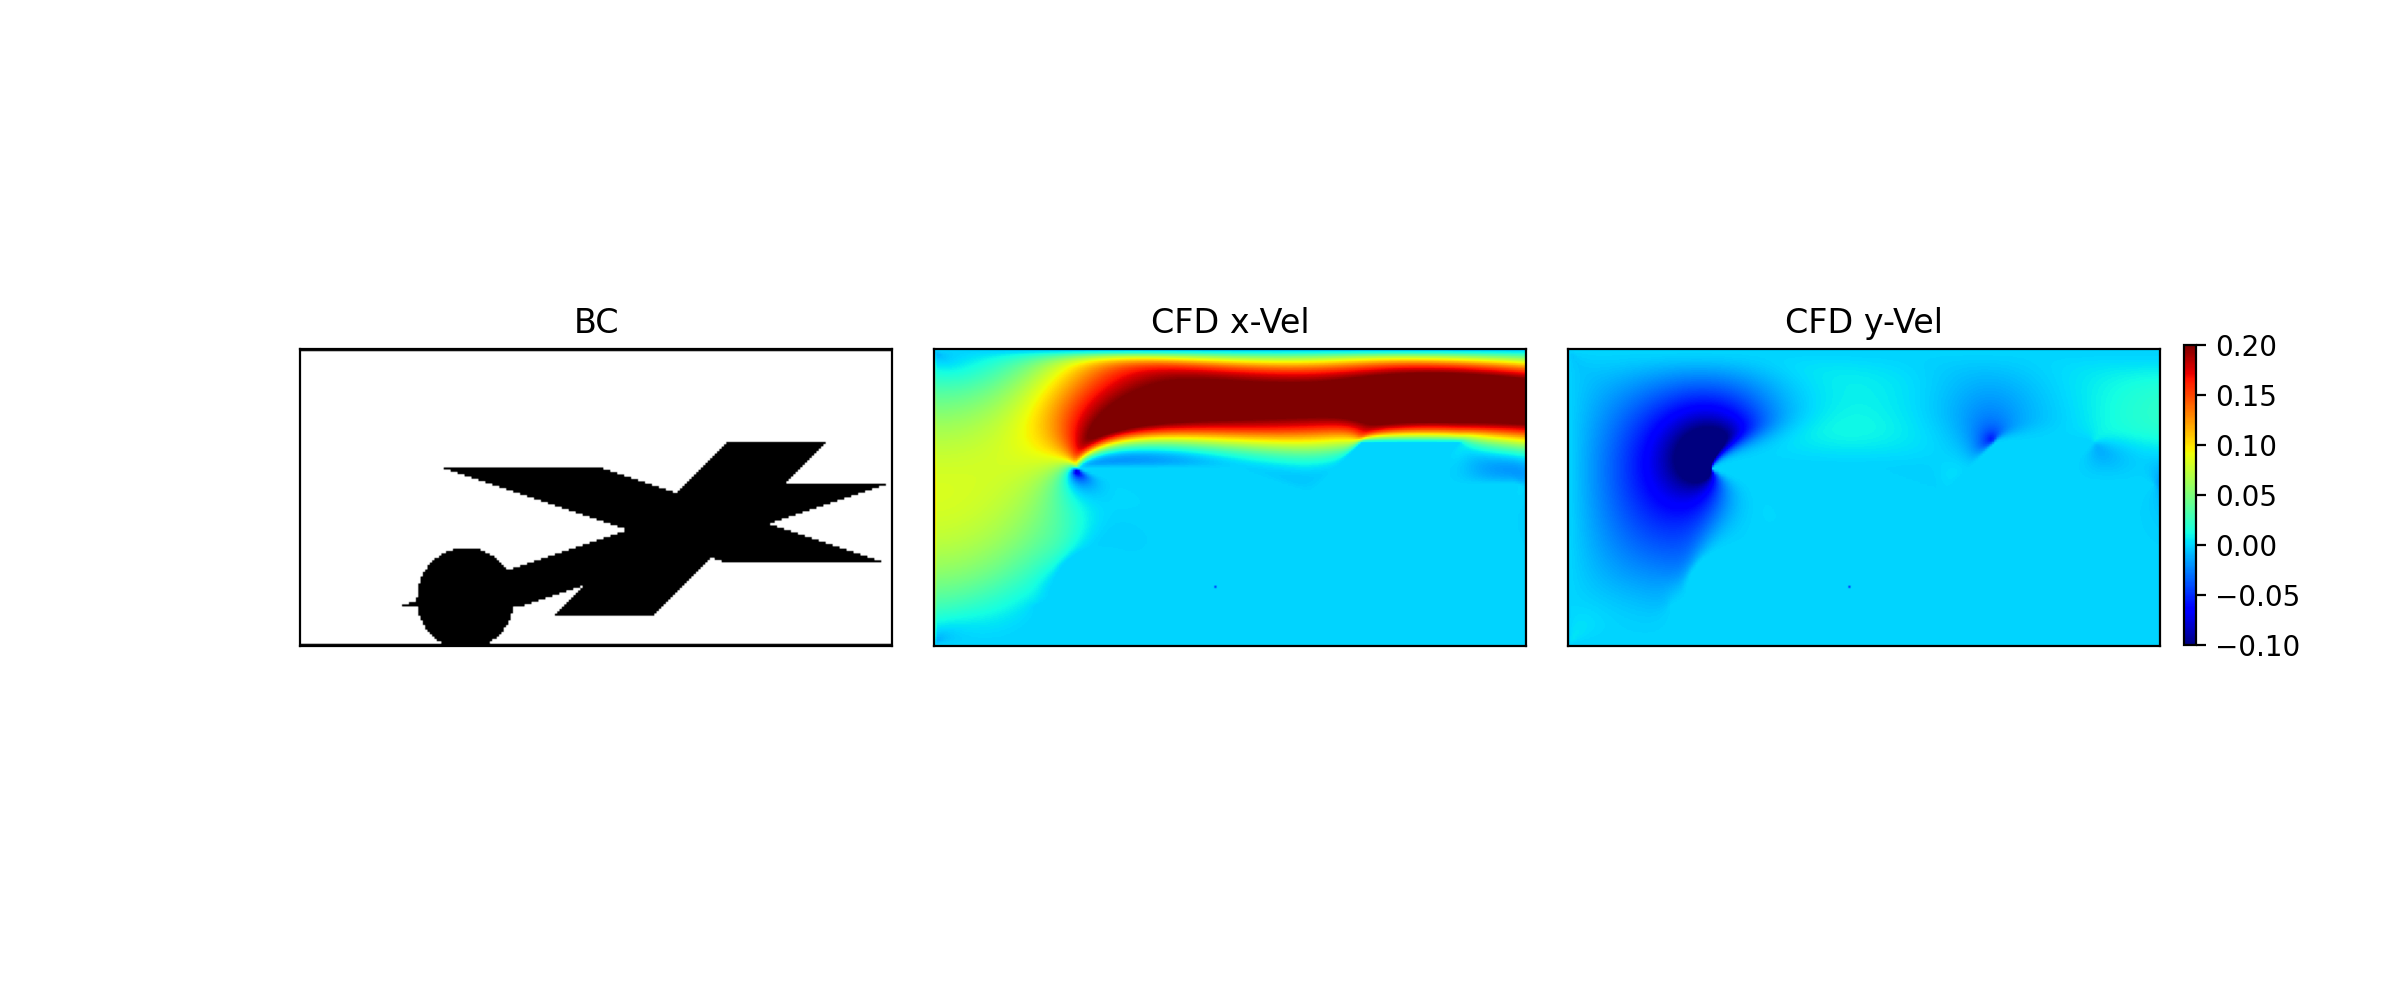
\includegraphics[height=0.20\linewidth, trim = 3.80cm 3.4cm 1.3cm 3.90cm, clip]{../../../plots/plots/train_data/montage_train_data_17.png}%

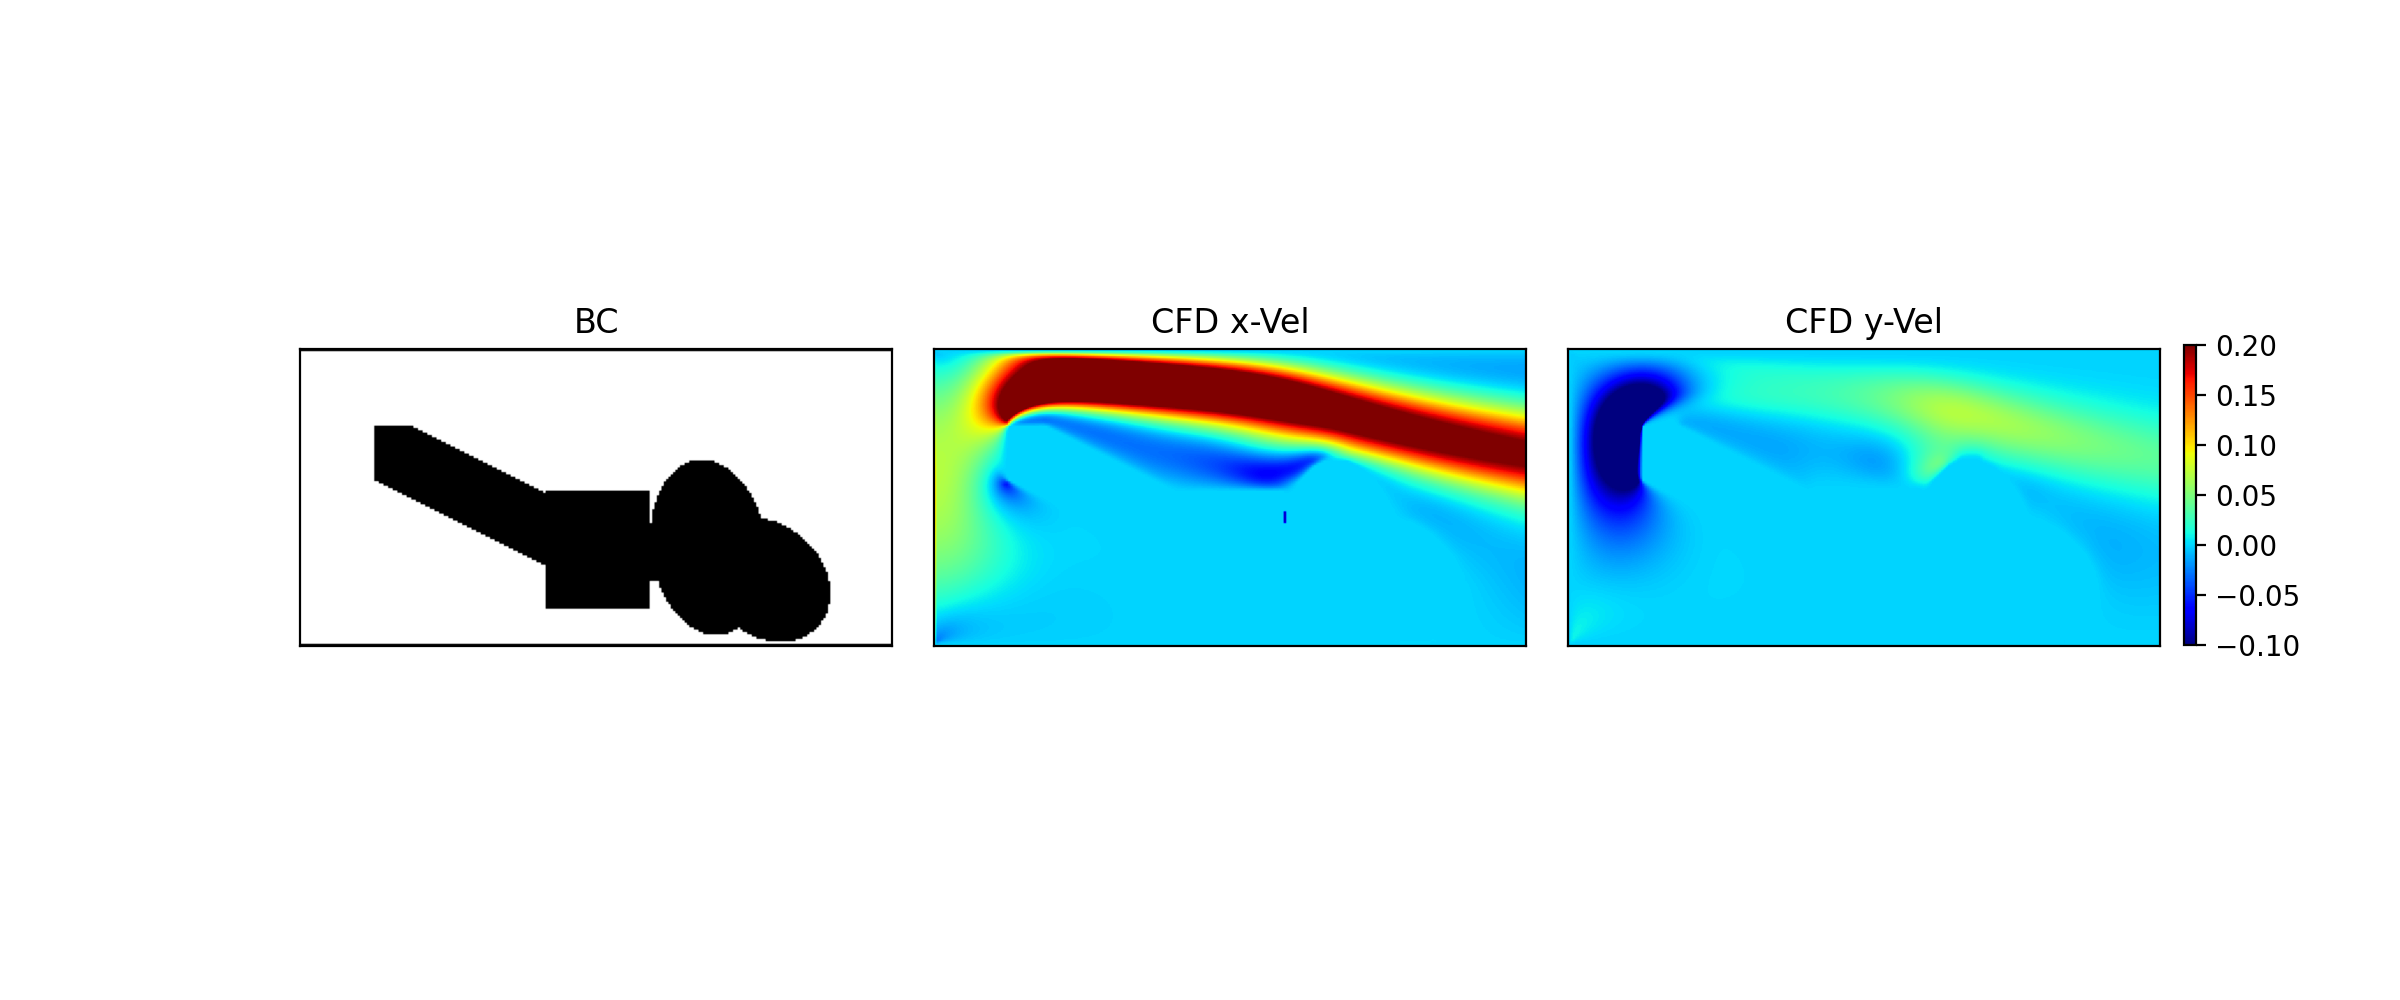
\includegraphics[height=0.20\linewidth, trim = 3.80cm 3.4cm 1.3cm 3.90cm, clip]{../../../plots/plots/train_data/montage_train_data_18.png}%
\vspace{-0.20cm}
\caption{BCs, CFD Results}
\end{figure}
\end{frame}


\begin{frame}
\frametitle{Training Data}
\begin{figure}[!htb]%
\caption{This slide contains a movie}
\end{figure}
\end{frame} 


\section{DL Approach} % A subsection can be created just before a set of slides with a common theme to further break down your presentation into chunks
\begin{frame}
\frametitle{DL Approach Overview}
\begin{itemize}
\item Training Data ~\parencite{hennighTrain}
\item Model Architectures
\item Image Loss and Metrics
\item Train Model
\item Prediction on Unseen Data
\end{itemize}
\end{frame}

\begin{frame}
\frametitle{Training Data}
\begin{itemize}
\item How complex is the problem you are trying to solve? 
\bigskip
Is training data representative from the problem we are trying to solve?
\bigskip
\item Generate 50,000 $\Longrightarrow$ 10,000 $\Longrightarrow$ 5,000 records
\bigskip
\item Training and test records drawn from same distribution (idd)
\end{itemize}
\end{frame}

\begin{frame}
\frametitle{Architectures: CNNs ~\parencite{guo2016convolutional}}
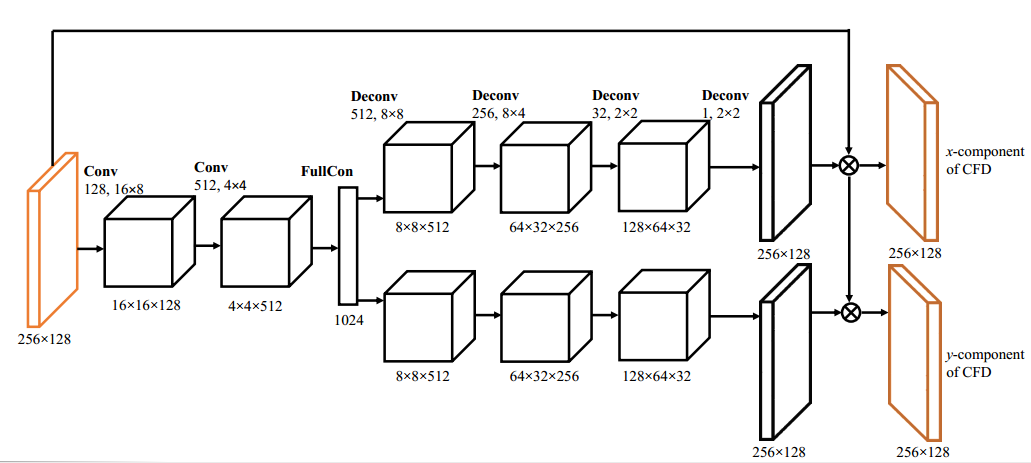
\includegraphics[width=12cm,trim = 0cm 0.2cm 0cm 0cm, clip]{img/guo_convNets.png}
\end{frame}

\begin{frame}
\frametitle{Architectures: ResNet  ~\parencite{he2016deep}}
\begin{figure}[h]
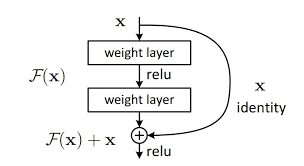
\includegraphics[width=12cm,trim = 0cm 0.0cm 0cm 0cm, clip]{img/resnet_idea.png}
\end{figure}
\end{frame}

\begin{frame}
\frametitle{Architectures: U-Net~\parencite{ronneberger2015u}}
\begin{figure}[h]
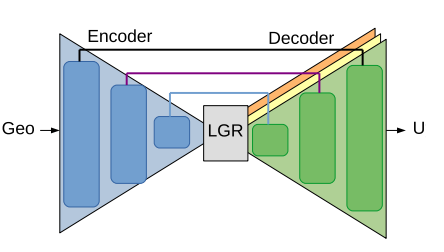
\includegraphics[width=12cm, trim = 0cm 0.0cm 0cm 0cm, clip]{img/UNet-1Encoder.png}
\caption{~\parencite{ribeiro2020deepcfd}}
\end{figure}
\end{frame}


\begin{frame}
\frametitle{Our Architecture: CNN + U-Net + ResNet}
\begin{figure}[h]
\hspace{-1cm}
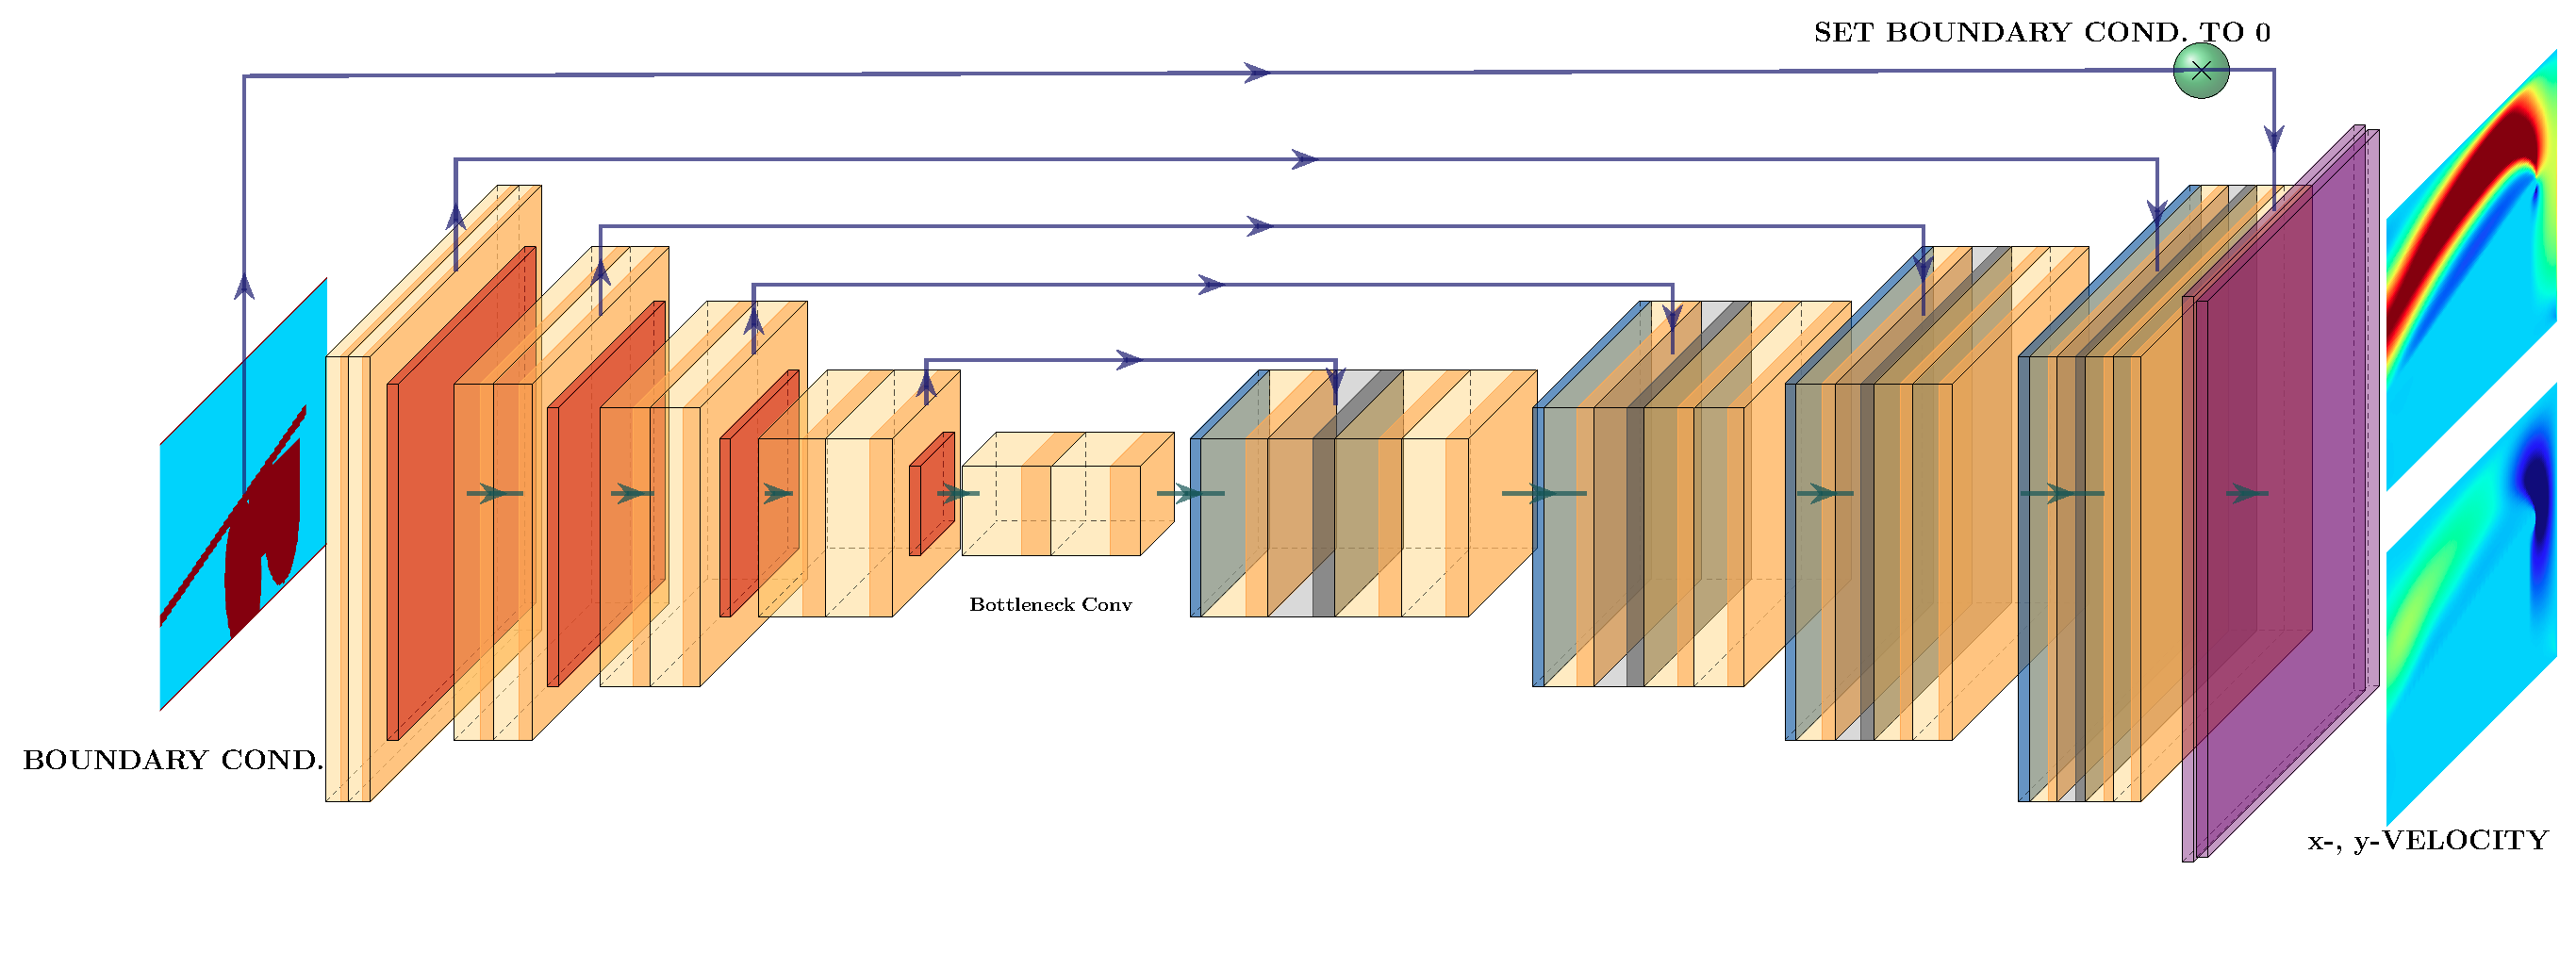
\includegraphics[width=12.5cm]{../../../plots/Unet_architecture.png}
\end{figure}
\end{frame}

\begin{frame}
\frametitle{Test Data \Smiley[1.5]}
\vspace{-0.40cm}
\begin{figure}[!htb]%
    \hspace{-0.55cm}
    \begin{minipage}{0.41\textwidth}%
       \center{
       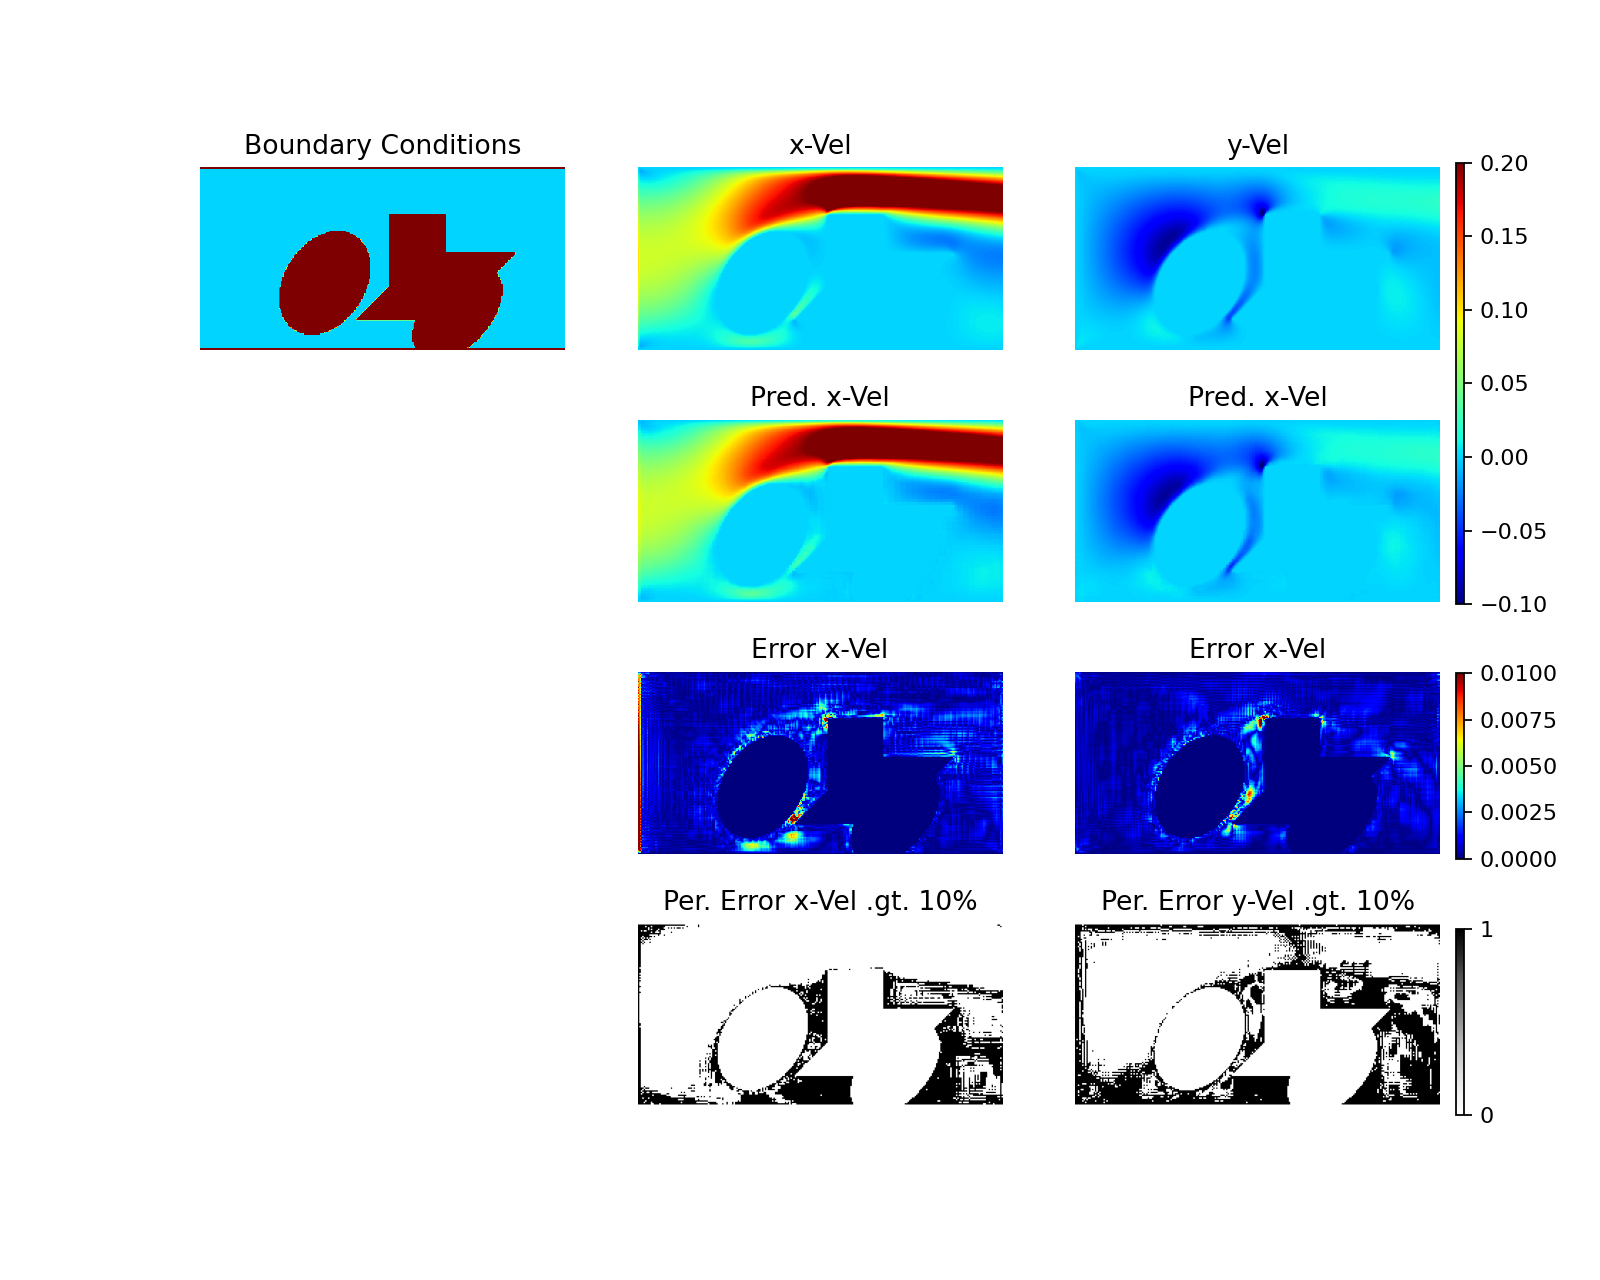
\includegraphics[width=0.5\linewidth, trim = 3.65cm 17.94cm 19.08cm 2.1cm, clip]{../../../plots/plots/test_data/montage_test_pred_0.1_30.png}%%%
       }
       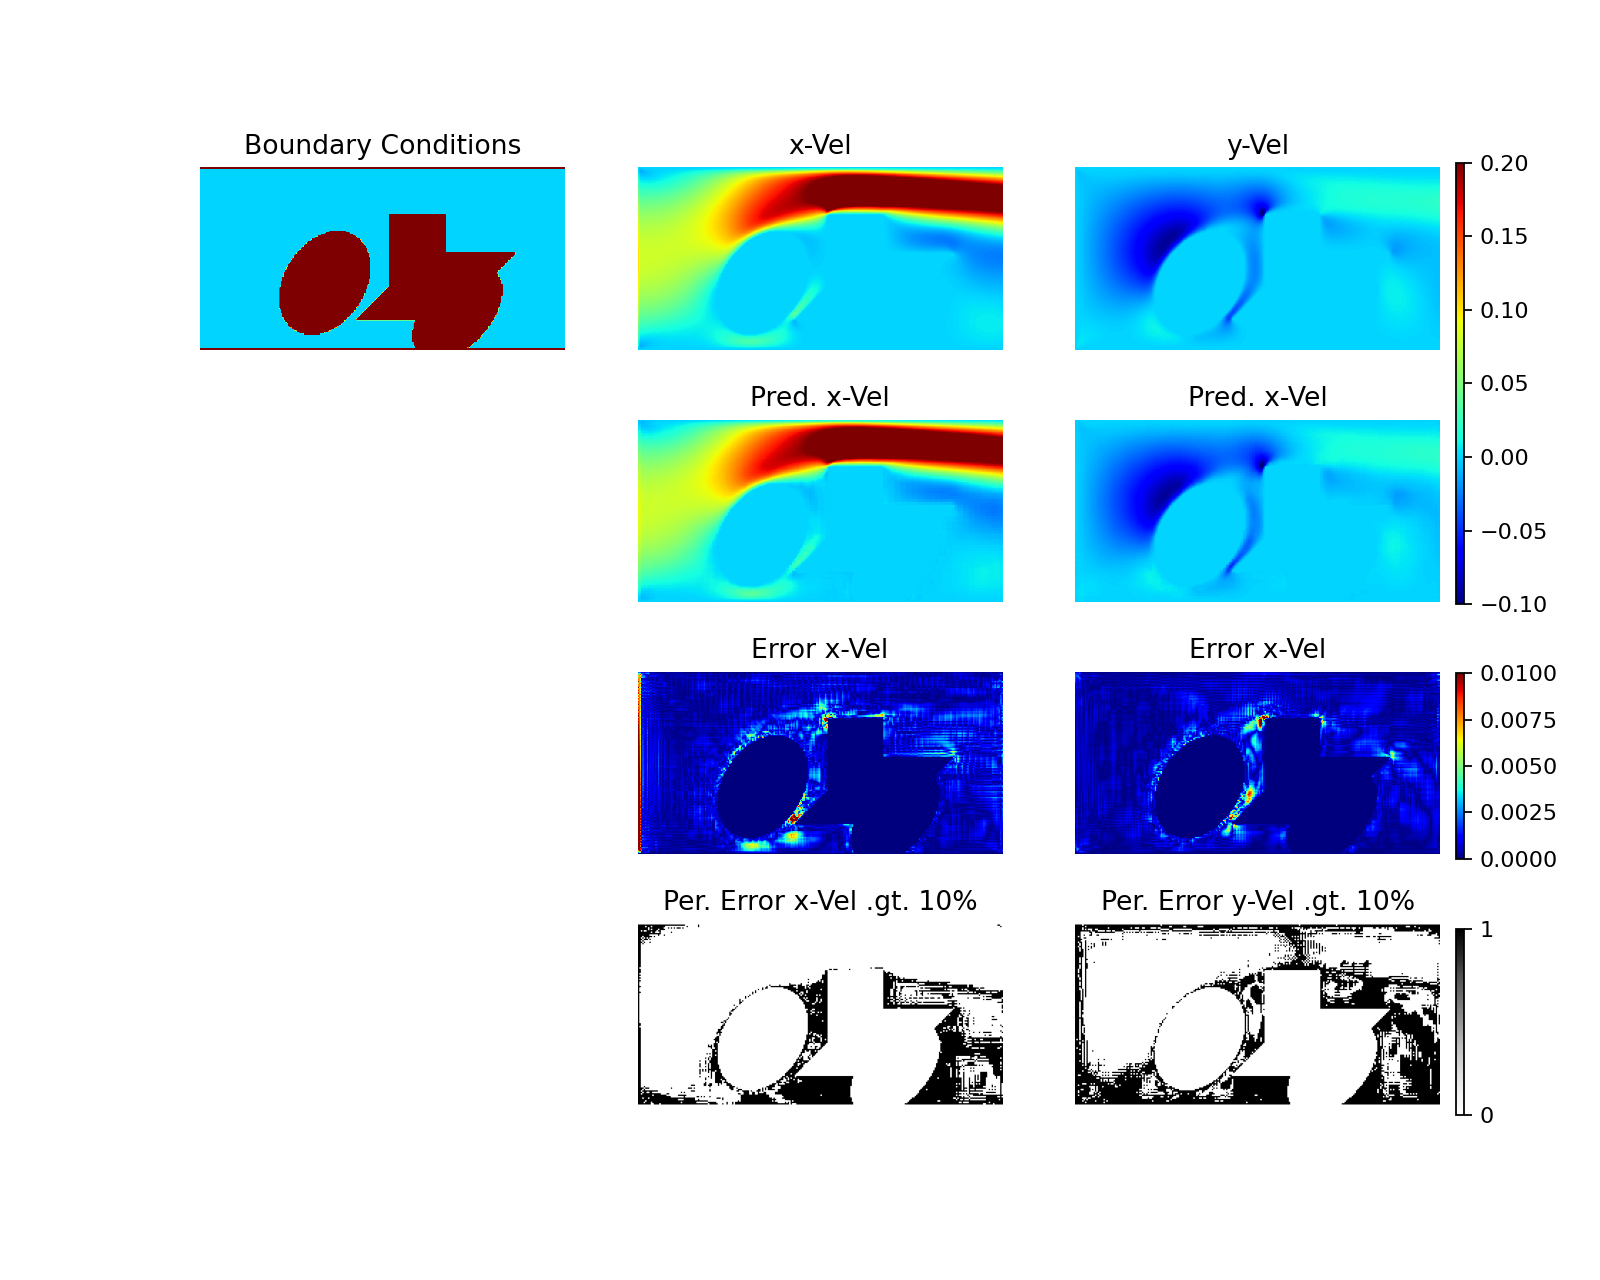
\includegraphics[width=1.0\linewidth, trim = 11.5cm 3cm 3cm 2.1cm, clip]{../../../plots/plots/test_data/montage_test_pred_0.1_30.png}%%%
    \end{minipage}%
    %
    \hspace{0.25cm}
    \begin{minipage}{0.41\textwidth}%
        \center{
        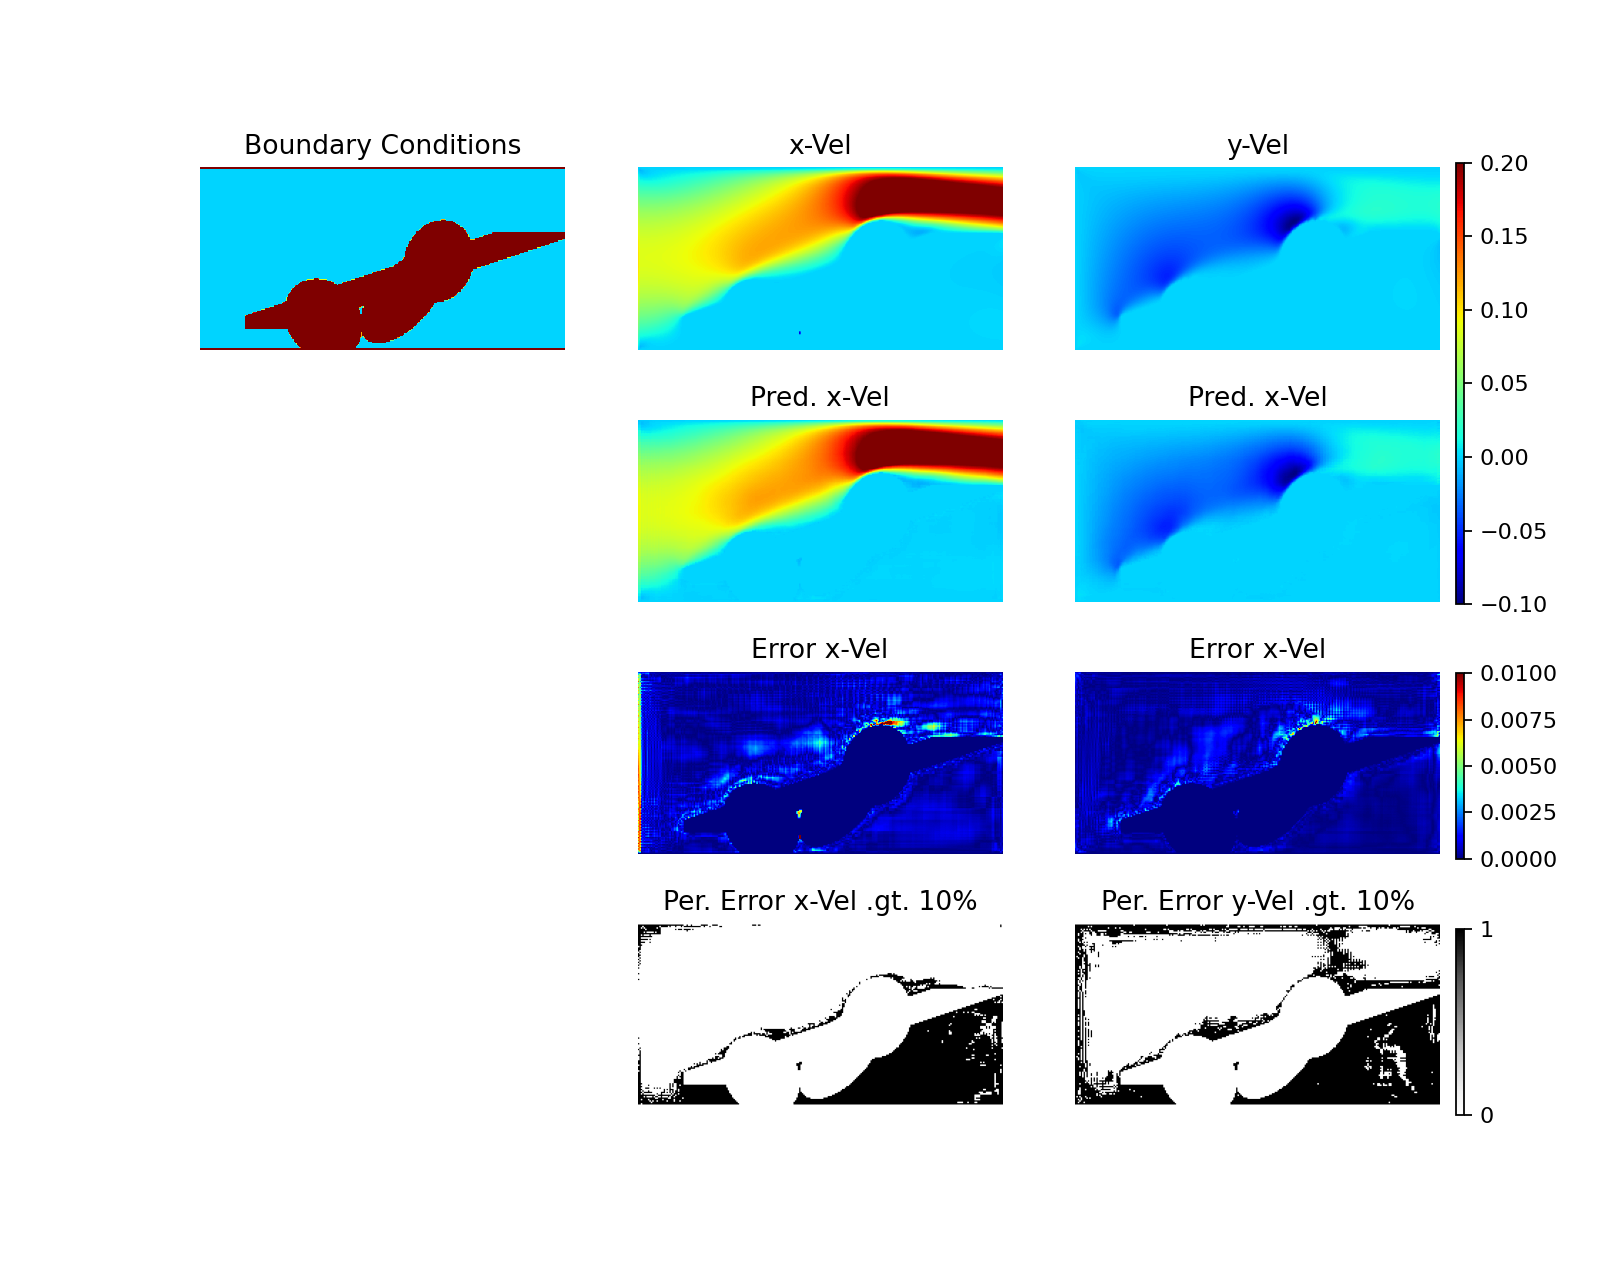
\includegraphics[width=0.5\linewidth, trim = 3.65cm 17.94cm 19.08cm 2.1cm, clip]{../../../plots/plots/test_data/montage_test_pred_0.1_81.png}%%
        }
        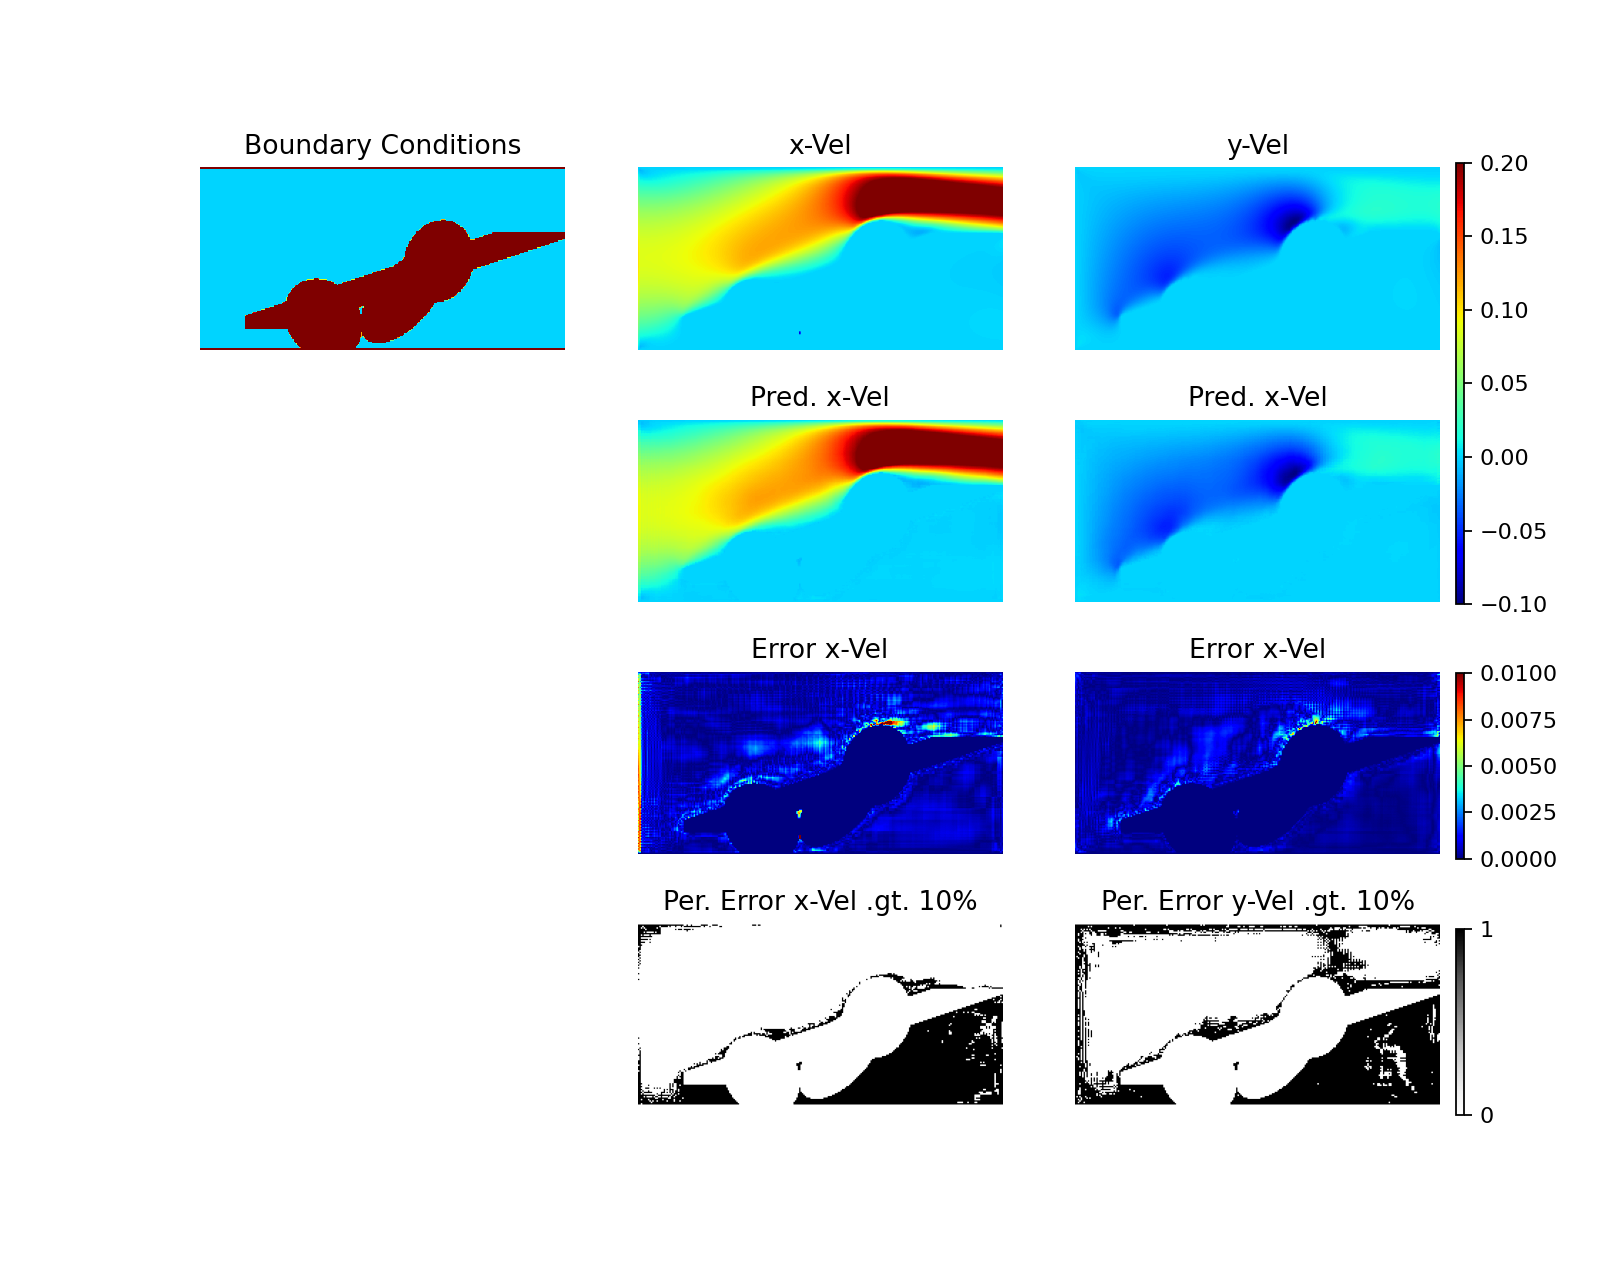
\includegraphics[width=1.0\linewidth, trim = 11.5cm 3cm 3cm 2.1cm, clip]{../../../plots/plots/test_data/montage_test_pred_0.1_81.png}%%
    \end{minipage}%
    \hspace{0.1cm}
    \begin{minipage}{0.1\textwidth}%
        \vspace{1.75cm}
        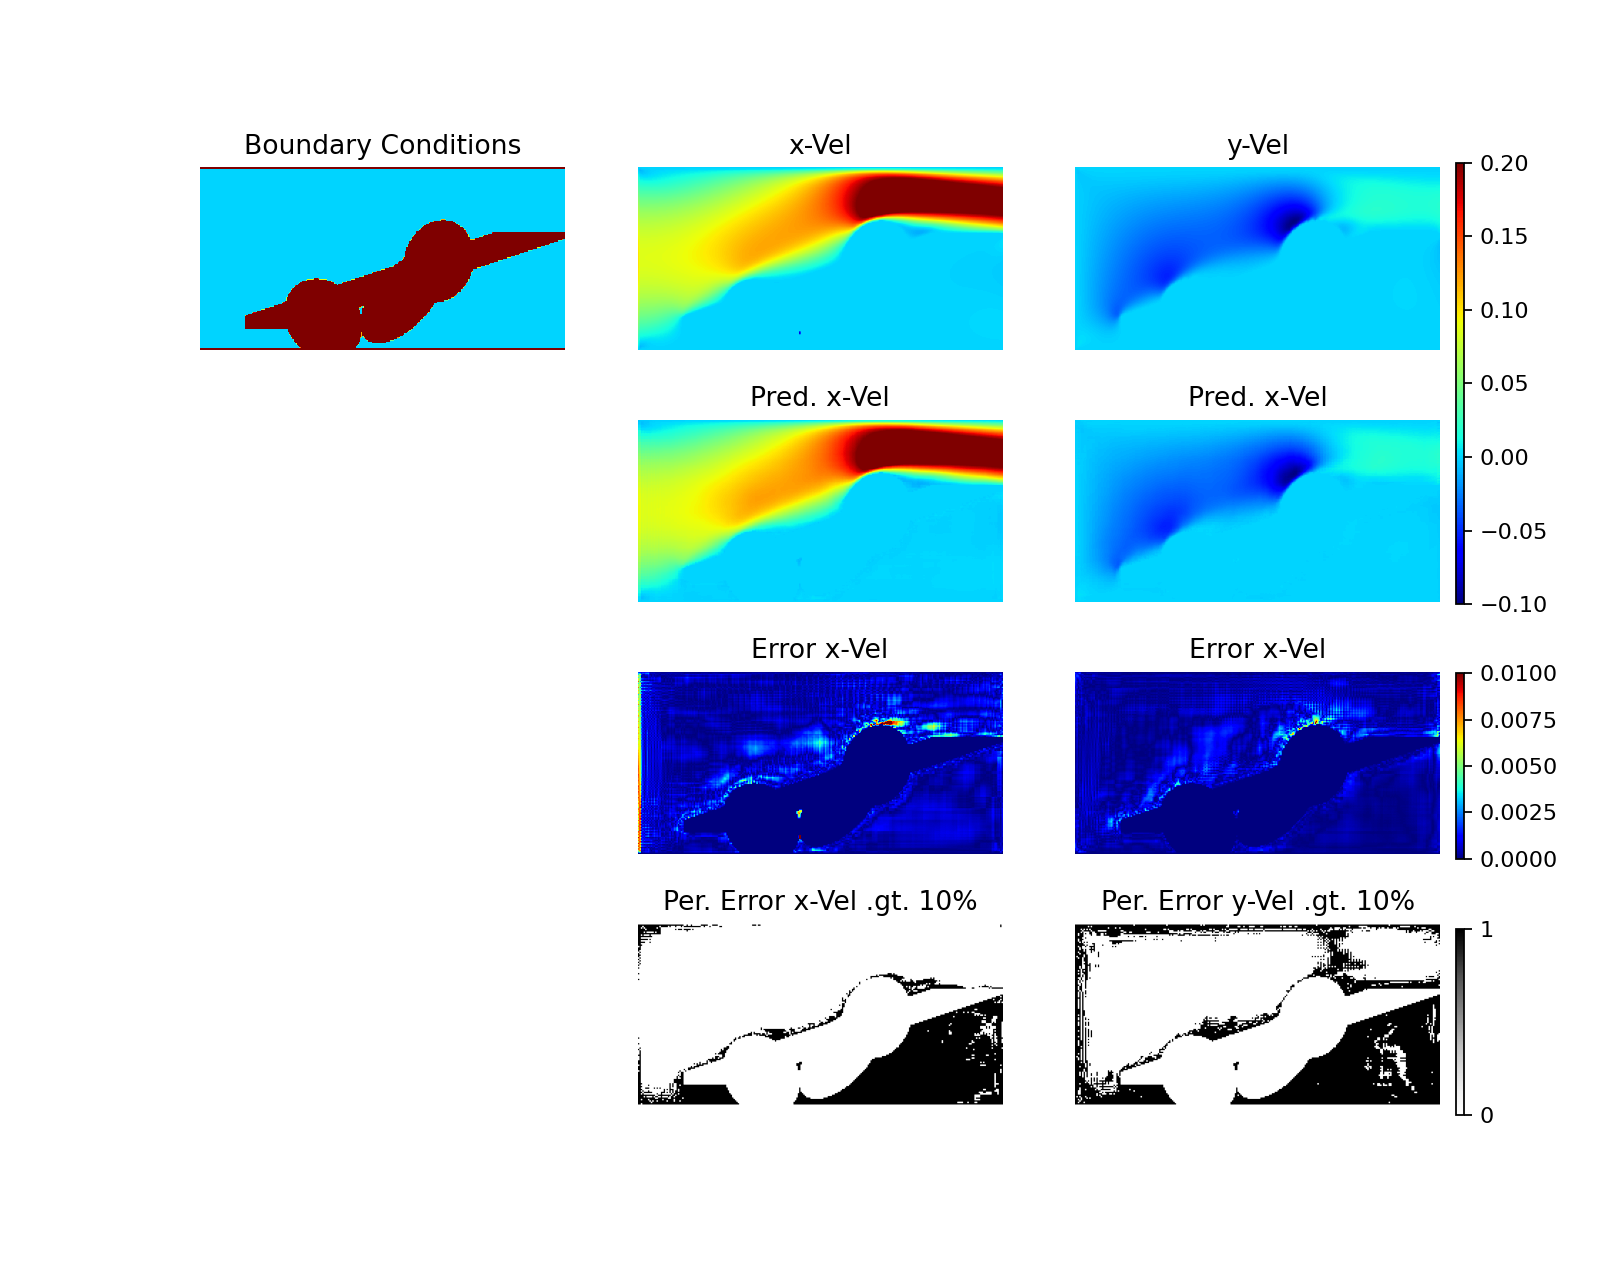
\includegraphics[width=0.49\linewidth, trim = 27.6cm 3cm 1cm 2.1cm, clip]{../../../plots/plots/test_data/montage_test_pred_0.1_81.png}%%
    \end{minipage}%
\end{figure}
\end{frame}


\begin{frame}
\frametitle{Test Data \Sadey[1.5]}
\vspace{-0.40cm}
\begin{figure}[!htb]%
    \hspace{-0.55cm}
    \begin{minipage}{0.41\textwidth}%
       \center{
       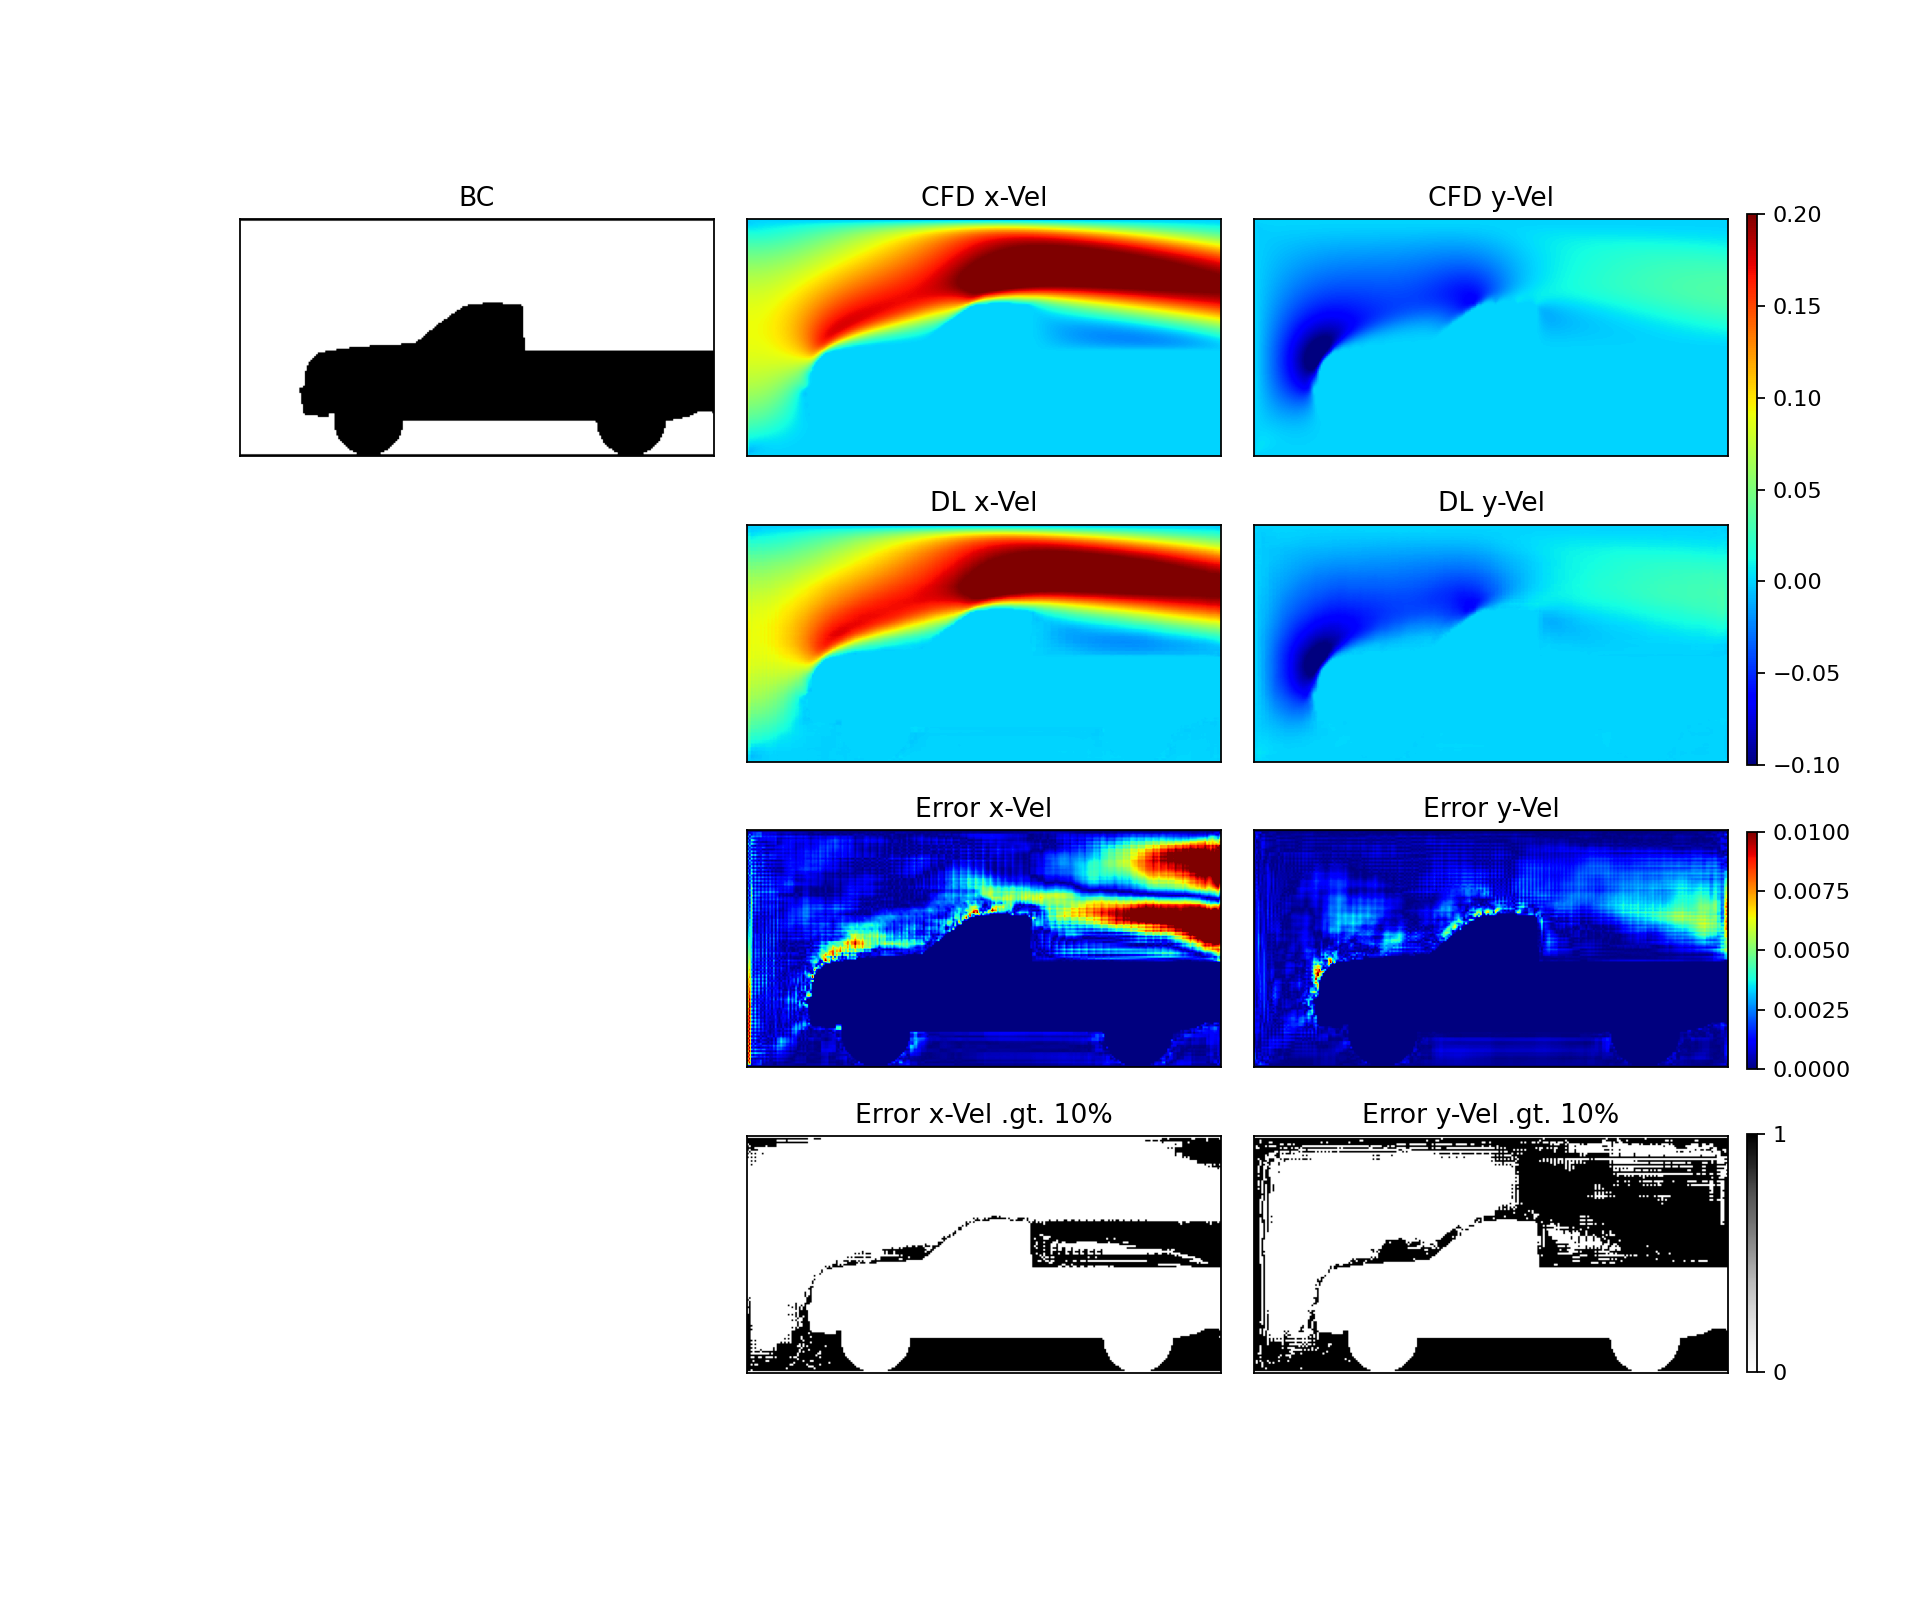
\includegraphics[width=0.5\linewidth, trim = 3.65cm 17.94cm 19.08cm 2.1cm, clip]{../../../plots/plots/test_data/montage_test_pred_0.1_26.png}%%%
       }
       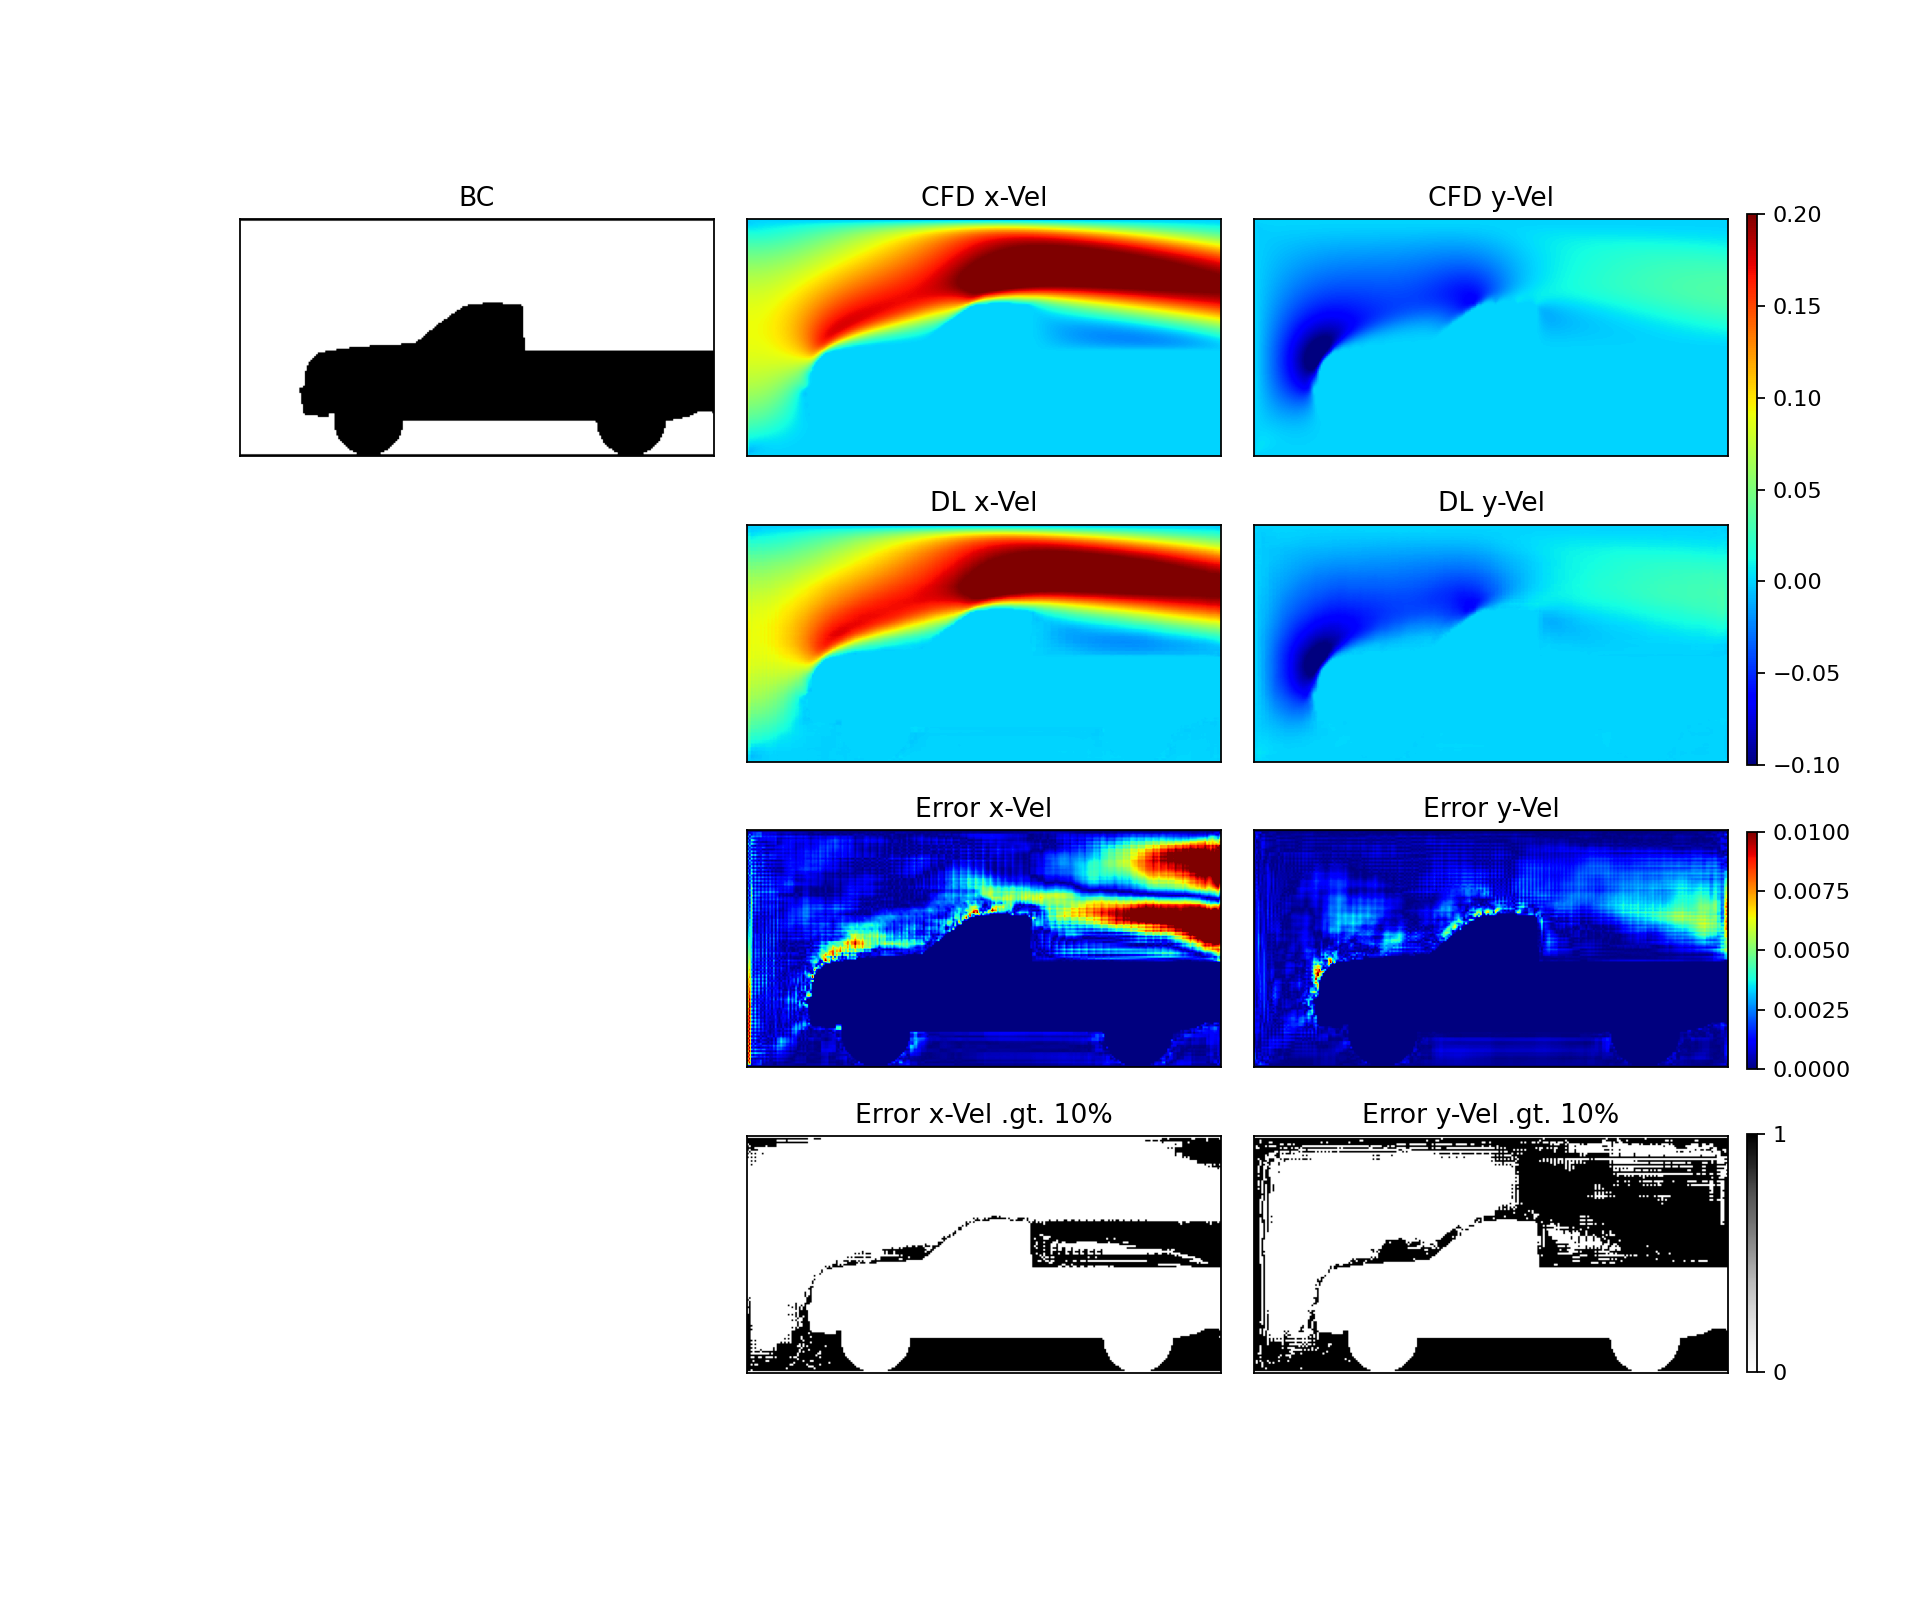
\includegraphics[width=1.0\linewidth, trim = 11.5cm 3cm 3cm 2.1cm, clip]{../../../plots/plots/test_data/montage_test_pred_0.1_26.png}%%%
    \end{minipage}%
    %
    \hspace{0.25cm}
    \begin{minipage}{0.41\textwidth}%
        \center{
        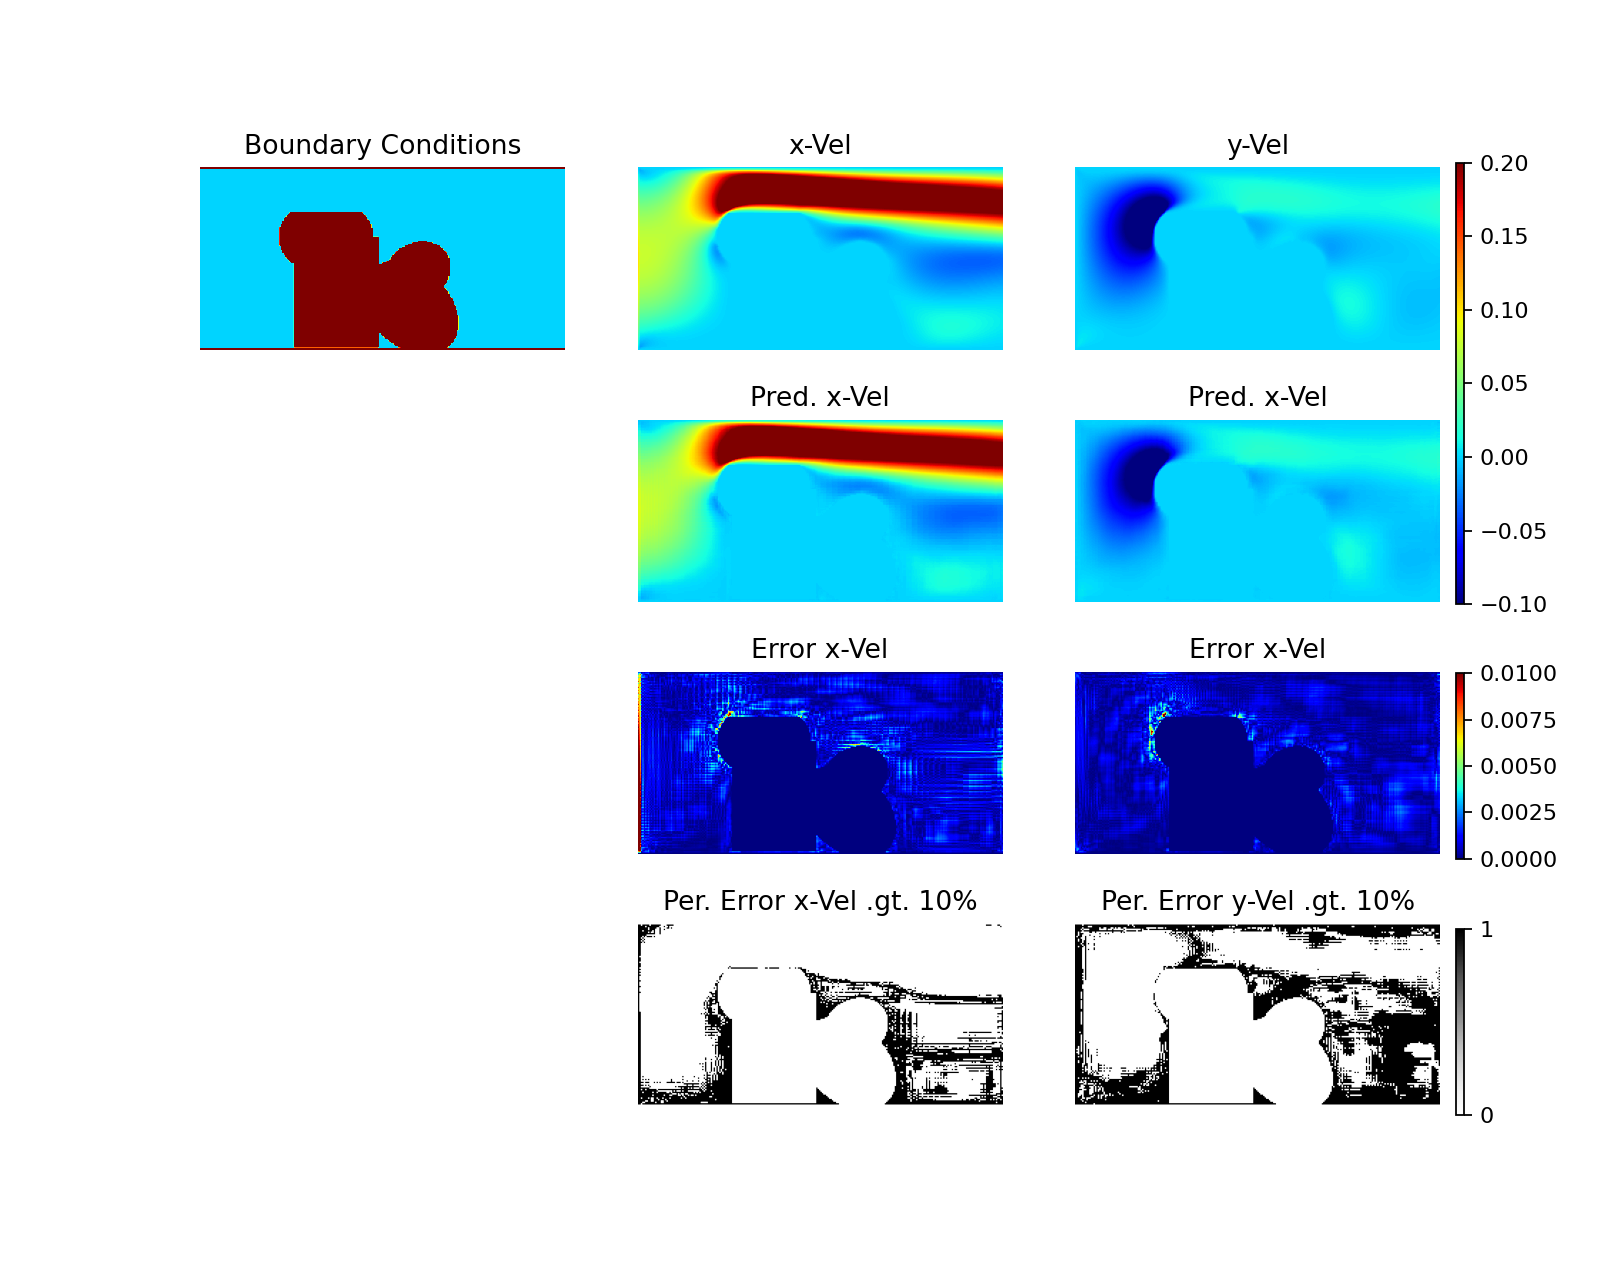
\includegraphics[width=0.5\linewidth, trim = 3.65cm 17.94cm 19.08cm 2.1cm, clip]{../../../plots/plots/test_data/montage_test_pred_0.1_50.png}%%
        }
        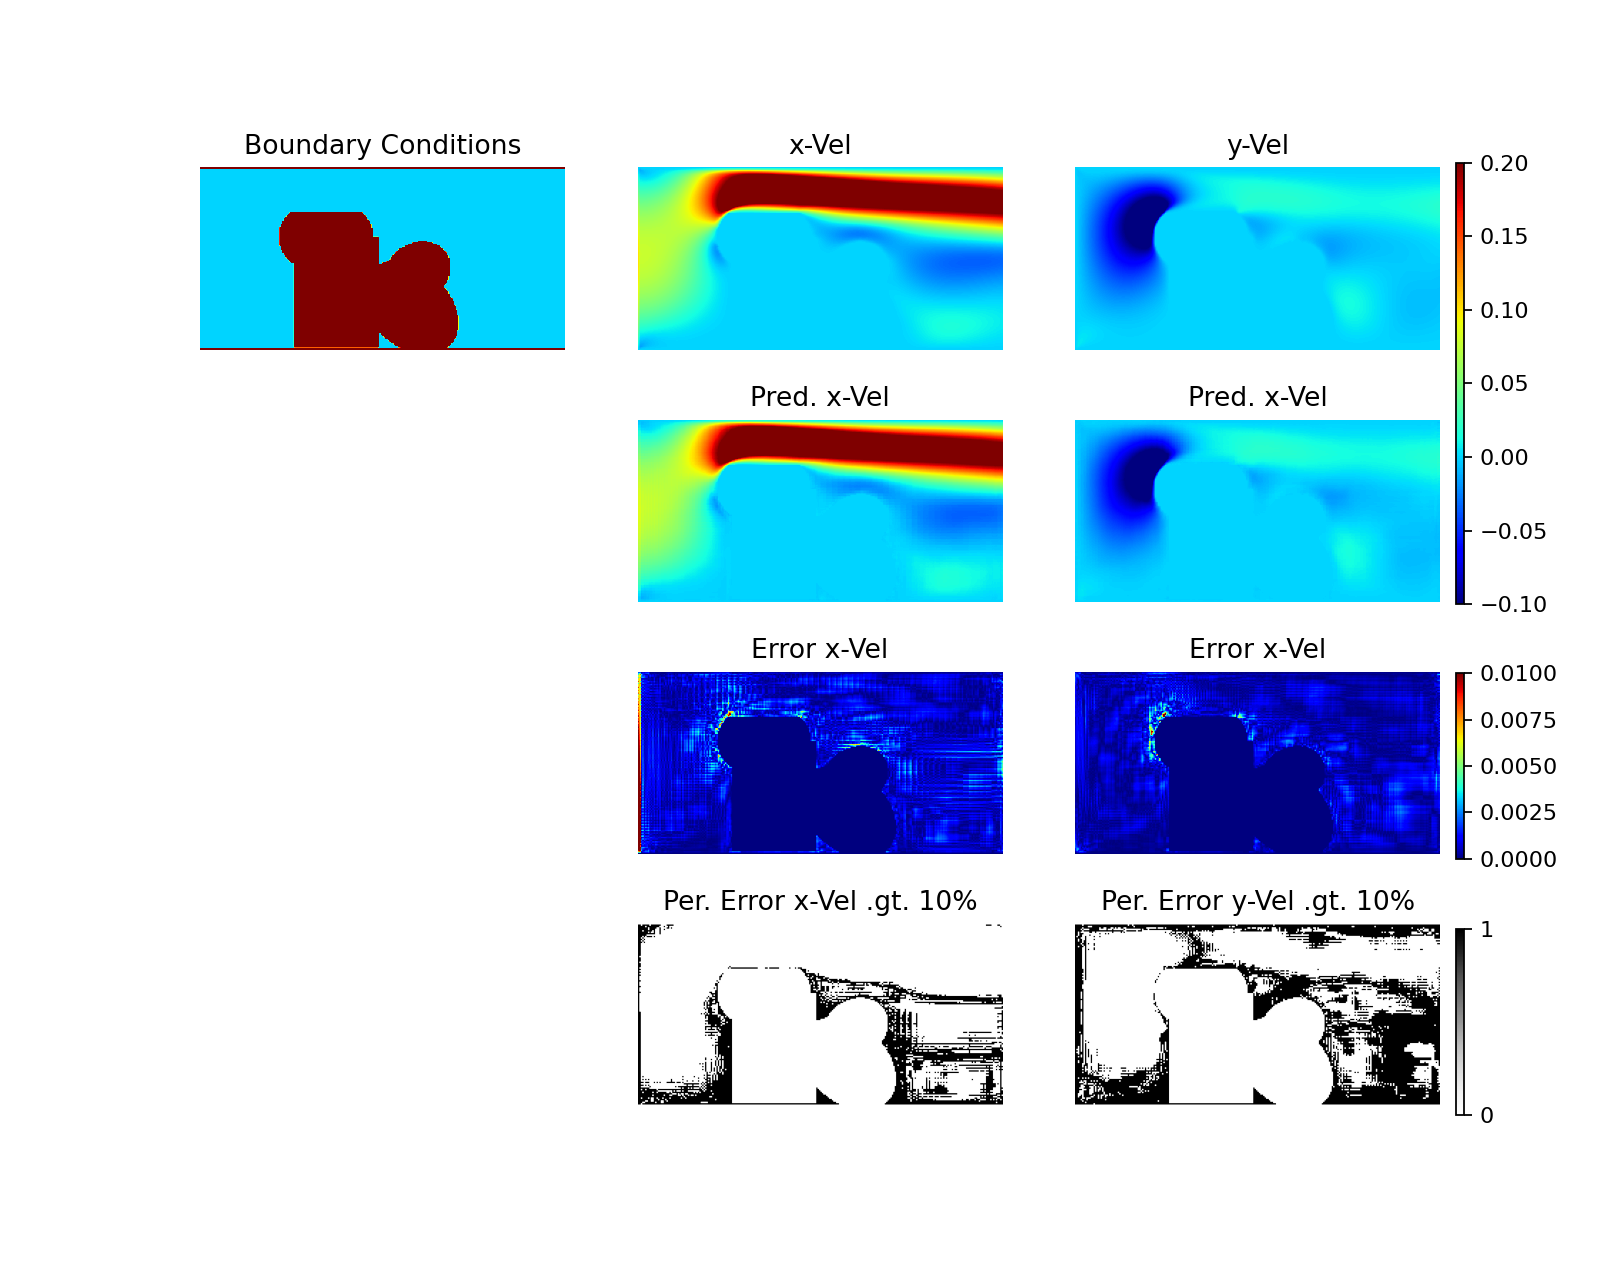
\includegraphics[width=1.0\linewidth, trim = 11.5cm 3cm 3cm 2.1cm, clip]{../../../plots/plots/test_data/montage_test_pred_0.1_50.png}%%
    \end{minipage}%
    \hspace{0.1cm}
    \begin{minipage}{0.1\textwidth}%
        \vspace{1.75cm}
        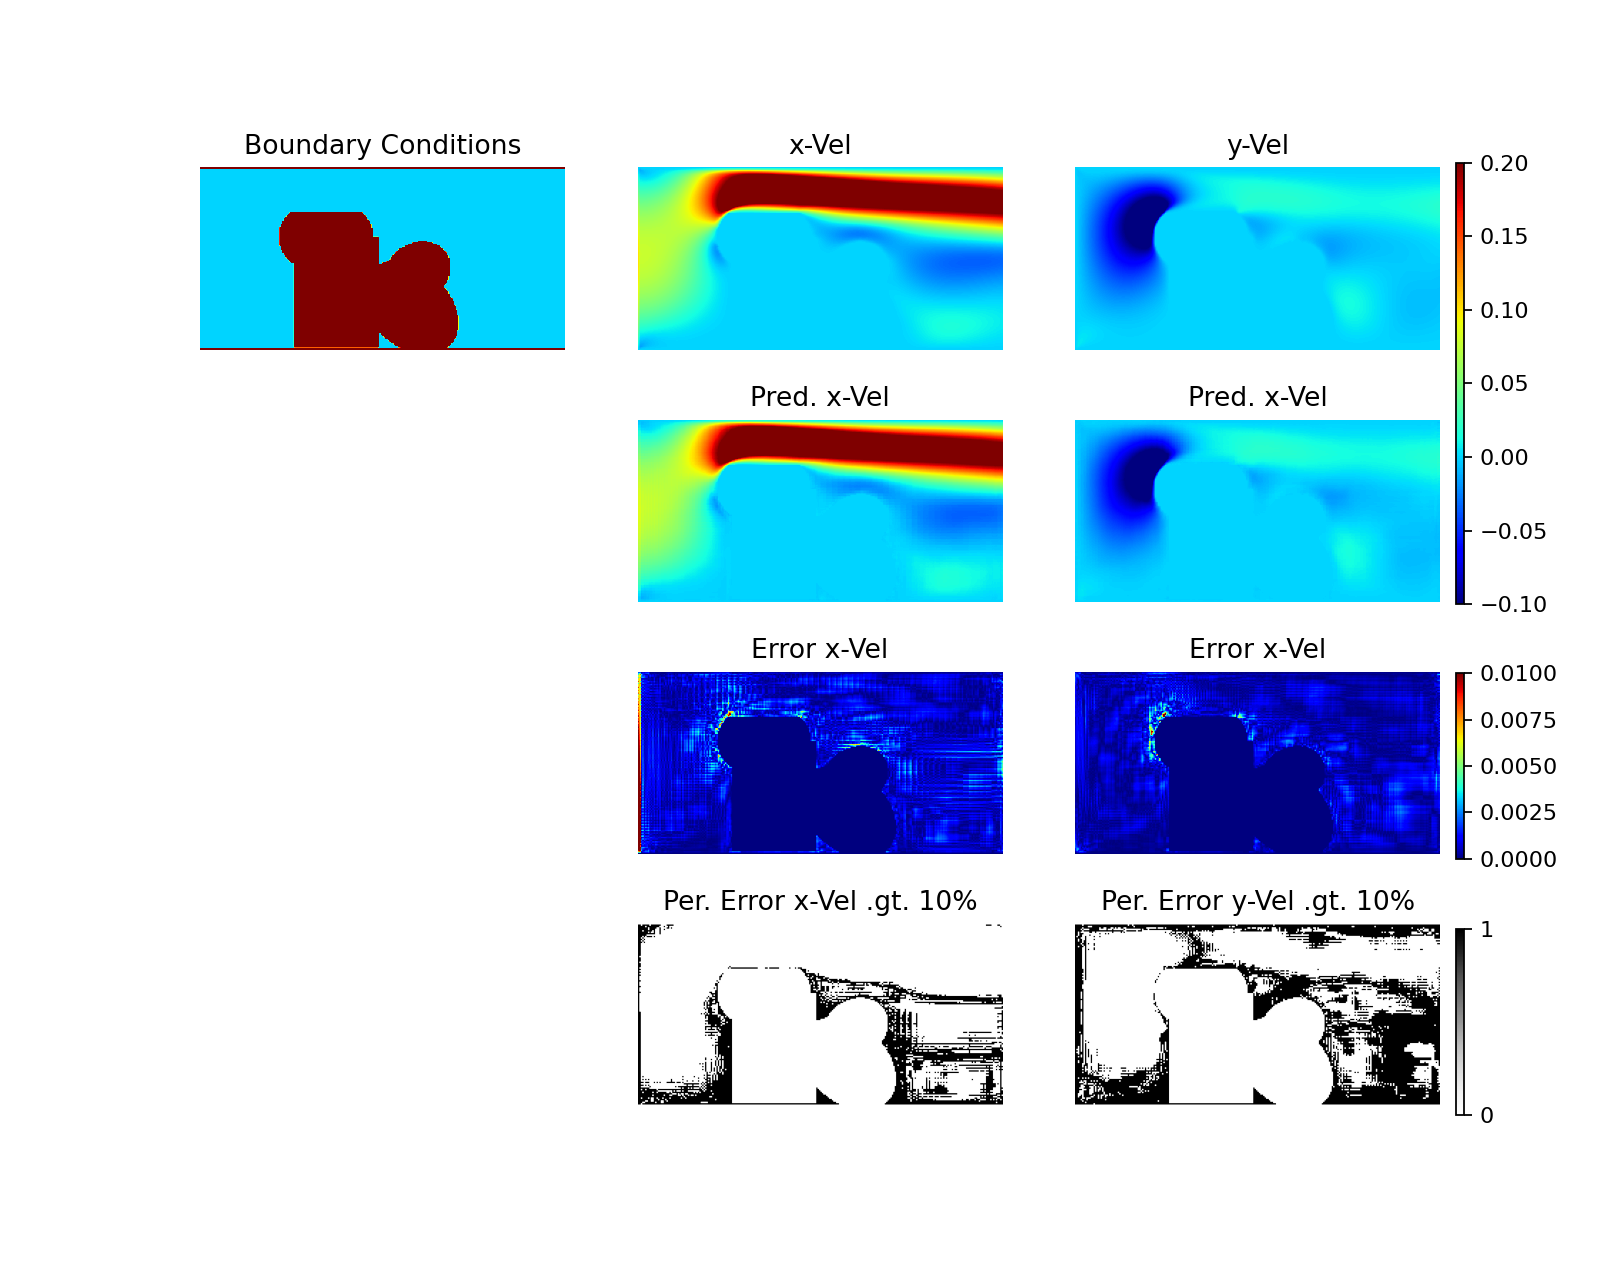
\includegraphics[width=0.49\linewidth, trim = 27.6cm 3cm 1cm 2.1cm, clip]{../../../plots/plots/test_data/montage_test_pred_0.1_50.png}%%
    \end{minipage}%
\end{figure}
\end{frame}


\begin{frame}
\frametitle{Test Data}
\begin{figure}[!htb]%
\caption{This slide contains a movie}
\end{figure}
\end{frame}


\begin{frame}
\frametitle{Train vs. Validation Data}
\begin{itemize}
\item Train/Test Data: random geometrical shapes
\item Validation Data: cars designs
\end{itemize}
\vspace{1cm}
\centering
\Huge{iid?}
\end{frame}

\begin{frame}
\frametitle{Validation Data: cars designs}
\begin{figure}[h]
%
\includegraphics[width=8cm, trim = 2cm 2cm 1cm 2cm, clip]{img/shapes.png}
%\caption{Geometry: shape variations generated randomly}
\vspace{0.4cm}
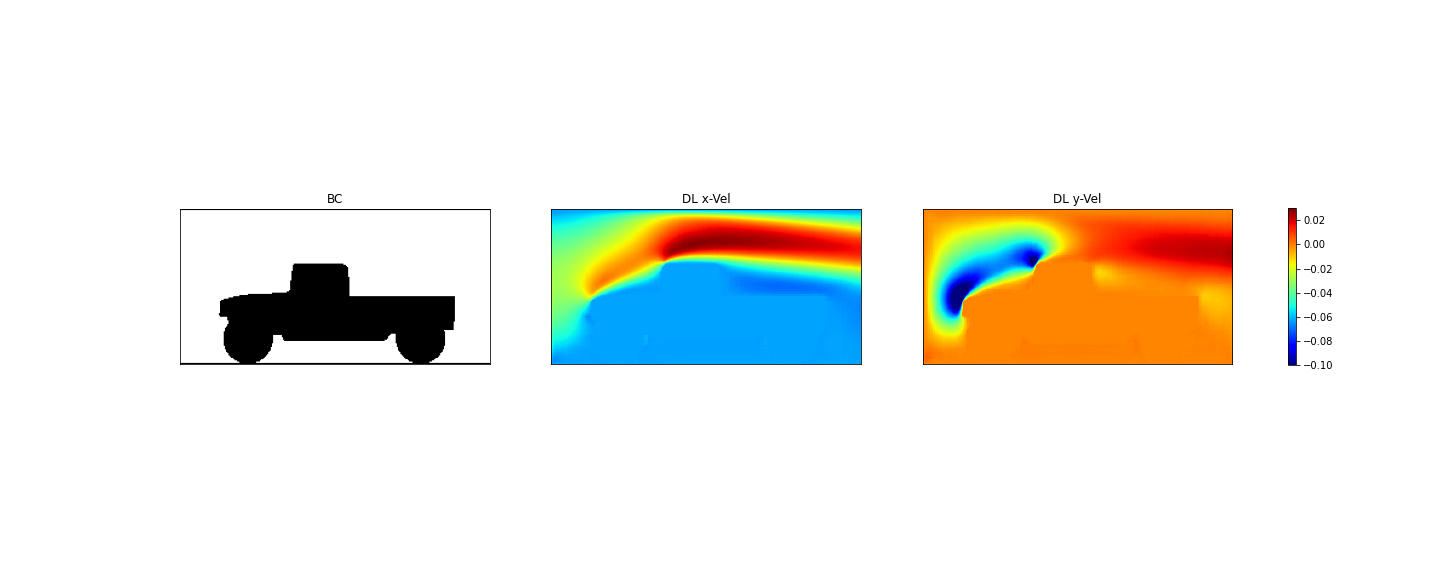
\includegraphics[height=0.16\linewidth, trim = 5.80cm 7.35cm 33.4cm 7.2cm, clip]{../../../plots/plots/cars/comparison/montage_car_DL_01.png}%      
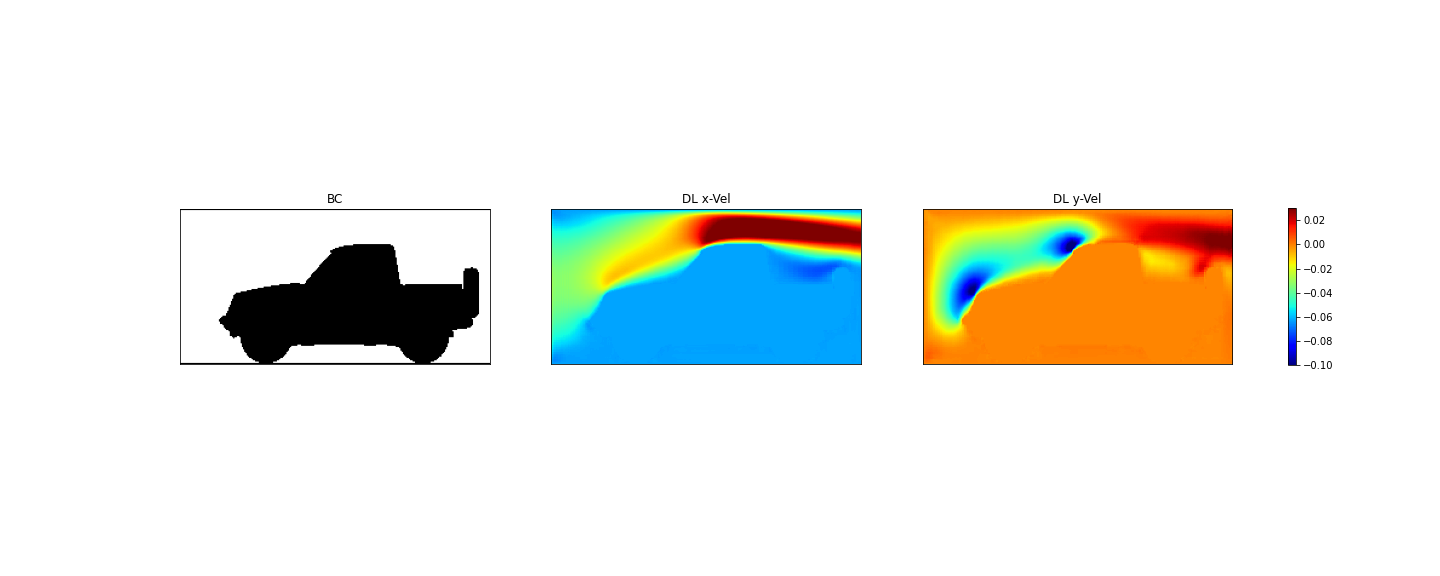
\includegraphics[height=0.16\linewidth, trim = 5.80cm 7.35cm 33.4cm 7.2cm, clip]{../../../plots/plots/cars/comparison/montage_car_DL_27.png}%
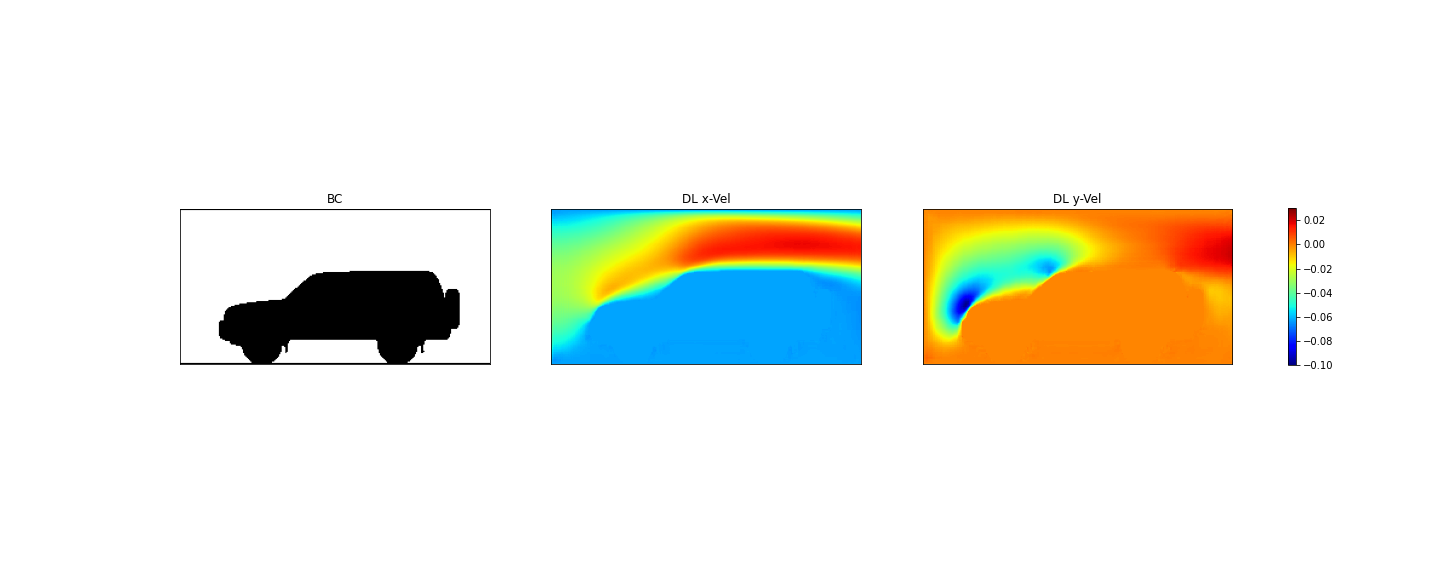
\includegraphics[height=0.16\linewidth, trim = 5.80cm 7.35cm 33.4cm 7.2cm, clip]{../../../plots/plots/cars/comparison/montage_car_DL_00.png}%

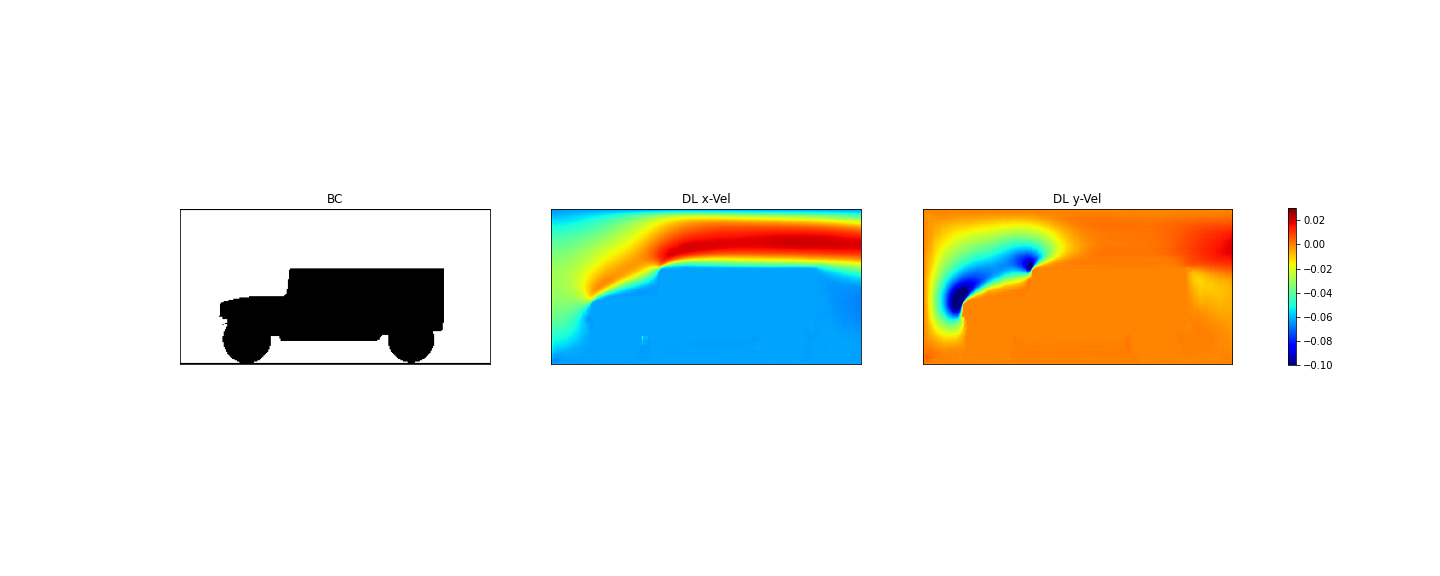
\includegraphics[height=0.16\linewidth, trim = 5.80cm 7.35cm 33.4cm 7.2cm, clip]{../../../plots/plots/cars/comparison/montage_car_DL_02.png}%      
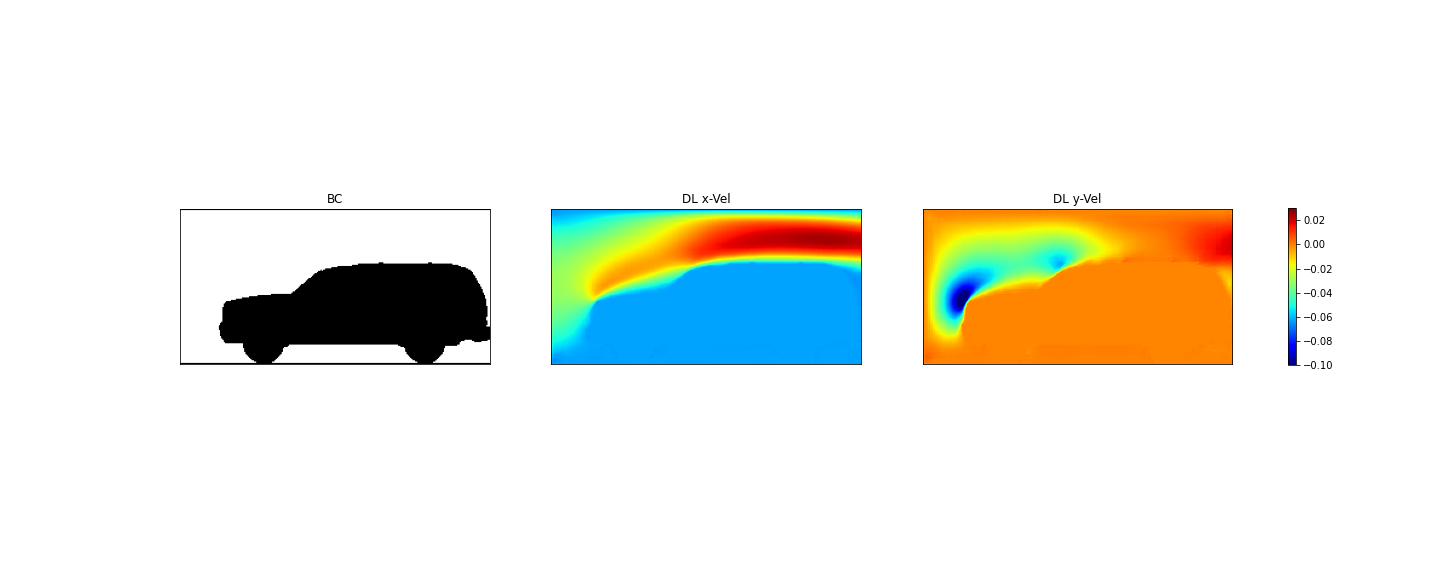
\includegraphics[height=0.16\linewidth, trim = 5.80cm 7.35cm 33.4cm 7.2cm, clip]{../../../plots/plots/cars/comparison/montage_car_DL_03.png}%
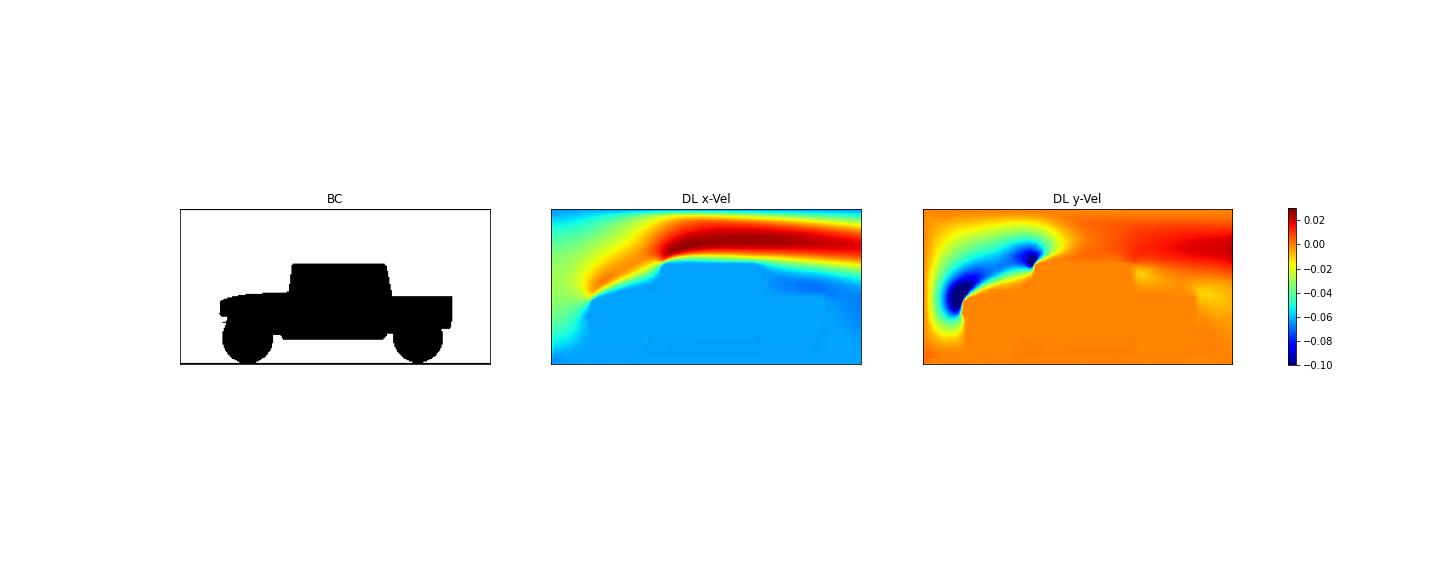
\includegraphics[height=0.16\linewidth, trim = 5.80cm 7.35cm 33.4cm 7.2cm, clip]{../../../plots/plots/cars/comparison/montage_car_DL_04.png}%

\includegraphics[height=0.16\linewidth, trim = 5.80cm 7.35cm 33.4cm 7.2cm, clip]{../../../plots/plots/cars/comparison/montage_car_DL_05.png}%      
\includegraphics[height=0.16\linewidth, trim = 5.80cm 7.35cm 33.4cm 7.2cm, clip]{../../../plots/plots/cars/comparison/montage_car_DL_06.png}%
\includegraphics[height=0.16\linewidth, trim = 5.80cm 7.35cm 33.4cm 7.2cm, clip]{../../../plots/plots/cars/comparison/montage_car_DL_07.png}%

\includegraphics[height=0.16\linewidth, trim = 5.80cm 7.35cm 33.4cm 7.2cm, clip]{../../../plots/plots/cars/comparison/montage_car_DL_08.png}%      
\includegraphics[height=0.16\linewidth, trim = 5.80cm 7.35cm 33.4cm 7.2cm, clip]{../../../plots/plots/cars/comparison/montage_car_DL_09.png}%
\includegraphics[height=0.16\linewidth, trim = 5.80cm 7.35cm 33.4cm 7.2cm, clip]{../../../plots/plots/cars/comparison/montage_car_DL_10.png}%
\end{figure}
\end{frame}

\begin{frame}
\frametitle{Validation Data}
\begin{figure}[!htb]%
\vspace{-0.20cm}
\includegraphics[height=0.20\linewidth, trim = 5.80cm 5.25cm 1.3cm 6.50cm, clip]{../../../plots/plots/cars/comparison/montage_car_DL_01.png}%
        
\includegraphics[height=0.20\linewidth, trim = 5.80cm 5.25cm 1.3cm 6.50cm, clip]{../../../plots/plots/cars/comparison/montage_car_DL_27.png}%

\includegraphics[height=0.20\linewidth, trim = 5.80cm 5.25cm 1.3cm 6.50cm, clip]{../../../plots/plots/cars/comparison/montage_car_DL_00.png}%
\vspace{-0.35cm}
\caption{BCs \& DL predictions}
\end{figure}
\end{frame}


\begin{frame}
\frametitle{Validation Data}
\begin{figure}[!htb]%
\includegraphics[height=0.28\linewidth, trim = 5.80cm 4.25cm 1.3cm 4.50cm, clip]{../../../plots/plots/cars/comparison/montage_car_DL_04.png}%
        
\includegraphics[height=0.28\linewidth, trim = 5.80cm 4.25cm 1.3cm 4.50cm, clip]{../../../plots/plots/cars/comparison/montage_car_CFD_04.png}
\caption{DL vs. CFD}
\end{figure}
\end{frame}


\begin{frame}
\frametitle{Validation Data \Smiley[1.5]}
\vspace{-0.40cm}
\begin{figure}[!htb]%
    \hspace{-0.55cm}
    \begin{minipage}{0.41\textwidth}%
       \center{
       \includegraphics[width=0.5\linewidth, trim = 3.65cm 17.94cm 19.08cm 2.1cm, clip]{../../../plots/plots/cars/errors/montage_test_pred_0.1_08.png}%%%
       }
       \includegraphics[width=1.0\linewidth, trim = 11.5cm 3cm 3cm 2.1cm, clip]{../../../plots/plots/cars/errors/montage_test_pred_0.1_08.png}%%%
    \end{minipage}%
    %
    \hspace{0.25cm}
    \begin{minipage}{0.41\textwidth}%
        \center{
        \includegraphics[width=0.5\linewidth, trim = 3.65cm 17.94cm 19.08cm 2.1cm, clip]{../../../plots/plots/cars/errors/montage_test_pred_0.1_10.png}%%
        }
        \includegraphics[width=1.0\linewidth, trim = 11.5cm 3cm 3cm 2.1cm, clip]{../../../plots/plots/cars/errors/montage_test_pred_0.1_10.png}%%
    \end{minipage}%
    \hspace{0.1cm}
    \begin{minipage}{0.1\textwidth}%
        \vspace{1.75cm}
        \includegraphics[width=0.49\linewidth, trim = 27.6cm 3cm 1cm 2.1cm, clip]{../../../plots/plots/cars/errors/montage_test_pred_0.1_10.png}%%
    \end{minipage}%
\end{figure}
\end{frame}


\begin{frame}
\frametitle{Validation Data \Sadey[1.5]}
\vspace{-0.40cm}
\begin{figure}[!htb]%
    \hspace{-0.55cm}
    \begin{minipage}{0.41\textwidth}%
       \center{
       \includegraphics[width=0.5\linewidth, trim = 3.65cm 17.94cm 19.08cm 2.1cm, clip]{../../../plots/plots/cars/errors/montage_test_pred_0.1_11.png}%%%
       }
       \includegraphics[width=1.0\linewidth, trim = 11.5cm 3cm 3cm 2.1cm, clip]{../../../plots/plots/cars/errors/montage_test_pred_0.1_11.png}%%%
    \end{minipage}%
    %
    \hspace{0.25cm}
    \begin{minipage}{0.41\textwidth}%
        \center{
        \includegraphics[width=0.5\linewidth, trim = 3.65cm 17.94cm 19.08cm 2.1cm, clip]{../../../plots/plots/cars/errors/montage_test_pred_0.1_07.png}%%
        }
        \includegraphics[width=1.0\linewidth, trim = 11.5cm 3cm 3cm 2.1cm, clip]{../../../plots/plots/cars/errors/montage_test_pred_0.1_07.png}%%
    \end{minipage}%
    \hspace{0.1cm}
    \begin{minipage}{0.1\textwidth}%
        \vspace{1.75cm}
        \includegraphics[width=0.49\linewidth, trim = 27.6cm 3cm 1cm 2.1cm, clip]{../../../plots/plots/cars/errors/montage_test_pred_0.1_07.png}%%
    \end{minipage}%
\end{figure}
\end{frame}




\begin{frame}
\frametitle{Validation Data}
\begin{figure}[!htb]%
\caption{This slide contains a movie}
\end{figure}
\end{frame} 

\begin{frame}
\frametitle{Training Loss}
\begin{figure}[h]
\hspace{-1cm}
\includegraphics[width=12cm,trim = 0cm 0cm 13cm 0cm, clip]{../../../plots/all_history.png}
\end{figure}
\end{frame}
%------------------------------------------------

\section{Further Work} % A subsection can be created just before a set of slides with a common theme to further break down your presentation into chunks

\begin{frame}
\frametitle{Further Work}
\begin{itemize}
\item Better Loss/Metrics Function
\item More Training Data
\item Increase Training Time
\item Improve architecture
\end{itemize}
\end{frame}


%\begin{frame}
%\printbibliography
%\Huge{\centerline{The End}}
%\end{frame}
\begin{frame}[t,allowframebreaks]
\frametitle{References}
\begin{refsection}
%\nocite{*}
\printbibliography[keyword=secondary, title={List of Publications}]
\end{refsection}
%\cite{wombat2016}
%\bibliographystyle{amsalpha}
\printbibliography
\end{frame}

%----------------------------------------------------------------------------------------

\end{document} 

\subsection{Subsection Example} % A subsection can be created just before a set of slides with a common theme to further break down your presentation into chunks

\begin{frame}
\frametitle{Paragraphs of Text}
Sed iaculis dapibus gravida. Morbi sed tortor erat, nec interdum arcu. Sed id lorem lectus. Quisque viverra augue id sem ornare non aliquam nibh tristique. Aenean in ligula nisl. Nulla sed tellus ipsum. Donec vestibulum ligula non lorem vulputate fermentum accumsan neque mollis.\\~\\

Sed diam enim, sagittis nec condimentum sit amet, ullamcorper sit amet libero. Aliquam vel dui orci, a porta odio. Nullam id suscipit ipsum. Aenean lobortis commodo sem, ut commodo leo gravida vitae. Pellentesque vehicula ante iaculis arcu pretium rutrum eget sit amet purus. Integer ornare nulla quis neque ultrices lobortis. Vestibulum ultrices tincidunt libero, quis commodo erat ullamcorper id.
\end{frame}

%------------------------------------------------

\begin{frame}
\frametitle{Bullet Points}
\begin{itemize}
\item Lorem ipsum dolor sit amet, consectetur adipiscing elit
\item Aliquam blandit faucibus nisi, sit amet dapibus enim tempus eu
\item Nulla commodo, erat quis gravida posuere, elit lacus lobortis est, quis porttitor odio mauris at libero
\item Nam cursus est eget velit posuere pellentesque
\item Vestibulum faucibus velit a augue condimentum quis convallis nulla gravida
\end{itemize}
\end{frame}

%------------------------------------------------

\begin{frame}
\frametitle{Blocks of Highlighted Text}
\begin{block}{Block 1}
Lorem ipsum dolor sit amet, consectetur adipiscing elit. Integer lectus nisl, ultricies in feugiat rutrum, porttitor sit amet augue. Aliquam ut tortor mauris. Sed volutpat ante purus, quis accumsan dolor.
\end{block}

\begin{block}{Block 2}
Pellentesque sed tellus purus. Class aptent taciti sociosqu ad litora torquent per conubia nostra, per inceptos himenaeos. Vestibulum quis magna at risus dictum tempor eu vitae velit.
\end{block}

\begin{block}{Block 3}
Suspendisse tincidunt sagittis gravida. Curabitur condimentum, enim sed venenatis rutrum, ipsum neque consectetur orci, sed blandit justo nisi ac lacus.
\end{block}
\end{frame}

%------------------------------------------------

\begin{frame}
\frametitle{Multiple Columns}
\begin{columns}[c] % The "c" option specifies centered vertical alignment while the "t" option is used for top vertical alignment

\column{.45\textwidth} % Left column and width
\textbf{Heading}
\begin{enumerate}
\item Statement
\item Explanation
\item Example
\end{enumerate}

\column{.5\textwidth} % Right column and width
Lorem ipsum dolor sit amet, consectetur adipiscing elit. Integer lectus nisl, ultricies in feugiat rutrum, porttitor sit amet augue. Aliquam ut tortor mauris. Sed volutpat ante purus, quis accumsan dolor.

\end{columns}
\end{frame}

%------------------------------------------------
\section{Second Section}
%------------------------------------------------

\begin{frame}
\frametitle{Table}
\begin{table}
\begin{tabular}{l l l}
\toprule
\textbf{Treatments} & \textbf{Response 1} & \textbf{Response 2}\\
\midrule
Treatment 1 & 0.0003262 & 0.562 \\
Treatment 2 & 0.0015681 & 0.910 \\
Treatment 3 & 0.0009271 & 0.296 \\
\bottomrule
\end{tabular}
\caption{Table caption}
\end{table}
\end{frame}

%------------------------------------------------

\begin{frame}
\frametitle{Theorem}
\begin{theorem}[Mass--energy equivalence]
$E = mc^2$
\end{theorem}
\end{frame}

%------------------------------------------------

\begin{frame}[fragile] % Need to use the fragile option when verbatim is used in the slide
\frametitle{Verbatim}
\begin{example}[Theorem Slide Code]
\begin{verbatim}
\begin{frame}
\frametitle{Theorem}
\begin{theorem}[Mass--energy equivalence]
$E = mc^2$
\end{theorem}
\end{frame}\end{verbatim}
\end{example}
\end{frame}

%------------------------------------------------

\begin{frame}
\frametitle{Figure}
Uncomment the code on this slide to include your own image from the same directory as the template .TeX file.
%\begin{figure}
%\includegraphics[width=0.8\linewidth]{test}
%\end{figure}
\end{frame}

%------------------------------------------------

\begin{frame}[fragile] % Need to use the fragile option when verbatim is used in the slide
\frametitle{Citation}
An example of the \verb|\cite| command to cite within the presentation:\\~

This statement requires citation \cite{p1}.
\end{frame}

%------------------------------------------------

%\begin{frame}
%\frametitle{References}
%\footnotesize{
%\begin{thebibliography}{99} % Beamer does not support BibTeX so references must be inserted manually as below
%\bibitem[Smith, 2012]{p1} John Smith (2012)
%\newblock Title of the publication
%\newblock \emph{Journal Name} 12(3), 45 -- 678.
%\end{thebibliography}
%}
%\end{frame}

